%\nonstopmode
%\nonstopmode
\documentclass[letterpaper,oneside, openright]{scrbook}
\usepackage[left=32mm,right=32mm,top=32mm,bottom=32mm, headsep=10mm]{geometry}
\usepackage{color}
\usepackage{transparent}
\usepackage[round,authoryear]{natbib}

\usepackage[xindy,nonumberlist,nopostdot]{glossaries}

\usepackage[utf8]{inputenc}

\usepackage{tikz,titlesec}
\usetikzlibrary{calc}
\usepackage{setspace}
\usepackage{fancyhdr}                    
\usepackage{colortbl}
\usepackage[T1]{fontenc}
\usepackage{lmodern}

\usepackage{siunitx}
\usepackage{mhchem}

\usepackage{lipsum}
\usepackage{graphicx}
\graphicspath{{../figs/}{../figs/lit-review/}{../figs/memory-trace/}{../figs/miniscope/}}
\DeclareGraphicsExtensions{.jpg,.png,.pdf,.svg}

\usepackage{caption}
\captionsetup{labelfont=bf,format=plain,labelsep=space}
\usepackage{subcaption}
\captionsetup{subrefformat=parens}

\usepackage{verbatim} %for multiline comments
\usepackage{placeins} %for confining figures to sections

\titlespacing*{\chapter}{0pt}{4ex}{1ex}%pbk

\titleformat{\chapter}[display]
            {\Huge\filleft\scshape}
            {\normalfont\bf\fontfamily{put}\fontseries{b}\fontsize{95pt}{0pt}\selectfont\thechapter}
            {0pt}
            {}[\titlerule\vspace{2ex}\filright\vspace{2ex}]
%
\titlespacing*{\part}{-10pt}{120pt}{-80pt}%pbk

\titleformat{\part}[frame]
            {\Huge\filcenter\scshape}
            {\normalfont\bf\fontsize{85pt}{0pt}\selectfont \raisebox{1.7cm}{ Part\fontfamily{put}\fontseries{b}\fontsize{105pt}{0pt}\selectfont \hspace{.2em}\thepart} }
            {30pt}
            {}[\filright]
\addtokomafont{section}{\bfseries}
\addtokomafont{subsection}{\bfseries}
\addtokomafont{subsubsection}{\bfseries}
 \titleformat{\section}[hang]%
     {\usekomafont{section}}%
     {\thesection\hspace{.5em}}%
     {.0em}%
     {\filright}%


 \titleformat{\subsection}[hang]%
     {\usekomafont{subsection}}%
     {\thesubsection\hspace{.5em}}%
     {.0em}%
     {\filright}%
 \titleformat{\subsubsection}[hang]%
     {\usekomafont{subsubsection}}%
     {\thesubsubsection\hspace{.5em}}%
     {.0em}%
     {\filright}%


\addtokomafont{chapterentry}{\rmfamily\large}


     %%% Fancy Header %%%%%%%%%%%%%%%%%%%%%%%%%%%%%%%%%%%%%%%%%%%%%%%%%%%%%%%%%%%%%%%%%%
     % Fancy Header Style Options

\fancypagestyle{body}{                       % Sets fancy header and footer
    \fancyfoot{}                            % Delete current footer settings

    %\renewcommand{\chaptermark}[1]{         % Lower Case Chapter marker style
    %  \markboth{\chaptername\ \thechapter.\ #1}}{}} %

    %\renewcommand{\sectionmark}[1]{         % Lower case Section marker style
    %  \markright{\thesection.\ #1}}         %

    \fancyhead[LE,RO]{\oldstylenums{\thepage}}    % Page number (boldface) in left on even
% pages and right on odd pages
    \renewcommand{\chaptermark}[1]{\markboth{\MakeUppercase{\thechapter.\ ##1}}{}}
    \fancyhead[RE]{\bfseries\scshape\nouppercase{\leftmark}}      % Chapter in the right on even pages
    \fancyhead[LO]{\bfseries\scshape\nouppercase{\rightmark}}     % Section in the left on odd pages

    \let\headruleORIG\headrule
    \renewcommand{\headrule}{\color{black} \headruleORIG}
    \renewcommand{\headrulewidth}{.5pt}
    \arrayrulecolor{black}
}

\fancypagestyle{plain}{
    \fancyhead{}
  \fancyfoot{}%[CE,CO]{\oldstylenums{\thepage}}
  \renewcommand{\headrulewidth}{0pt}
  \renewcommand{\footrulewidth}{0.0pt}
}

\fancypagestyle{preliminary}{
    \fancyhead{}
    \fancyfoot[CE,CO]{\oldstylenums{\thepage}}
    \renewcommand{\headrulewidth}{0pt}
    \renewcommand{\footrulewidth}{0pt}
}


\renewcommand{\figurename}{Figure~}

\DeclareSIUnit{\Molar}{\textsc{m}}

%confine figures to sections
\let\Oldsection\section
\renewcommand{\section}{\FloatBarrier\Oldsection}

\let\Oldsubsection\subsection
\renewcommand{\subsection}{\FloatBarrier\Oldsubsection}

\let\Oldsubsubsection\subsubsection
\renewcommand{\subsubsection}{\FloatBarrier\Oldsubsubsection}


 %% The following five commands set the respective field values so we can
 %% generate the title page and abstract page automatically.
\newcommand*{\degree}[1]%
  {\ifx\empty#1\empty\else\gdef\vdegree{#1}\fi}
\newcommand*{\department}[1]%
  {\ifx\empty#1\empty\else\gdef\vdepartment{#1}\fi}
\newcommand*{\gradyear}[1]%
  {\ifx\empty#1\empty\else\gdef\vgradyear{#1}\fi}
\renewcommand*{\author}[1]%
  {\ifx\empty#1\empty\else\gdef\vauthor{#1}\fi}
\renewcommand*{\title}[1]%
  {\ifx\empty#1\empty\else\gdef\vtitle{#1}\fi}

  %\newcommand*{\singlespacingnoskip}{\setstretch{\setspace@singespace}}

  %% Change \maketitle to follow SGS guidelines.
\renewcommand{\maketitle}%
  {\begin{titlepage}
  \large\doublespacing
      \begin{center}
          \mbox{}
          \vfill
          \textsc{\huge\vtitle}
          \vfill
      \end{center}
      \singlespacing
      \begin{center}
          by \\
          \vfill
          {\Large\vauthor}\\
          \vfill
          \vfill
          A thesis submitted in conformity with the requirements\\
          for the degree of {\vdegree}\\
          {\vdepartment}\\
          University of Toronto\\
          \vfill
          {\copyright} Copyright {\vgradyear} by {\vauthor}\\
          \vspace{.01\textheight}
          \mbox{}
      \end{center}
      \setcounter{page}{1}
  \end{titlepage}
   \setcounter{page}{2}}

\newenvironment{abstract}%
  {
      \chapter*{Abstract}
   \begin{center}
       {\Large\textbf\vtitle}\\[2ex]
       {\vauthor}\\
       {\vdegree}\\
       {\vdepartment}\\
       University of Toronto\\
       {\vgradyear}\\
   \end{center}
   \begingroup
   %% Adjust line spacing: if it was less than 2, increase it to 2;
   %% otherwise, leave it as is.
   \ifdim \baselinestretch pt < 1.6pt \doublespacing\fi}%
  {\par\endgroup\newpage}


  %% \begin{acknowledgements}...\end{acknowledgements} formats an
  %% acknowledgements section (*not* on a separate page).
\newenvironment{acknowledgements}%
  {
      \chapter*{Acknowledgements}
   \begingroup\noindent}%
  {\par\endgroup\newpage}



  %% Single-spaced quotes and quotations.
\newenvironment{longquote}%
  {\begin{quote}\singlespacingnoskip}{\end{quote}}
      \newenvironment{longquotation}%
  {\begin{quotation}\singlespacingnoskip}{\end{quotation}}

\newcommand{\us}[2]{\underset{#1}{\operatorname{#2}}}

\draft

%% *** Change this example to appropriate values. ***
\degree{Doctor of Philosophy}
\department{Institute of Medical Science}
\gradyear{2017}
\author{Chen Yan}
\title{Developing and using a head-mounted miniature microscope to investigate memory formation in mouse model of Alzheimer's Disease}

\loadglsentries{abbr}
\setacronymstyle{long-short}
\makeglossaries
\makeindex


\setcounter{tocdepth}{3}

%% Make each page fill up the entire page.
\flushbottom
\doublespacing

\usepackage{todonotes}


%%%%%%%%%%%%      MAIN  DOCUMENT      %%%%%%%%%%%%

\begin{document}
\pagenumbering{roman}
\pagestyle{preliminary}
\renewcommand*\chapterpagestyle{preliminary}

\newcommand\tglu{TAT-GluA2\textsubscript{3Y}}
\newcommand\glu{GluA2\textsubscript{3Y}}
\newcommand\tsb[1]{\textsubscript{#1}}
\newcommand\tsp[1]{\textsuperscript{#1}}
\newcommand\abeta[1][]{\gls{abeta}\textsubscript{#1}}
\newcommand\atau[1][]{\textit{tau}}

\frontmatter

\maketitle

\begin{abstract}
    \Gls{ad} is characterized by progressive memory loss. While \abeta{} is widely implicated in the pathophysiology of \gls{ad}, how an impairment of neural function on the molecular and cellular level by \abeta{} creates cognitive deficits in \gls{ad} is still unknown. To investigate the circuitry deficit in the \gls{ad}, I first developed a miniature fluorescent microscope for \textit{in vivo} calcium imaging. We have showed that the mini-microscope is able to image hundreds of neurons in hippocampal \gls{ca1} simultaneously in freely behaving mice. Moreover, we have shown that the mini-microscope is able to imaging deep brain regions such as \gls{la}, and in two different colour channels. 

We then used the mini-microscope to image in a mouse model of early \gls{ad}, TgCRND8, and hypothesized that an impairment of circuitry function underlies the cognitive deficit in these mice, and that rescuing the behavioural deficit by enhancing \gls{ltp} is able to restore the circuitry function of the \gls{ad} mice. We trained the \gls{ad} and \gls{wt} mice in contextual fear conditioning while imaging dorsal hippocampal \gls{ca1} neurons using the mini-microscope. We found while the \gls{ad} mice shows a deficit during memeory test, the memory deficit is present as a significantly shortened freezing bouts, but without a significant decrease of the number of freezing bouts. Mini-microscope recording data show that \gls{ca1} cells in the \gls{ad} mice has significant hyperexcitability and less information content about memory recall. Moreover, we have found the pattern completion process, which is important for recalling hippocampal dependent memory, is impaired in the \gls{ad} mice, represented as a lack of coordination between \gls{ca1} neuron activities. 

Moreover, we found that blocking \gls{ampa} endocytosis using \tglu{} is able to rescue both the behaviour and circuitry deficit in the \gls{ad} mice. Furthermore, we have also found that the memory deficit in the \gls{ad} mice is a deficit of memory recall, since \tglu treatment during a reminder one day ofter training is able to rescue the memory deficit, suggesting \gls{ad} mice can still retain the memory one day after training. 

In this thesis, I have shown that new development in calcium imaging is able to help study the circuitry function of the brain. In the \gls{ad} project, the results suggest that the abberation of neural circuitry function is important in producing the cognitive symptoms in \gls{ad}. Our findings also provide a link from cellular deficit in \gls{ad} to neural circuitry and finally behavioural deficit. 



\end{abstract}

\begin{acknowledgements}
    I am among the lucky few to enter graduate school under the exceptional mentorship of Dr.~Sheena Josselyn, and it's hard to overstate my gratitude for Sheena's motivation, guidance and advice over my PhD program. Sheena's unwavering encouragement and support gave me the courage to transition from molecular biology to engineering and computational neuroscience with no prior experience, and made the journey extremely fulfilling. Sheena has shown me what an iconic scientist is: knowledgeable yet humble, rigorous yet open-minded, passionate yet meticulous, and these attributes are what I will strive to achieve. I would also like to thank my program advisory committee members: Dr.~Junchul Kim, Dr.~Christopher Yip and Dr.~Fang Liu. Your suggestions and feedback during committee meetings has been very helpful, and greatly pushed the project forward. 

I would like to thank Dr.~Paul Frankland for always being helpful and supportive, and providing great new ideas for experiments and analysis. I have been tremendously privileged to work with the brilliant members of the Josselyn \slash{} Frankland lab during the PhD program. I would like to express my gratitude to Dr.~Valentina Mercaldo, who volunteered to be the unfortunate pilot user of the bug-ridden mini-microscope prototype and actually endured it --- this work would not exist if not for her unreasonable perseverance and enthusiasm. Furthermore, I would like to thank Alexander Jacob for help with building and refining the mini-microscope design, and Dr.~Ying Meng for discussions about Alzheimer's disease and input for this thesis. I would also like to particularly thank Dr.~Asim Rashid, with whom I collaborated when I first came to the lab. His guidance and infectious composedness, both towards science and life in general, has made me feel much less stressed in graduate school than I am supposed to be. Besides the Josselyn \slash{} Frankland lab members, I have also received tremendous help from Dr.~Nathan Insel and Dr.~David Redish. I am grateful for their sharp ideas, deep insights and constructive critiques for the mini-microscope data and analysis. 

This long journey of graduate school is not without exceptional support from my friends and family.  I would like to thank Miao, Xiangyuan, and Mengchen for the many sleepless nights where failures in graduate school were laughed at. I would also like to thank my parents for their unconditional support and encouragement for me to pursue my passion. Last but not the least, I could not have come this far without the tremendous love and support from my wife Wei. Thank you for your understanding and patience, and for making me feel like a giant by keeping my head in the clouds and my feet on the ground. 

\end{acknowledgements}

\chapter*{Contributions}
The author (Chen Yan) planned and conducted the experiment, as well as analyzed the data and prepared this thesis either in whole or in part. The following contributions by other individuals are acknowledged:


Dr. Sheena Josselyn (Supervisor): mentorship, laboratory resources, assistance of experiment planning, interpretation of data, and preparation of this thesis.

Dr. Junchul Kim (Committee member): mentorship, assistance of experiment planing, interpretation of data, and preparation of this thesis.

Dr. Christopher Yip (Committee member): mentorship, assistance experiment planning, interpretation of data, and preparation of this thesis. 

Dr. Paul Frankland: guidance in interepretation of results.

Dr. Valentina Mercaldo: Assistance in the behavioural experiments for Chapter \ref{chap-ad}.

Dr. Nathan Insel: Assistance in data analysis and interpretation.

Dr. David Redish: Assistance in data analysis and interpretation. 

Dr. Ying Meng: Assistance in preparation of this thesis. 

Alexander Jacob: Assistance in designing and building the mini-microscope in Chapter \ref{chap-scope}.


\clearpage

\tableofcontents

\clearpage

\listoftables

\clearpage

\listoffigures

\glsaddall
\printglossaries

\listoftodos

\clearpage

\pagestyle{body}
\renewcommand*\chapterpagestyle{plain}
\pagenumbering{arabic}

\mainmatter
\glsresetall
%\chapter{Introduction}
\section{Test section}
\lipsum[1]
\subsection{Test subsection}
\lipsum[1]
\subsubsection{Test subsubsection}
\lipsum[1-10]

\chapter{Literature Review}

\section{Clinical presentation of \gls{ad}}
\subsection{Prevalence}
It is estimated that 35.6 million people has dementia worldwide, costing more than US\$ 604 billion each year, and create heavy burden to their family members and caregivers \citep{who13}. \gls{ad} is the most common form of dementia, contributes to \SI{60}{\percent} -- \SI{80}{\percent} of the cases \citep{ad16}. It is estimated to affect \SI{11}{\percent} of population at age 65 and older in the North America, and the risk triples to \SI{33}{\percent} for individuals beyond 85 \citep{hebert13}. The real number of patients affected by \gls{ad} is much larger, as instances of \gls{ad} are often under-diagnosed and under-reported \citep{barrett06, zaleta12}. While the rate of \gls{ad} in population beyond 65 is stable over years, however as the population ages, the burden of \gls{ad} is expect to continue to rise in the future. It is estimated the instances of \gls{ad} will double every 20 years \citep{who13, hebert13}. This will translates to more than 8 million instances in the United States in 2030, and as many as 16 million in 2050. \gls{who} estimated in 2040, cases of dementia worldwide will reach 81.1 million, most of which are contributed by \gls{ad} \citep{who13}. 

\subsection{Progression}
\subsubsection{History}
The \gls{ad} is named after Alois Alzheimer, who described the disease in 1906 \citep{goedert06}. One of his patients, Auguste D., was admitted with progressive memory loss, hallucinations and focal symptoms. After her death, Dr. Alzheimer examined her post-mortem brain tissue with silver staining, and made the crucial observation of plaques and \glspl{nft}, which become the definitive biomarkers of \gls{ad} \citep{goedert06, dubois16}. \gls{ad} is characterized by progressive decline of memory, learning ability and other cognitive functions. Post-mortem examination of patient's brain is characterized with amyloid plagues, \glspl{nft} and significant loss of neural tissue.

\subsubsection{Preclinical stage}

It is now known the biology of \gls{ad} starts well before clinical symptoms appear \citep{dubois16}.  Neural tissue loss can be detected by \gls{mri} before the onset of \gls{ad} \citep{jack92, scheltens92, chetelat03}, and changes in brain structure from \gls{mri} imaging can predict whether aging participants with \gls{mci} will develop \gls{ad} \citep{jack99}. Moreover, \gls{pet} imaging agents which binds to amyloid plaques have been developed in 2003 \citep{mathis03}, and more recently, \atau tracers have also been discovered \citep{maruyama13, okamura13}. These radiopharmaceuticals allows \textit{in vivo} imaging of amyloid plaques and \atau tangles, and the results consensually show that presence of plaque deposition and \atau tangles predicts \gls{ad} risk in \gls{mci} or asymptomatic participants \citep{klunk04, chien14, sepulcre16}.

Another line of evidence for preclinical \gls{ad} comes from biomarkers detectable from \gls{csf}. As \gls{csf} is circulating extra-cellular space in the brain, its molecular composition reflects that of the \gls{cns}. Core biomarkers such as \abeta\tsb{42}, \atau and hyperphosphorylated \atau are directly related to \gls{ad}, and their levels in \gls{csf} has been consistently shown to differentiate \gls{ad} from other aging-related cognitive disorders \citep{blennow10}. Moreover, longitudinal studies of \gls{csf} biomarker levels in families with autosomal-dominant \gls{ad}, where the participants have a predictable age of \gls{ad} onset, have shown detectable changes of \abeta\tsb{42} and \atau concentrations in \gls{csf} 15--20 years before symptom onset \citep{bateman12, fagan14}. Studies in asymptomatic and \gls{mci} patients have shown a similar timeline, where the biomarker changes are detectable 5--10 years before \gls{ad} symptoms onset \citep{buchhave12, vos13}. 
\todo{MCI?} 

In conclusion, research in preclinical \gls{ad} suggest that the pathology of \gls{ad} exists as a continuum. In response to recent research result, biomarker evidence has been proposed to be included to increase accuracy of diagnosis, together with the recognition of preclinical \gls{ad} stage \citep{ad16}. Recognizing \gls{ad} before the onset of clinical symptoms also provides an optimal window for early intervention and optimization of treatment. 

\subsubsection{Clinical stage}
As a result of the broad clinical \gls{ad} pathology spectrum, the diagnosis procedure for living humans is complex. The current \gls{ad} diagnosis recommendation from the \gls{niaaa} requires the patient to meet the diagnosis of dementia, where the patient need to show cognitive or behaviour decline that:
\begin{enumerate*}[label={\alph*)}, font={\bfseries}]
    \item disables usual activity or work, 
    \item reported both from personal history and an objective cognitive assessment, and
    \item cannot explained by other major mental disorder.
\end{enumerate*} \citep{mckhann11}.
Diagnosis of \gls{ad} is further split into 3 categories, probable \gls{ad}dementia, possible \gls{ad} dementia and probable \gls{ad} dementia with evidence of the \gls{ad} pathophysiological process. To meet the probable \gls{ad} dementia, the cognitive decline from the patients needs to be gradual over months and years, and the initial symptoms needs to be a deterioration of memory, language, visuospatial or execution function. In possible \gls{ad} dementia, the patients may have a sudden onset or mixed aetiological origin of the symptoms compared to probable dementia category. The last category incorporates biomarker evidence in the diagnosis of \gls{ad}, which can increase the confidence that the symptoms from probable \gls{ad} dememtia is a result of \gls{ad} pathophysiological process \citep{mckhann11}. However a definitive diagnosis of \gls{ad} can only be obtained post-mortem, where the brain tissue is immunohistochemically stained against \abeta, \atau for \gls{ad} pathophysiology, and neuritic plaques for neuronal damage. A diagnosis of \gls{ad} requires significant presence of amyloid plaques, neurofibrillary tangles, and neuritic plaques in various brain regions related to memory, language and other cognitive functions \citep{hyman12}.

Clinical assessment of \gls{ad} progression can be accomplished using \gls{gds} scales \citep{reisberg82} and \gls{fast} \citep{sclan92}. \gls{ad} patients generally begins with decline of memory, language, and spatial navigation performace. The symptoms then progress to difficulties in routine tasks, change in emotion and personality, and disturbance in diurnal rhythms. In the end, the patient shows completely loss of verbal ability, problems in toileting and eating, as well as psychomotor problems, and require full time assistance to survive \citep{reisberg82, sclan92}.

While the stage of \gls{ad} is consistent, the rate of progression is highly variable from patient to patient \citep{komarova11, tschanz11}. This suggests that \gls{ad} patients are a heterogeneous population, and the progression of \gls{ad} may under influence of various latent factors. This is systemetically investigated in the Cache County Study on Memory in Aging, where a population of \num{5000} eldly residents in Cache County, Utah, USA are followed for up to \num{12} years, and most of the participants are followed until their deaths. The study has found several factors that are predictive of rate of cognitive decline in \gls{ad}. Cardiovascular disease history predicts a faster rate of decline \citep{mielke07}, and better general health predicts otherwise \citep{leoutsakos12}. Moreover, aspects of the caregiving environment is also influential for the decline rate of congitive functions in \gls{ad} patients. For example, \gls{ad} patients will benefit from more engagement in cognitive stimulating activities \citep{treiber11} as well as a closer relationship to the caregiver \citep{norton09}.

As \gls{ad} is a progressive disorder with no effective treatment, the prognosis for an \gls{ad} patient is not bright. The average survival duration after diagnosis is 4--8 years \citep{larson04, helzner08}. Moreover, patients will spend \SI{40}{\percent} of the time after diagnosis with the most severe stage of \gls{ad} \citep{arrighi10}. Given the prevalence of \gls{ad} and amount of burden it creates, delaying the progression of \gls{ad} by only months can reduce more than \$\num{2000} per year even if no effective treatment is available \citep{zhu06}. This will translate to more than \$15 billion total reduction of cost over the a decade in Canada \citep{adc10}.

\subsection{intervention}
\subsubsection{drug treatment \label{treatment}}
Currently only four drugs are approved for \gls{ad}: three \gls{ache} inhibitors donepezil, rivastigmine and galantamine, and one \gls{nmdar} antagonist memantine \citep{nelson15}. Rivastigmine and galantamine are approved for treatment of mild-moderate \gls{ad}, and donepezil is available for \gls{ad} patients at all stages \citep{bassil09, smith09}. Among these, memantine is only available to moderate-severe \gls{ad} patients, used either by itself or combined with donepezil \citep{nelson15}.

\Gls{ache} inhibitors aims to increase amount of \gls{ach} concentration, which has been found depleted in the \gls{ad} brain (discussed in \ref{ach-hypo}). The \gls{ache} inhibitors act by blocking the \gls{ache}, and therefore inhibits the reuptake of \gls{ach} in the synapse, allowing its concentration to increase. \Gls{ache} inhibitors are effective on the cognitive function of the \gls{ad} patients. For mild-moderate \gls{ad} patients, large-scale double-blind studies have found significant cognitive protection effects with donepezil \citep{rogers98}, rivastigmine \citep{farlow00}, and galantamine treatment \citep{wilkinson01}. A more recent meta-analysis of double-blind studies has confirmed the effectiveness of \gls{ache} inhibitors on the cognitive outcome in mild-moderate \gls{ad} patients, and found no difference in the effectiveness between \gls{ache} inhibitors at their prescription dose \citep{tan14}.

While the effect of \gls{ache} inhibitors is consistent, it however only provides a small improvement of the cognitive function in \gls{ad} patients, which is not likely to be clinical meaningful on individual patients \citep{lin13}. Moreover, not all patients respond to \gls{ache} inhibitor treatment, and the factors influnecing drug responsiveness is still unknown \citep{vanderputt06}. The \gls{ache} inhibitors unfortunately also lose their effectiveness as the patient progresses beyond moderate stage \citep{gillette-guyonnet11}, except donezepil, which has been found at high dose mildly effective in moderate-severe \gls{ad} patients \citep{sabbagh13}. 

Memantine aims to protect neurons from excitotoxicity acting on \gls{nmdar}. \Gls{nmdar} are calcium-permeable glutamate receptors which is central for learning and memory. The \Gls{nmdar} is blocked by a \ce{Mg^2+} ion in a voltage-dependent manner. In \gls{ad}, the \ce{Mg^2+} block is compromised by \abeta accumulation, leading to a pathological influx of \ce{Ca^2+} into the post-synaptic neuron, and eventually cell death \citep{danysz12}. Memantine replaces the \ce{Mg^2+} and blocks the \gls{nmdar} in a \abeta-independent manner, therefore prevents the pathological influx of \ce{Ca^2+}. Moreover, as the memantine block of \gls{nmdar} is also voltage dependent, it still allows physiological \ce{Ca^2+} influx for learning and memory \citep{danysz12}.

Memantine only have a significant effect in moderate-severe \gls{ad} patients \citep{reisberg03, tariot04, schneider11}, and often prescribed with \gls{ache} inhibitor for a positive additive effect \citep{rountree09}. Double blind studies have shown memantine is able to improve cognitive function in moderate-severe \gls{ad} patients \citep{reisberg03, tariot04}, although the improvement is not consistent \citep{porsteinsson08}. 

In conclusion, the currently approved treatments of \gls{ad} are only able to provide relief on the cognitive symptoms of \gls{ad}, and the effectiveness of the drug varies from patient to patient. None of the drugs has effect on \gls{ad}-related behaviour symptoms, or show any improvement for the general function of the \gls{ad} patients \citep{tan14}. The drugs are, at best, able to delay the progression of \gls{ad}, but unable to alter the course or improve the outcome of the disease. Together with a high drop-off rate and reports of adverse effect in many randomized clinical trials, the role of currently available drugs is still under debate \citep{bond12}. 



\subsubsection{treatment targeting the \gls{ad} pathophysiology}
other: clearing amyloid plagues
immunotherapy
\subsubsection{treatment targeting restoring circuit activity}
\subsubsection{preventive intervention}
\subsubsection{conclusion}

preclinical: \citep{malek-ahmadi16} \citep{reiman16}

\section{neuropathology in \gls{ad}}
\subsection{Introduction}
An effective intervention for \gls{ad} will be much easier to find if the aetiology of \gls{ad} is known. The most direct, and acceptable cause of \gls{ad} symptoms is synapse and neuronal loss, which is the best pathological correlate of the progression of the \gls{ad} symptoms, and has been a focus of clinical investigation for over a decade \citep{selkoe02, coleman04}. 

Unfortunately given the progressive nature of \gls{ad}, rescuing synaptic and neuronal loss is not effective without knowing its upstream pathological cause. In this section, I will discuss the cholinergic hypothesis which leads to most of the currently available pharmaceutical \gls{ad} treatments, as well as the amyloid and tau hypothesis, which hypothesize the hallmarks of \gls{ad}, amyloid plaques and \glspl{nft}, are core of the \gls{ad} aetiology. 

It should be noted that although not discussed, there are many other hypotheses for aetiology of late-onset \gls{ad} supported by empirical evidence, and has gain various attention over the years. The glutamate hypothesis, which is the basis for the memantine treatment (Section \ref{treatment}), suggests that the neuronal death is a result of excess glutamate activity, which leads to a toxic overload of \ce{Ca^2+} in the neurons which initiates neuronal death \citep{greenamyre88, parsons07}. The oxidative stress hypothesis proposes that heavy metal ions and other molecules accumulates in the \gls{ad} brain, and induces the generation of free radicals, which causes neuronal damage either directly or indirectly \citep{markesbery97, smith10}. 

A group of hypotheses proposes the symptoms of \gls{ad} is a result of abnoraml metabolism in the neurons or insufficient energy supply to the neurons. The mitochondria hypothesis suggests \gls{ad} is caused by a decreased mitochondria function which leads to insufficient energy in the cell \citep{zhu06a, swerdlow14}. The vascular hypothesis suggest that in \gls{ad}, blood vessels in the brain constricts and hardens, therefore unable to provide the brain with sufficient energy \citep{luchsinger05, mamelak17}. The inflammatory hypothesis proposes that chronic inflammation leads to \gls{ad}. An chronic elevated inflammatory response impairs metabolic balance of the neurons, which leads to pathological changes in the axons, then plaque deposition and tangle formation \citep{krstic13}. 

Here each of the hypothesis for \gls{ad} aetiology is presented as separate, linear sequences of causes and effects, however there are significant overlap between them. Moreover, given the heterogeneity of late-onset \gls{ad} patients \citep{komarova11, tschanz11}, it is unlikely that there is a single cause for \gls{ad}. In fact, the aetiology of the \gls{ad} patients is often mixed \citep{schneider07}. The readers are reminded here the grouping of \gls{ad} aetiology into multiple hypothesis is artificial, and in reality a patients can show multiple aetiology simutaneously, and the symptoms can be a result of interactions between them. 

\subsection{Cholinergic hypothesis\label{ach-hypo}}
First proposed in \citeyear{bartus82} by \citeauthor{bartus82}, the cholinergic hypothesis the oldest theory explaining the aetiology of the \gls{ad}. \citeauthor{bartus82} proposed that the cognitive symptoms of \gls{ad} is a result of impairments in the cholinergic system function. This claim is based on  the importance of cholinergic system in learning and memory \citep{deutsch71}. Moreover, it has been found young experimental participants with scopolamine, a nicotinic \gls{ach} receptor antagonist, shows impaired memory performance at the same level of elderly participants. This impairment can be rescued by \gls{ach} agonist such as physostigmine \citep{drachman74}. Together with the evidence that cholinergic synapses in \gls{ad} undergo profound degeneration \citep{whitehouse82}, these results led to the proposal of the cholinergic hypothesis, and development of the \gls{ache} inhibitors donepezil, rivastigmine and galantamine, the only three drugs available to mild-moderate \gls{ad} patients \citep[][; also see Section \ref{treatment}]{bartus00}. 

The cholinergic hypothesis received mixed support after its publication, at which time details of the cholinergic projections are studied in the context of \gls{ad}. It has been found in \gls{ad}, cholinergic neurons have impaired synthesis pathway for \gls{ach} \citep{milner87}. \gls{ad} is also found to correlate with a decrease of nicotinic \gls{ach} receptor density, however the muscarinic \gls{ach} receptors are not affected \citep{nordberg92, burghaus00}. Moreover, the degeneration of cholinergic synapses is most prominent in areas involved in learning and memory \citep{geula96}. 

While the cholinergic hypothesis is supported by these evidence, it is however also challenged, primarily by an absent of evidence on early development of \gls{ad}. For example, degeneration of cholinergic neurons is only found in late-stage \gls{ad}, but not present in preclinical and early-stage patients \citep{davis99}, and cholinergic neurons in hippocampus and frontal cortex is found increased in early \gls{ad} patients \citep{dekosky02}. Moreover, the limited effect of \gls{ache} inhibitors on treating \gls{ad} suggests that the cholinergic degeneration may be a secondary effect. This has generated significant doubt on the role of cholinergic system in \gls{ad} aetiology and the popularity of cholinergic hypothesis has declined. The cholinergic hypothesis is now often viewed as either a effect of amyloid cascade (Discussed in Section \ref{amy-hypo}), or a cofactor for other risk factors for neuronal degeneration \citep{roberson97, contestabile11}.


\subsection{Amyloid cascade hypothesis\label{amy-hypo}}
The amyloid cascade hypothesis, first proposed by \citeauthor{hardy92} in \citeyear{hardy92}, states that abnormal accumumulation of the protein \abeta is a primary trigger for the \gls{ad}. Accumulation of \abeta initiates a series of pathological events in the brain, including tangle formation, neuritic injury, and finally dysfunction and death of neurons. This claim is based on the discovery that the ``senial plaques'', which characterized the \gls{ad}, is composed of \abeta \citep{masters85}. \abeta is the result of sequential cleavage of the \gls{app} on chromosome 21. In the Down syndrome patients, \gls{app} is over-expressed, and all Down syndrome patients have early onset of \gls{ad} like neural pathology, including amyloid plaque and \gls{nft} formation\citep{wisniewski85, hardy02}. Moreover, the findings that mutation in the \gls{app} (Dutch type) causes cerebral hemorrhage and deposition of \abeta further supports a causal role of \gls{app} in \abeta accumulation.

Genetic and molecular studies after the original discovery have described how \abeta is processed from \gls{app} in detail. \gls{app} can be processed in two pathways: a amyloidgenic pathway and a non-amyloidgenic pathway. In the non-amyloidgenic pathway, \gls{app} is cleaved by \textalpha-secretase into a soluble N-terminal fragment s\gls{app}\textalpha, and a 83-amino-acid C-terminal peptide, C83. The C83 is then cleaved by \textgamma-secretase into a small p3 peptide and the \gls{aicd}. However in the amyloidgenic pathway, the \gls{app} is first processed by \textbeta-secretase into N-terminal fragment s\gls{app}\textbeta, and a 99-amino-acid C-terminal peptide, C99. The C99 is then cleaved by \textgamma-secretase to form a extracellular peptide containing 38-43 amino acids, \abeta and the \gls{aicd} \citep{barage15}. The most toxic forms of \abeta are \abeta[40] and \abeta[42]. While \abeta[40] is more abundent, \abeta[42] is more hydrophobic and aggregates faster \citep{walsh07}. 

Evidence from animal models and \gls{fad} supports a causal role of \abeta in \gls{ad} symptoms. Autosomal dominent mutations in genes encoding the \textgamma-secretase (\textit{PSEN1} and \textit{PSEN2}) renders the non-amyloidgenic pathway for \gls{app} processing defective, allowing more \abeta production through the amyloidgenic pathway, resulting in many instances of \gls{fad} \citep{suzuki94, levy-lahad95, rogaev95}. The effect of mutation in \gls{fad} is also confirmed in mouse models where the mutant human genes found in \gls{fad} is expressed. These mouse models develop amyloid plaques in the brain, together with learning and memory deficits \citep{hsiao96, dodart99, chishti01, westerman02}. Moreover, acute treatment of \gls{abeta} is toxic to hippocampal and neocortical neurons, both in cultured cells and \textit{in vivo} \citep{lacor04, shankar08}. In addition to these evidence, genome-wide association studies have found regions associated with increased \abeta levels \citep{kehoe99, myers00}.

However, there is more evidence suggesting the aetiology of \gls{ad}, especilally late-onset \gls{ad}, is more complicated than stated by amyloid cascade hypothesis. Longitudinal \gls{pet} studies have shown that while amyloid plaque load in humans poses a significant risk of cognitive decline in both cognitively normal and \gls{mci} subjects, it is only weakly associated with cognition, and not predictive of the disease progression in \gls{ad} patients \citep{chen14}. Moreover, amyloid plaque prevalence in elderly subjects is more than twice of \gls{ad} prevalence \citep{rowe10, ad16}, suggesting a large population carrying significant plaque load, yet the cognition is unaffected. On the other hand, recent clinical trials aiming to remove plaques from \gls{ad} patients using immunotherapy shows success in reducing the plaque load, however unable to prevent the cognitive decline of the patients \citep{farlow15, siemers16, sevigny16}. These results suggest that the amyloid palque load does not correlate with the progression of \gls{ad} or the cognitive symptoms, and the role of \abeta in the development of \gls{ad} is more nuanced. 

In light of the negative evidence, amendament to the amyloid cascade hypothesis is proposed to explain the missing relationship between amyloid plaques and cognitive performance. Given the consistent evidence of \abeta toxicity on synapse and neurons\citep{ferreira15}, and that synaptic degeneration correlates with the cognitive decline in \gls{ad} \citep{selkoe02, coleman04}, it has been proposed that the soluble fractionof \abeta oligomers, which is most toxic to neurons, are cardinal to \gls{ad} and insoluable plaques are irrelavent \citep{ferreira15}. Moreover, \citet{canter16} proposed \abeta destabilizes synapses and impairs normal function of neural networks, and its this destructive effect creates the cognitive symptoms of \gls{ad}. Evidence for this hypothesis is descussed in Section \ref{network-hypo}. In conclusion, the amyloid cascade hypothesis is supported by the most compelling evidence to date, the reality of \gls{ad} aetiology is more complex than what the hypothesis suggested.

\subsection{Tau hypothesis}

The \atau hypothesis is based on the findings that the other neural pathological signature of \gls{ad}, the \glspl{nft}, are composed of the hyperphosphorylated \atau proteins \citep{grundke-iqbal86}. It is therefore hypothesized that abnormal functions of the \atau proteins leads to a series of pathological events which is responsible for neurodegeneration and symptoms of the \gls{ad} \citep{goedert11}.

In physiological conditions, the \atau proteins, expressed by the \gls{mapt} gene, are widely expressed in the brain. In physiological conditions, the \atau proteins assemble and stabilize microtubules in the cells, which is important for maintaining cell structure and intracellular transport. However, in \gls{ad}, \atau is found hyperphosphorylated by multiple kinases, including \gls{gsk3}, \gls{cdk5} and \gls{mapk} \citep{singh94}. The hyperphosphorylated \atau is unable to bind to the microtubule building block, tubulin, and therefore hypothesized to cause the destabilization of microtubules \citep{bramblett93, yoshida93, alonso94}. The unbound \atau proteins under high concentrations, are likely to aggregate and sebsequently from twisted paired helical filaments, which are the main component of the \glspl{nft} \citep{kidd63, kuret05}. Destabilized microtubules and the toxicity of the \glspl{nft} will lead to failure in axonal transportation of vesicles and mitochondria, and finally the death of the neuron.

In \gls{ad}, the presence of \glspl{nft} is significantly correlated with the cognitive deficits of the patients \citep{hyman12}. Moreover, the spread of \atau pathology also follows the progression of \gls{ad} symptoms, first affecting brain regions important for learning and memory, such as hippocampus and amygdala, then spread out to neocortex \citep{braak91}. These earlier results from post-mortem studies are confirmed by recent \gls{pet} studies using \atau tracers, where the amount and distribution of the \atau protein in the brain can be measured \textit{in vivo} \citep{ossenkoppele16, scholl16}. These results suggest the importance of \atau pathology in the development of \gls{ad}.

However, plaque preceed tangle \citep{price99}.

\section{GluA2, synapses}
\subsection{Synaptic effect of A\textbeta{} accumulation}

\section{synaptic deficits in \gls{ad}}

\section{Circuitry mechanism for information processing in hippocampus}
\subsection{anatomy and information flow}
\subsection{pattern separation and pattern completion}
    Kinerim J, neuron 2014

    \section{Network deficits in \gls{ad} \label{network-hypo}}
\subsection{synaptic function}
\subsection{Network}


\section{Methods and tools for investigating neural population activity}
\subsection{\textit{In vivo} electrophysiology recording}
\subsection{Immunohistochemistry and \textit{In situ} hybridization against \glspl{ieg}}
\subsection{Two-photon calcium imaging}
\subsection{Miniature endoscopes}
\subsubsection{Fiber bundle based fluorescence endoscopes}
\subsubsection{\gls{grin} lens based fluorescence endoscopes}
\subsection{Conclusion}


\section{Hypothesis and Research Aims}
2-5 pages

%\chapter{General Methods}

\section{Mice}

Wildtype C57/BL6 $\times$ 129 F1 mice of 3-months age were used in the experiments. All animals were caged in groups of 4 or 5, with a 12-hour light/dark cycle. All experiments are performed during the light phase of the cycle. Food and water are provided \textit{ad libitum} to all animals. All procedures are approved by the Animal Care and Use Committee in the Hospital for Sick Children.

\section{Viral Infusion}\label{methods.viralinfusion}

Each animal received \gls{ip} injection of atropine (\SI{0.1}{\mg\per\kg}) and chlorohydrate (\SI{400}{\mg\per\kg}) before being secured on a stereotaxic frame. An incision was made on the scalp and the skin was pulled to the side to reveal the skull. Holes were drilled above \gls{la} on the skull for micropipette injection. Virus was loaded into a glass micropipette and gradually lowered to target coordinate. \SI{1.5}{\ul} of virus were injected on each side at a rate of \SI{0.12}{\ul\per\min}, aiming at \gls{la} (\gls{a/p} \SI{-1.4}{\mm}, \gls{m/l} $\pm$\SI{3.5}{\mm}, \gls{d/v} \SI{5.0}{\mm} from Bregma). The micropipette was left in the brain for an extra \SI{10}{\min} before slowly retracted. The incision was sutured and treated with antibiotics. Each animal then received subcutaneous injection of analgesic (ketoprofen, \SI{5}{\mg\per\kg}) before returned to a partially heated clean cage for recovery. All behaviour experiments are conducted at least 3 days after surgery.

\section{Histology}
Placement of implants and extent of viral infections was determined by \gls{gfp} expression. After all experiments, animals were transcardially perfused with first \gls{pbs} then 4\% \gls{pfa}. The brains were disected and kept in 4\% \gls{pfa} overnight, and washed with \gls{pbs}. The brains were then sliced coronally on a vibrotome (\todo{vibrotome info}) to \SI{50}{\um} thickness. Slices containing \gls{la} were then mounted on gelatin-coated glass slices with a hardening mounting media (Permaflour\todo{permaflour info}) and assessed under an epi-flourescence microscope(Nikon\todo{Nikon info}).

\section{Behavioural Experiments}

\subsection{\Acrlong{afc}}\label{methods.afc}

The \gls{afc} chamber (Med Associates) consists of two plexiglass walls and two metal walls, with an overhead camera for recording animal behaviour and a metal grid floor for shock delivery. The chamber was cleaned with water before \gls{afc} training. The animals were placed in the chamber and allowed for a 2-minute habituation. A tone (\SI{2800}{\Hz}, \SI{85}{\dB}) was played for \SI{30}{\second} and co-terminated with a 2-second shock (\SI{0.7}{\mA}). The animals were returned to their home cage \SI{30}{\second} after the shock.

The \gls{afc} chamber is modified for testing by inserting a plexiglass board horizontally to cover the metal grids, and two more boards vertically to meet at the rear of the chamber, creating a triangular space. The testing chamber is washed with 70\% ethanol. During testing, animals were placed in the triangular space. A \SI{1}{\min} tone was played \SI{2}{\min} after the animal was put in the chamber. The amount of freezing was assessed.

\subsection{\Acrlong{cpp}}\label{methods.cpp}

 The \gls{cpp} boxes are composed of two chambers with a removable shutter that can be switched to allow animals to move between the chambers. One chamber has white walls, textured floor and is sprayed with water, the other chamber has striped walls, smooth floor and is sprayed with 2\% acetic acid.\todo{insert cpp image here} Animals were first placed in the box, allowed to travel between two chambers for \SI{10}{\min}, and the amount of time spent in each chamber is recorded as a measure for pre-conditioning preference. During training, animals received saline (\gls{ip}), and confined to one of the chambers for \SI{15}{\min}. In the next day, the animals received cocaine injection (\SI{30}{\mg\per\kg}, \gls{ip}), and paired to the other chamber for \SI{15}{\min}. The animals are kept in home cage for one day and put back to the \gls{cpp} boxes and allowed to move freely between chambers for \SI{10}{\min}. The amount of time spent in each chamber were recorded. The difference in time spent between cocaine and saline conditioned chamber were calculated as cocaine preference.

\chapter{Construction of a Miniature Epi-fluorescence Microscope \label{chap-scope}}

\section{Introduction}

One of the major technological limitations in neuroscience research is recording neural activity in model animals. Traditional techniques such multi-unit recordings give excellent temporal resolution, however the spatial resolution --- as measured by the number of cells simultaneously recorded --- is limited. Moreover, it is very hard to distinguish cell subpopulations within the same region from the recording. Neural activity can also be inferred by \textit{post mortem} staining of neural activity markers, such as cFos or \gls{arc}. This method gives excellent spatial resolution, however the temporal resolution is very poor, where the time window of neural activity lasts from minutes to hours.

    Live calcium imaging combines the best of both methods. By labelling cells of interest with a calcium indicator, neural activity can be recorded with millisecond resolution. Hundreds of cells can be simultaneously recorded, and specific subpopulations can be distinguished by fluorescence in different colour channels. However, traditional live calcium imaging requires the animals' head to be firmly fixed under a microscope stage. This requirement is incompatible with most well established behaviour assays, and at the same time introduces significant stress on the animal, potentially confounding behavioural results. Moreover, due to light scattering in opaque brain tissue, most of the studies have focused only on cortical areas, while techniques to image deep brain tissue on a standard two-photon microscope are still under development, and not widely adopted \citep{barretto12}.

    \textit{In vivo} calcium imaging in behaving animals was first demonstrated by Mark Schnitzer's group at Stanford \citep{ghosh11}. The authors constructed a miniature epifluorescence microscope, and chronically implanted it in the brain to image fluorescence from region of interest. In a follow-up paper \citep{ziv13}, the authors demonstrated that their miniature microscope could image GCaMP3 calcium signals from hippocampal \gls{ca1} place cells for more than a month. However, there are several limitations to their design: first their design incorporates an objective lens \SI{1}{\mm}  in diameter, which is impractical to reach deep brain tissue; second, their mini-microscope was only able to identify GCaMP signals, and therefore unable to distinguish different cells types within the population \citep{ghosh11,ziv13}. 

    In the current project, I tackled the above mentioned limitations by building a head-mounted miniature microscope which is able to image calcium signals in deep brain structures, and is also capable of imaging a separate fluorescence colour channel in order to distinguish different cell types. Moreover, I created an simple open design which requires little engineering experience to assemble, so it can be assembled and used cost-efficiently in most neuroscience laboratories. 

\section{Material and methods}

\subsection{General design of the mini-microscope}

The mini-microscope follows the same design principle as an general single-photon epifluorescence microscope, except for size constraints. Excitation light is emitted from a high-intensity \gls{led} light source, filtered, and reflected by a dichroic mirror to illuminate the sample. The fluorescent emission light from the sample is collected by the objective, passes through the dichroic mirror, and is filtered and focused on the camera. To fit the necessary size constraints, we chose a high-intensity \gls{led} as the light source, a \gls{grin} lens as an objective, and a miniaturized \gls{cmos} camera to capture the image (Figure \ref{f.scope-schema}).

The optical design of the microscope was accomplished using Zemax software (Zemax Development Corporation) to optimize the lens and filter configuration. The casing of the microscope was modelled using OpenSCAD software. 

\subsubsection{Lens configuration}

The lens configuration consists of a \gls{grin} objective lens and a ocular barrel lens forming a ``4F system'', where the distance between the thin-lens equivalent of the two lenses equals to the sum of the focal length. Potential lenses for emission light path were selected from modelling and calculation to give a working distance of \SI{100}{\um} in water, a magnification of 6x and a back focal length of \SI{6}{\cm}. During prototyping, the lenses were purchased and installed into custom-made mounts on a two-arm stereotaxic frame. The distance between the lenses was then optimized against a fibre bundle light source close to the \gls{grin} lens. A drum lens was used to collect light from the \gls{led}. The drum lens was tested in a similar manner and selected to produce diverging light after the \gls{grin} lens. We chose to use an achromatic doublet as the barrel lens (F=\SI{15}{\mm}, Edmund Optics). and a \SI{1.8}{\mm} diameter 0.25-pitch \gls{grin} lens (64--537, Edmund Optics) as objective for hippocampus imaging. To minimize brain damage for deep brain imaging, the objective lens was a home-assembled doublet of a \SI{0.5}{\mm} diameter, 1-pitch \gls{grin} relay lens (ILW-050-P050, GoFoton) and a \SI{2}{\mm} diameter 0.25-pitch \gls{grin} lens (ILW-200-P025, GoFoton). The details of doublet assembly are described in section \ref{objective-assembly}.

\subsubsection{Filter selection}
Filters were selected to cover the excitation and emission spectra of the genetically encoded calcium sensor GCaMP6f \citep{chen13} and further screened for high bandwidth and low overlap. To fit the size constraints, the excitation and emission filters had dimensions of \SI{4x4x1}{\mm}, and the dichroic mirror was \SI{5.6x4x1}{\mm}. We chose to use a \gls{fitc} filter set for gCaMP6 imaging (49002, Chroma). For dual colour imaging, we took advantage of broad excitation spectrum of the red retrobeads, and used the same blue light to excite the red fluorophore. In these experiments, a \acrshort{tritc}\slash\acrshort{fitc} with single band exciter filter set was used (59204, Chroma).

\subsubsection{Electronics}
The image sensor was selected to have a package size of less than \SI{1.5 x 1.5}{\cm}. We used a commercially available analogue camera module (HD1313BW, Ruishibao) that gave satisfactory sensitivity and dynamic range. The camera board was connected to a \SI{5}{\V} power regulator. After the power regulator, the wires were connected through a slip ring (SRC012-C, Adafruit) to avoid tangling of the wires during animal behaviour. After the slip ring, the wires are connected to a \SI{12}{\V} \gls{dc} power source and a \gls{usb} analogue video capture card (Capit, Mygica). The video capture card was controlled by custom software for synchronized video capture.  Alternatively, a board-level miniature integrated digital camera (MU9PM-MBRD, XIMEA) could also be used. While the XIMEA camera adds significant cost to the miniature microscope, it allows custom control of camera parameters such as pixel binning, gain and exposure. The XIMEA camera also outputs in 12-bit per pixel, and gives a better overall \gls{snr}.

A monochrome, high-intensity blue \gls{led} (LXML-PB01-0023, Lumiled) was used as the light source. The wires providing power to the \gls{led} joined the video camera wires through the slip ring, and were then connected to a variable \gls{dc} power source. During recording, the \gls{led} was driven at a current between \SI{20}{\mA} and \SI{50}{\mA}.

\subsubsection{Casing and assembly}
The microscope casing was printed in black resin (GPBK02, Formlabs) using a Form 2 3D printer (Formlabs, Sommerville MA). This material renders a black, rigid and opaque casing with a feature resolution of \SI{25}{\um}. The microscope body was screwed onto the camera holder via a printed M8 thread to allow easy change of the focal plane. A side-mounted M2$\times$\SI{2}{\mm} nylon set screw was used to lock the camera holder on the microscope body and fix the focus of the mini-microscope. 

We used parts from a \SI{2.5}{\mm} phone jack for the connection between the microscope body and baseplate. The phone jack is widely available, and the low-profile fine thread interface allows easy and firm connection of the mini-microscope body to the baseplate. The threaded tube was sawed off from the phone jack and glued to the bottom the mini-microscope body, and the corresponding nut was glued to the 3D-printed baseplate. The objective \gls{grin} lens was inserted vertically into the center of the baseplate, and fixed with optical adhesive (NOA61, Norland). The drum lens and filters were snugly fitted into corresponding slots in the filter box, and the \gls{led} was fixed onto the filter box with two-part epoxy adhesive. 

\subsubsection{Objective lens assembly for deep brain imaging} \label{objective-assembly}

For deep brain imaging, a \SI{0.5}{\mm} diameter, 1.0-pitch relay lens was connected to the center of a \SI{2}{\mm} diameter, 0.25-pitch \gls{grin} lens using optical adhesive (NOA61, Norland). The setup was modified from \citet{kim12} to ensure concentricity and alignment. In the setup (Figure \ref{lens-setup}, a micro V-clamp (VK250, ThorLab) was used to hold the large \gls{grin} lens in place vertically, and the thin relay lens was mounted on another V-groove clamp attached to a 3-axis manipulator (E.g., DT12XYZ, ThorLabs). The two micro V-clamps were leveled using a bull's eye spirit level. A lens and camera chip were mounted under the large \gls{grin} lens, and were used to capture and display the image of the large \gls{grin} lens on a monitor for monitoring the relative horizontal position of the two lenses. A dissection microscope was mounted horizontally for monitoring the vertical position of the two lenses. 


During assembly, both lenses were mounted in the V-clamps respectively. A small drop of \gls{uv} curing optical adhesive (NOA61, Norland) was added to the bottom surface of the relay lens using a 27-gauge needle. The relay lens was then lowered to just above the large \gls{grin} lens, when an image of the relay lens became visible on the monitor. The relay lens was then moved to the center of the large \gls{grin} lens according to the monitor display. Observed through the dissecting microscope, the relay lens was then lowered to touch the upper surface of the large \gls{grin} lens. A \SI{375}{\nm} spot \gls{uv} light source (Spotty-B, Fusionet) was used to cure the optical adhesive. The curing time is calculated to give at least \SI{3}{\J\per\mm\squared} of \gls{uv} light on the optical adhesive. 

\begin{figure}[h]
    \begin{subfigure}[t]{\textwidth}
        \centering
        \input{../figs/miniscope/f1.pdf_tex}
        \caption{\label{f.lens.1}}
    \end{subfigure}
    \begin{subfigure}[t]{.5\textwidth}
        \centering
        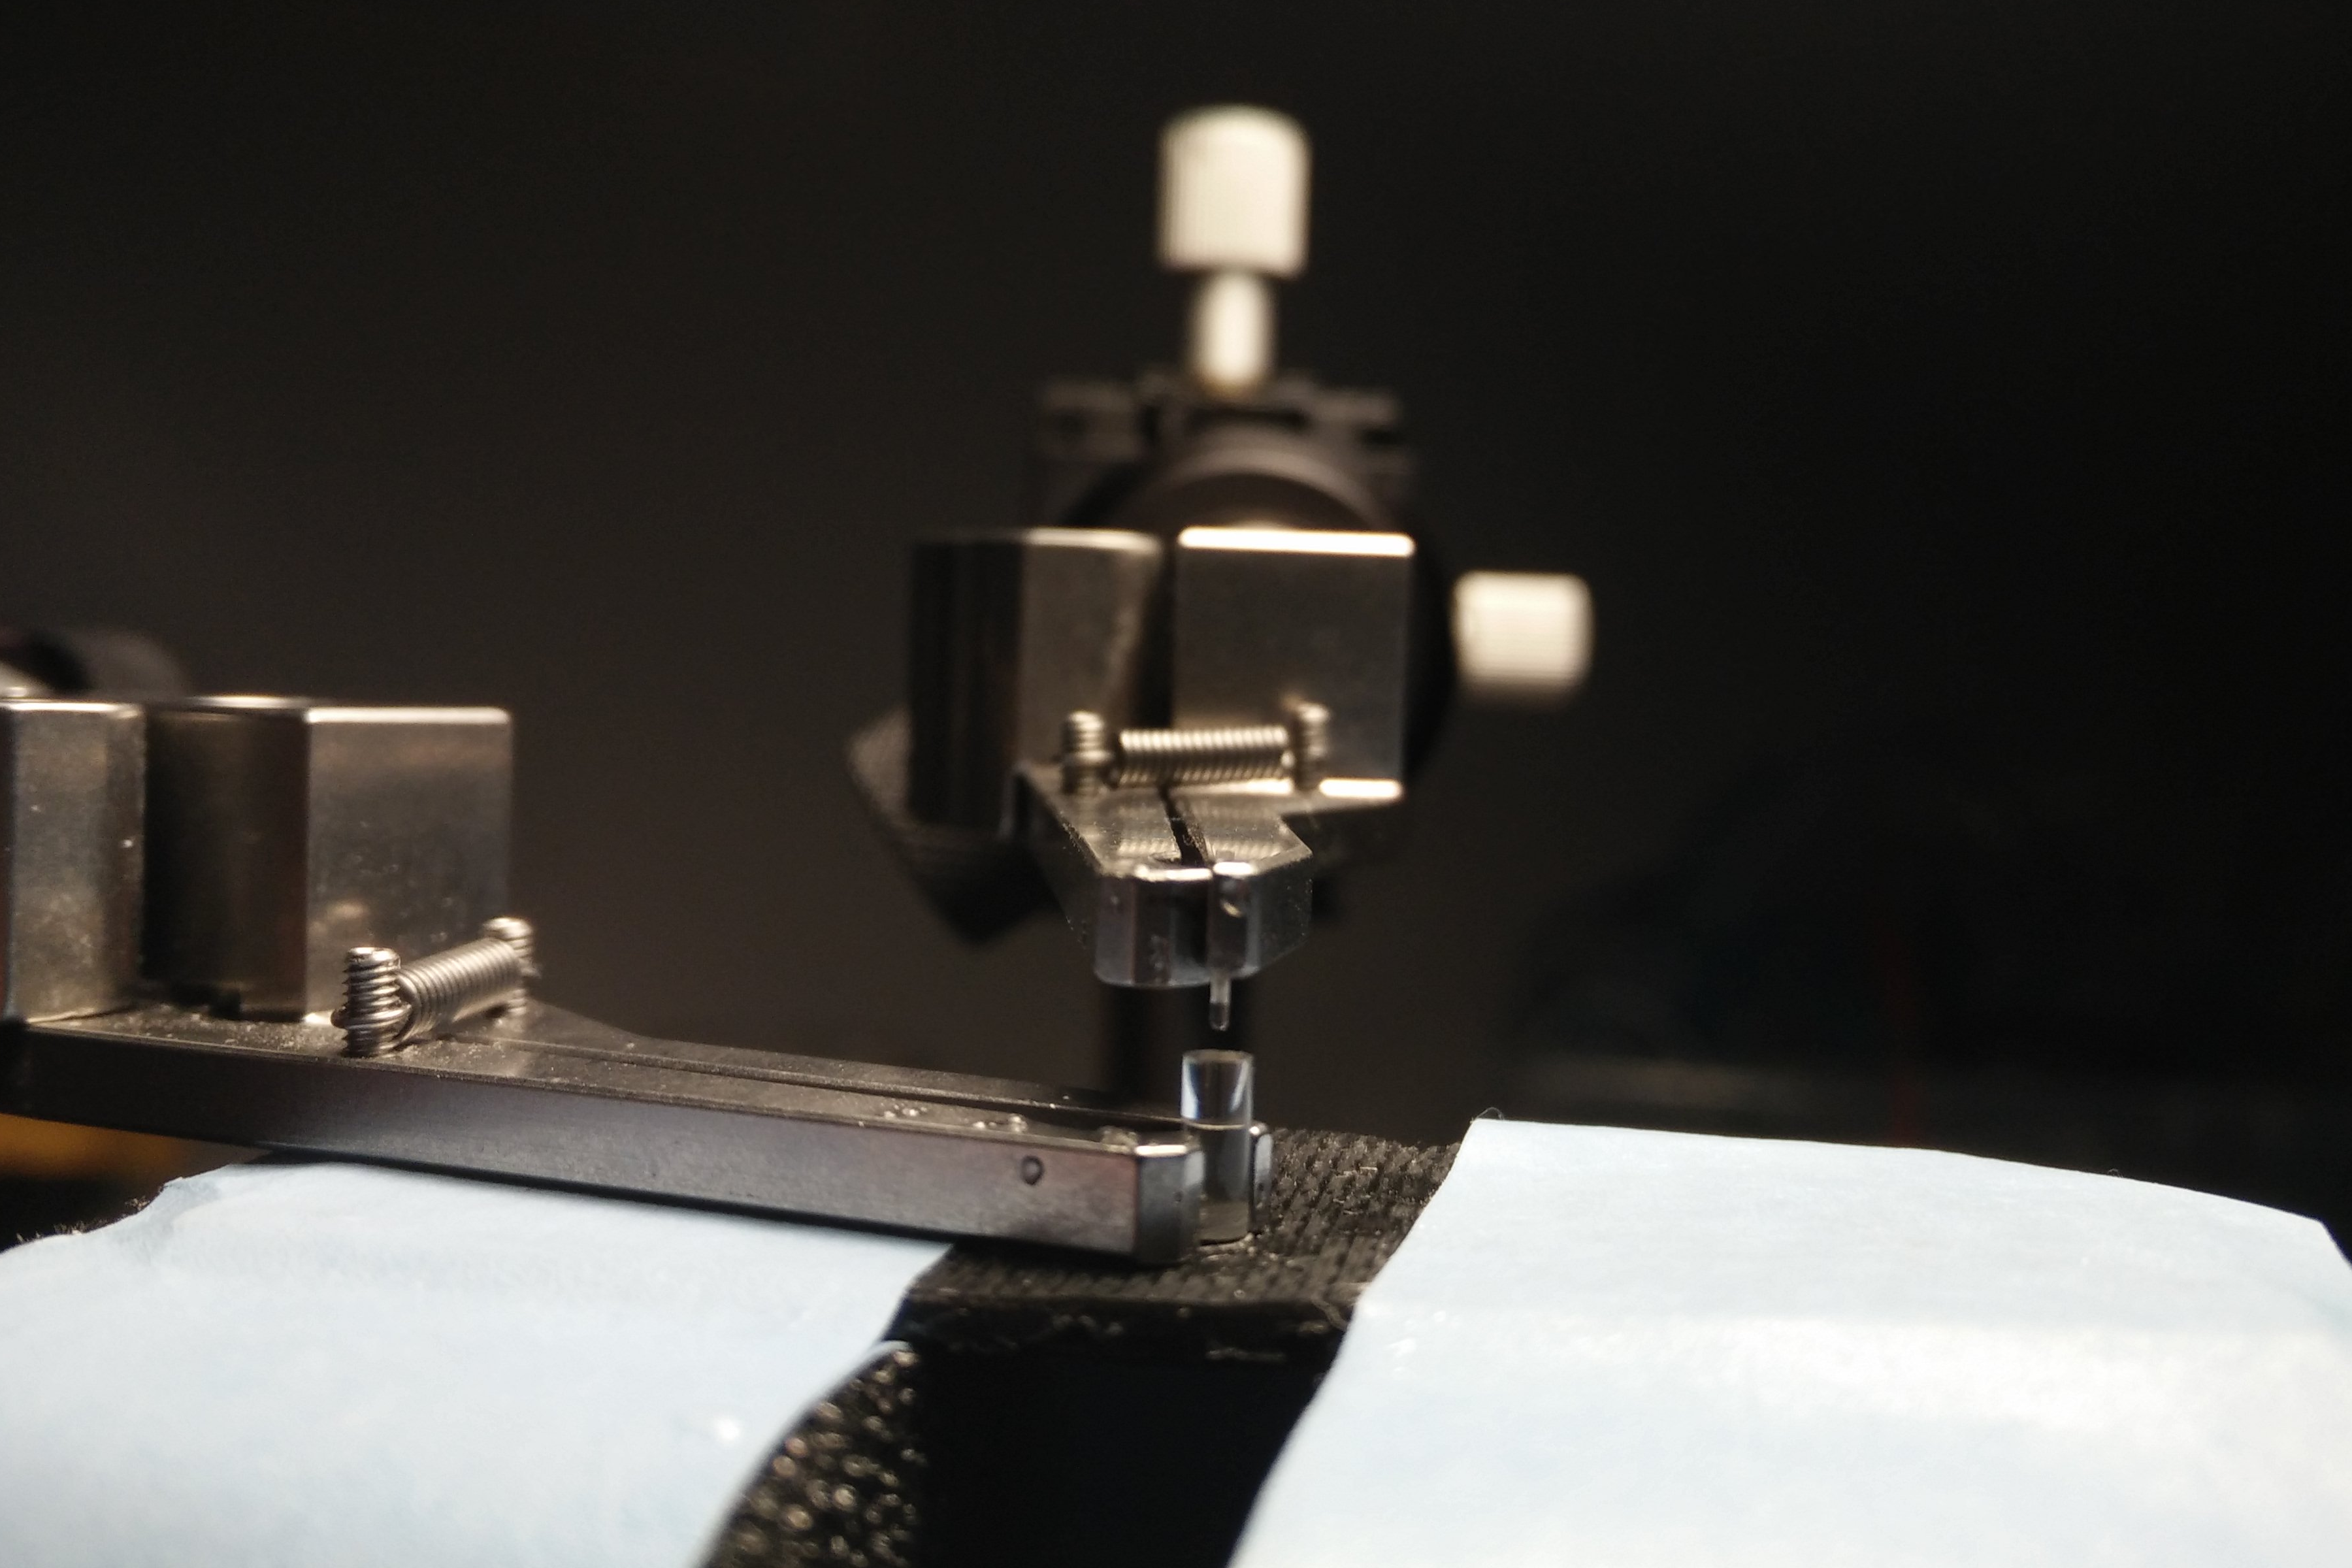
\includegraphics[width=\textwidth]{f2.png}
        \caption{\label{f.lens.2}}
    \end{subfigure}
    \begin{subfigure}[t]{.5\textwidth}
        \centering
        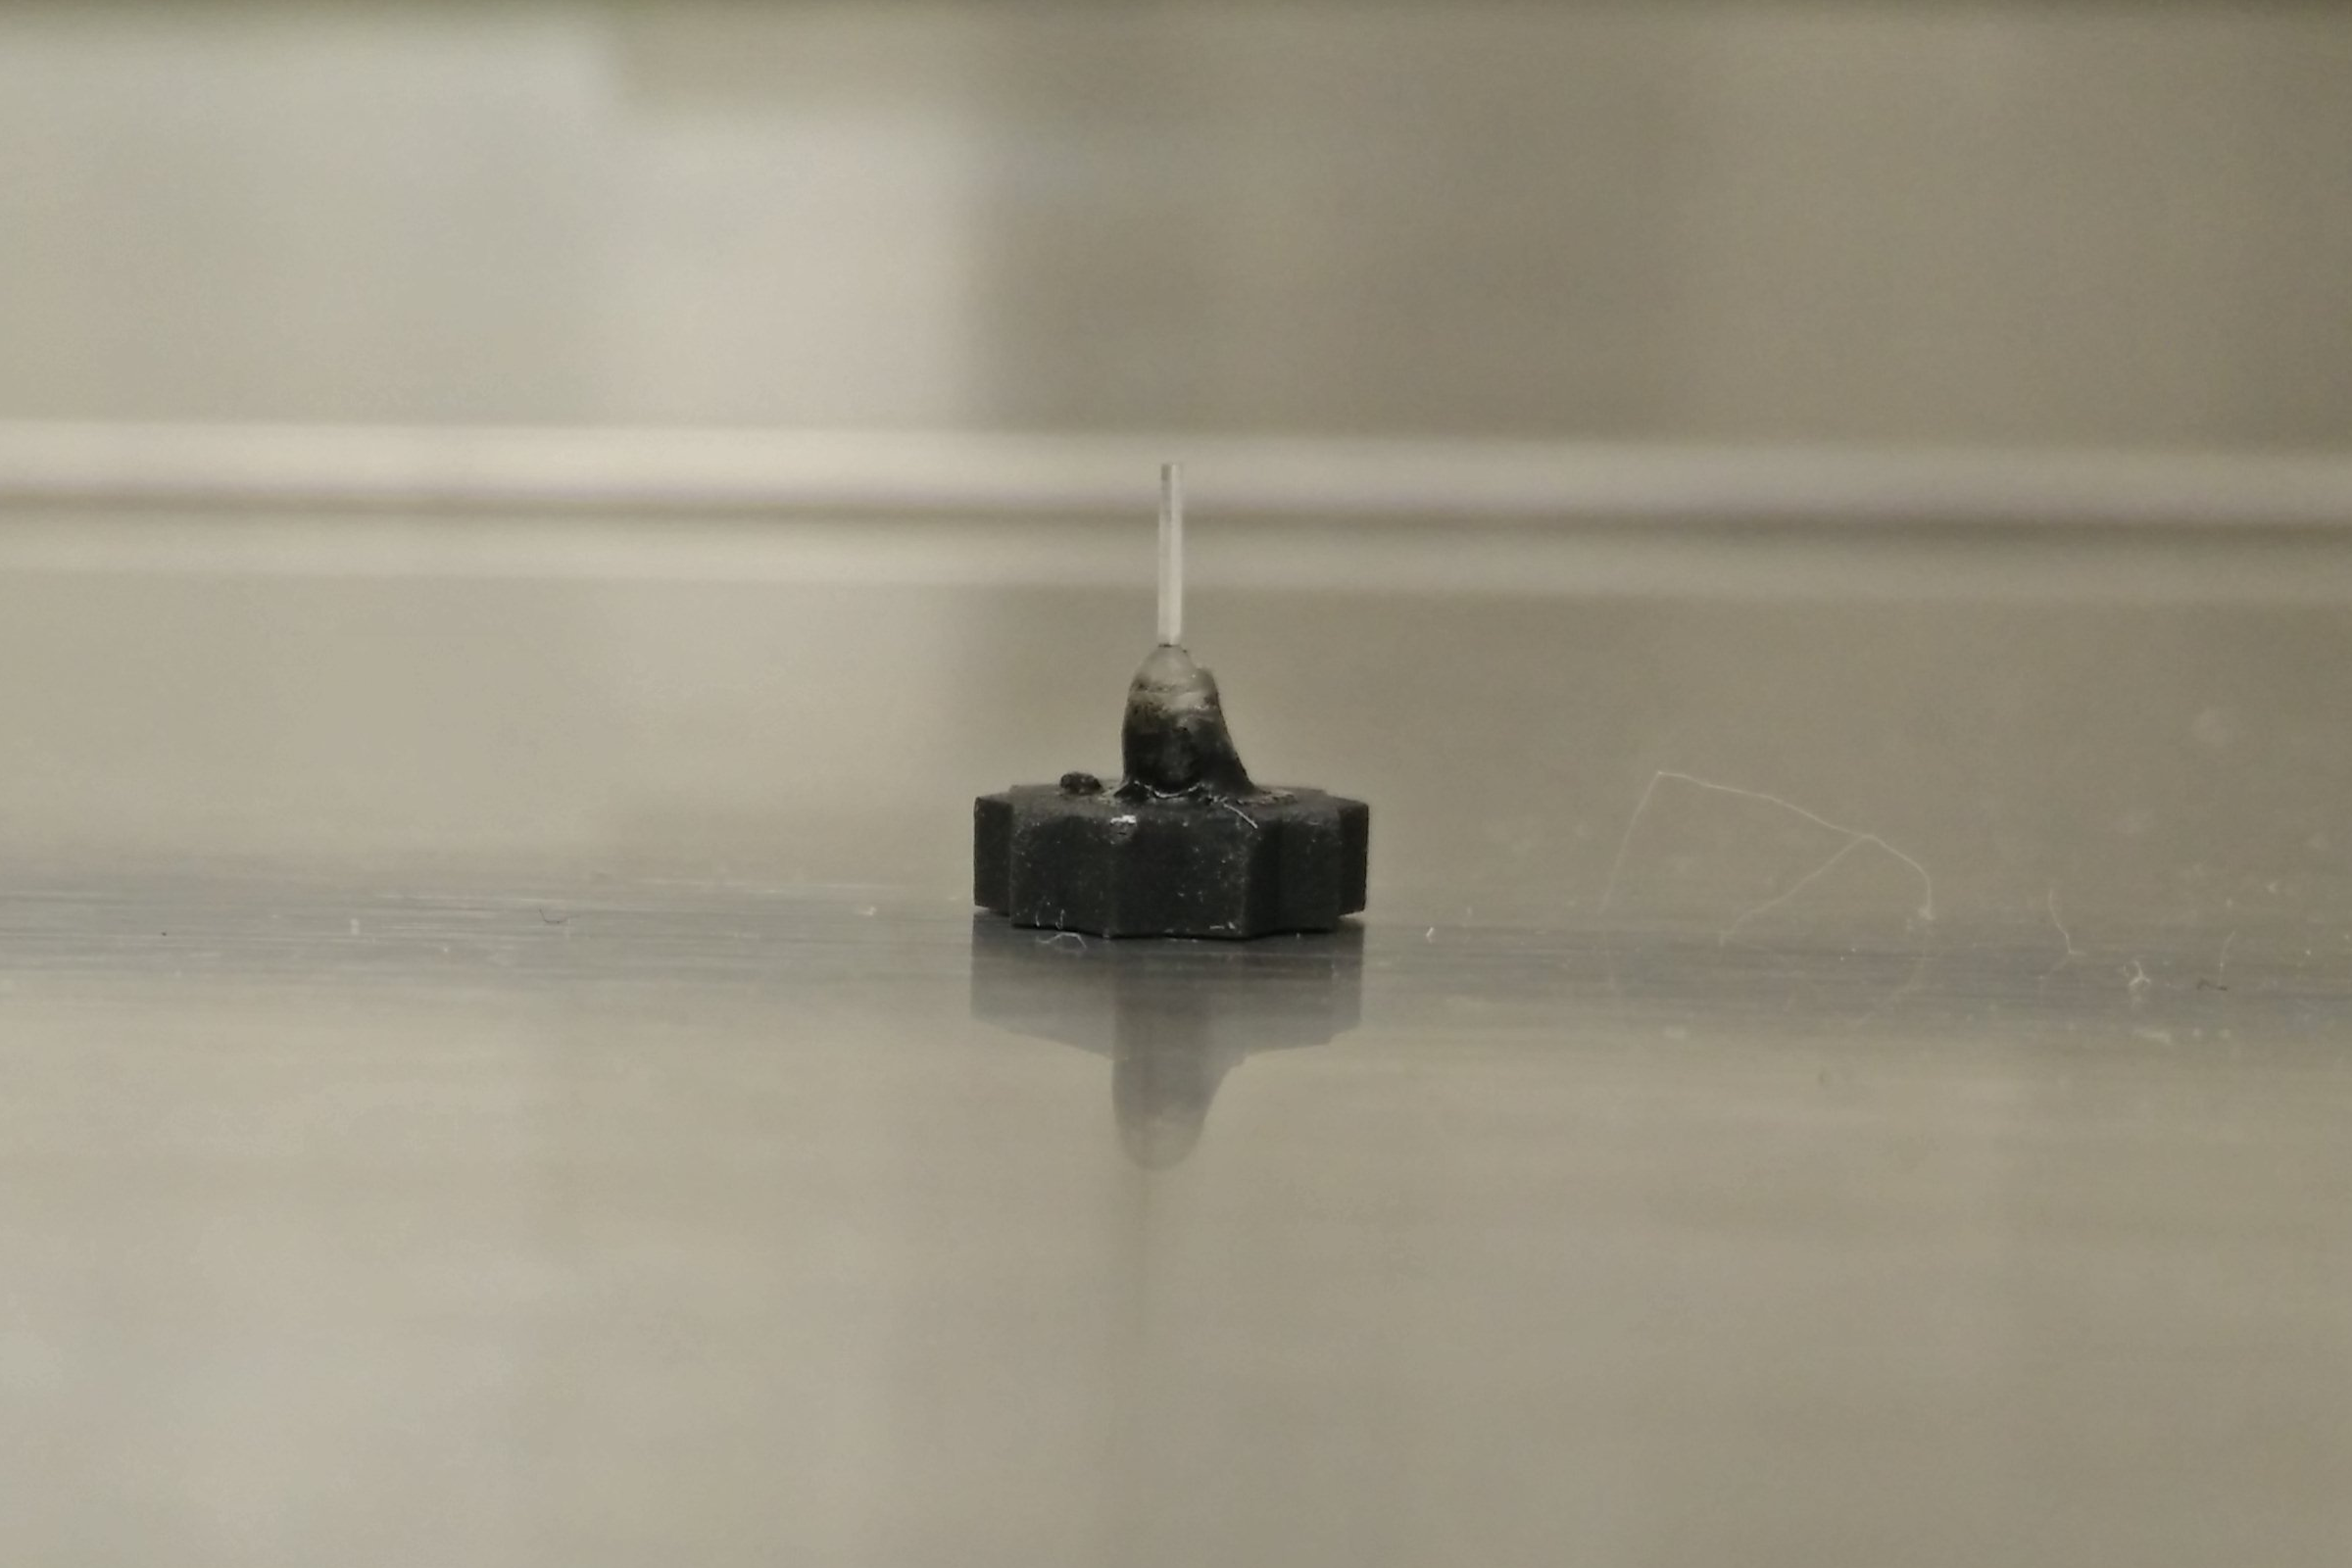
\includegraphics[width=\textwidth]{f3.png}
        \caption{\label{f.lens.3}}
    \end{subfigure}
    \caption[Assembly of deep brain imaging doublet.]{Assembly of deep brain imaging lenses. The lenses were hold by two leveled V-groove clamps. A camera was installed at the base of the large \gls{grin} lens to monitor X--Y alignment of the two lenses. Translation of the top V-groove clamp was controlled by a 3-axis manipulator. A drop of optical adhesive was placed at the bottom of the thin lens. The thin lens was then moved downwards until two lenses touch. The optical adhesive was cured by illumination of a spot \gls{uv} light source. \subref{f.lens.1} Set up for the doublet assembly. \subref{f.lens.2} Close up of the lenses in X--Y alignment. \subref{f.lens.3} Doublet assembled in a mini-microscope baseplate.\label{lens-setup}}
\end{figure}

\subsection{Viral infusion \label{viral-infusion}}

Each mouse received \gls{ip} injection of atropine (\SI{0.1}{\mg\per\kg}) and chlorohydrate (\SI{400}{\mg\per\kg}) before being secured on a stereotaxic frame. An incision was made on the scalp and the skin was pulled to the side to reveal the skull. Holes were drilled above the brain region of interest on the skull for micropipette injection. \SI{1.0}{\ul} AAV-syn-GCaMP6 virus was loaded into a glass micropipette and gradually lowered to target coordinate (\gls{ca1}: \gls{a/p} \SI{-1.8}{\mm}, \gls{m/l} \SI{1.5}{\mm}, \gls{d/v} \SI{-1.5}{\mm} from Bregma; \gls{la}: \gls{a/p} \SI{-1.4}{\mm}, \gls{m/l} \SI{3.5}{\mm}, \gls{d/v} \SI{5.0}{\mm} from Bregma), and injected at a rate of \SI{0.12}{\ul\per\min}. The micropipette was left in the brain for an extra \SI{10}{\min} before slowly retracted. The incision was sutured and treated with antibiotics. Each mouse then received subcutaneous injection of analgesic (ketoprofen, \SI{5}{\mg\per\kg}) before returned to a partially heated clean cage for recovery.

\subsection{Implantation of the mini-microscope}

Mice with viral expression of gCaMP6 were anesthetized and head-fixed in a stereotaxic frame as described in Section \ref{viral-infusion}. Three screws were placed around the viral injection site for anchoring of the microscope. For implantation targeting \gls{ca1}, a circular craniology of \SI{2}{\mm} was performed above the viral injection site. The dura was pierced and lifted with fine tweezers to expose the brain. The brain was then continually irrigated with artificial cerebral-spinal fluid to remove the blood. A 27-gauge aspiration needle was used to remove cortex and expose \gls{ca1}. For implantation targeting \gls{la}, after anchoring the screws, a 27-gauge needle was lowered to the target coordinate, left for \SI{5}{\min}, and slowly retracted to create a canal for the thin lens to implant.

The mini-microscope was then fixed on the stereotaxic frame and gradually lowered to \SI{0.2}{\mm} above the target coordinates (\gls{ca1}: \gls{a/p} \SI{-1.8}{\mm}, \gls{m/l} \SI{1.5}{\mm}, \gls{d/v} \SI{-1.3}{\mm} from Bregma; \gls{la}: \gls{a/p} \SI{-1.4}{\mm}, \gls{m/l} \SI{3.4}{\mm}, \gls{d/v} \SI{-4.8}{\mm} from Bregma). Opaque black dental acrylic was applied to secure the microscope baseplate to the skull. Once the dental acrylic was cured, the microscope body was detached from the baseplate and replaced with a cap. Mice were given \SI{5}{\mg\per\kg} ketoprofen for analgesia before returned to a clean cage for recovery.

\subsection{\textit{In vivo} mini-microscope testing}
After lens implantation, the mice were kept in the home cage for at least two weeks before the first image session. This time allows the optical window to clear. Following this recovery, the mice were handled and the cap was removed and replaced with the microscope body. A typical imaging session lasted for at least \SI{5}{\minute}. After the imaging session, the microscope body was removed, the mice were recapped and returned to their home cage.

\subsection{Image analysis}

\subsubsection{Extracting cells from calcium imaging videos}


Before processing, the raw videos were corrected for uneven illumination by applying a high-pass Gaussian filter (\SI{20 x 20}{\um} kernel) to each frame. To reduce computation time, the videos were down-sampled to 5 fps for processing. Individual cell calcium signals were extracted from the video similarly to previously described \citep{mukamel09}. First, the illumination-corrected down-sampled video was regarded as a matrix of pixels by time, and \gls{pca} was applied to reduce the temporal dimension to 300-500 components. The principal components were then regarded as mixtures of individual cells, and separated by \gls{ica}. \Gls{ica} components with a single mode and 90\% peak width of less than \SI{30}{\um} were classified as cells. The time-course of cell components were calculated by multiplying the inverse of \gls{ica} component matrix with the corresponding illumination-corrected raw video.

All calcium activity traces were normalized to have zero median and unit noise standard deviation. The noise standard deviation was estimated from median absolute deviation of the trace. The signal to noise ratio (SNR) was calculated as the ratio of maximum signal intensity and noise standard deviation. Only traces with more than 10 SNR and animals with more than 20 cells were included in the analysis. The average activity of a cell was calculated by the area under the calcium trace above 3 standard deviation of the noise divided by duration.

\subsubsection{Mapping cells across session}
Cells were extracted from the recordings for both the training and test session respectively. The position of the each cell was calculated as the center of mass of pixels above the \num{90} percentile intensity in the extracted \gls{ica} components. The position of cells for each recording were approximately aligned to have overlapping centers of mass, then rotated to have overlapping principle component vectors. The two point clouds were then precisely aligned using a manual approximation and finally \gls{trimicp} \citep{chetverikov02}. \Gls{trimicp} is robust against outliers, which allows accurate alignment even when cells were observed in one session but were missing in another. \Gls{trimicp} was performed using a \SI{40}{\percent} outlier ratio, optimizing both translation and rotation. After alignment, cells that shifted less than \SI{2}{\um} from one session to another were marked as the same cell. 


\section{Results}

\subsection{Capability and \textit{in vitro} testing of the mini-microscope}
The mini-microscope provides an easy and inexpensive tool for neuroscience laboratories to measure calcium activity in freely behaving animals. Our completely assembled mini-microscope costs less than \$\,\num{1000}, weighs less than \SI{3}{\g}, and can be bounded in a \SI{25 x 16 x 11}{\mm} box (Figure~\ref{f.scope}). Adult mice with the mini-microscope attached are able to rear, groom, and freely explore environment with no noticeable change from their natural behaviour.

The theoretical optical resolution of the mini-microscope is \SI{1}{\um}. To measure the resolution empirically, we tested the mini-microscope against \gls{usaf} resolution target (38-257, Edmund Optics). As shown in Figure~\ref{f.usaf}, the thinest lines (group 7 element 6, \SI{2.07}{\um} width) are clearly distinguishable. This suggests that the empirical resolution of the microscope is smaller than \SI{2}{\um}. With this resolution, the mini-microscope is able to resolve cell bodies and capillary blood vessels.

We first tested the mini-microscope in a perfused brain. We virally expressed \gls{gfp} in the \gls{la} of a mice using \gls{hsv}, and perfused and harvested the brain 3 days later when the \gls{gfp} expression had peaked. The brain was sliced coronally on a vibratome until fluorescence was detectable on the cutting surface. The trunk of the brain was then imaged under the mini-microscope. As seen in Figure~\ref{f.scope-gfp}, the \gls{gfp} cell bodies and the apical dendrites could be resolved from the mini-microscope image. This result confirms that the fluorescence under  \gls{led} illumination can be reliably detected by the \gls{cmos} camera.

\begin{figure}[h]
    \begin{subfigure}[t]{.3333\textwidth}
        \centering
        \input{../figs/miniscope/render.pdf_tex}
        \caption{\label{f.scope-schema}}
    \end{subfigure}
    \begin{subfigure}[t]{.6666\textwidth}
        \centering
        \input{../figs/miniscope/scope.pdf_tex}
        \caption{\label{f.scope}}
    \end{subfigure}
    \caption[Schematic of the miniature microscope.]{\subref{f.scope-schema} Schematic of the miniature microscope. Excitation light is emitted from a high-intensity blue LED, filtered and reflected to the sample by a dichroic mirror. GCaMP6 emission are collected by the gradient-index (GRIN) lens, filtered and focused onto a CMOS camera chip, where the images are sent to a computer and recorded. 
    \subref{f.scope} Assembled mini-microscope with optic path overlay. The complete mini-microscope weights less than \SI{3}{\gram} and can be bounded in a \SI{25 x 16 x 11}{\mm} box.}
\end{figure}

\begin{figure}[h]
    \begin{subfigure}[t]{.57\textwidth}
        \centering
        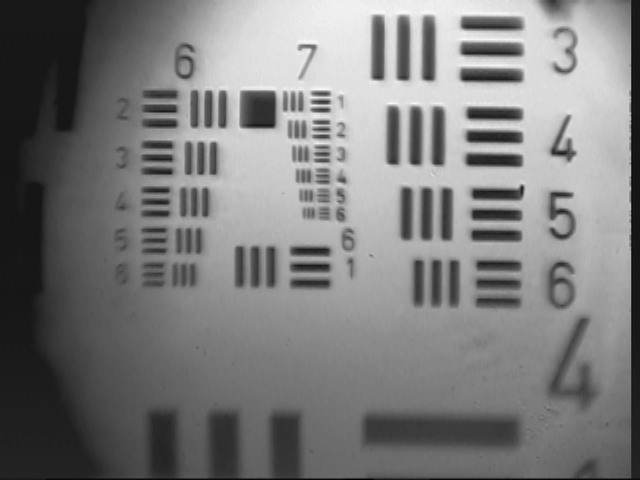
\includegraphics[width=\textwidth]{usaf-target.png}
        \caption{\label{f.usaf}}
    \end{subfigure}
    \begin{subfigure}[t]{.43\textwidth}
        \centering
        \input{../figs/miniscope/scope-gfp.pdf_tex}
        \caption{\label{f.scope-gfp}}
    \end{subfigure}
    \caption[Resolution of the mini-microscope.]{Resolution test for the mini-microscope. The mini-microscope has a resolution of less than \SI{2}{\um}, and can resolve cell bodies and apical dendrites in the perfused brain sample. 
        \subref{f.usaf} USAF resolution test target.
        \subref{f.scope-gfp} GFP-expressing cells in perfused brain.}
\end{figure}

\subsection{Measuring blood flow with mini-microscope}
To test the \textit{in vivo} imaging capabilities of the microscope, we first implanted the mini-microscope above the cortex, and injected \SI{150}{\ul} of fluorescein-dextran (molecular weight \SI{150}{\kilo\dalton}; FD150, Sigma) in the mouse tail vein. Fluorescein-dextran fills the blood vessels, and fluoresces with similar excitation and emission wavelengths to GCaMP. As expected, after fluorescein-dextran injection, the blood vessels were clearly visible when the microscope is implanted (Figure~\ref{f.bloodvessel}). The resolution of the mini-microscope allows identification of individual eurythrocytes in the capillaries, and therefore the eurythrocyte flow rate can be calculated and shown in Figure~\ref{fig.sub.vel}. This measurement allows using the mini-microscope to study haemodynamic responses in the capillaries in freely behaving mice. 
\begin{figure}[h]
    \begin{subfigure}[h]{.471\linewidth}
        \centering
        \input{../figs/miniscope/bloodvessel-raw.pdf_tex}
        \caption{\label{fig.sub.bv}}
    \end{subfigure}
    \begin{subfigure}[h]{.529\linewidth}
        \input{../figs/miniscope/bloodvessel.pdf_tex}
        \caption{\label{fig.sub.vel}}
    \end{subfigure}
    \caption[\textit{In vivo} image of blood vessels.]{\textit{In vivo} image of blood vessel. The mouse received \SI{10}{\mg\per\kg} fluorescein-dextran in tail vein. The mini-microscope was placed at cortex when the mouse was under anaesthesia. \subref{fig.sub.bv} Mean fluorescent image of blood vessels under mini-microscope. \subref{fig.sub.vel} Heatmap of eurythrocyte flow speed overlaid on the mean fluorescent image. Eurythrocyte flow speed is measured in \si{\mm\per\second}. \label{f.bloodvessel}}
\end{figure}


\subsection{Recording calcium transients in \gls{ca1}}
To test GCaMP6s expression \textit{in vivo}, we infused \gls{aav} expressing GCaMP6s into \gls{ca1} hippocampus and implanted the mini-microscope above the injection site. During the behavioural session, the mouse was placed in a novel environment to explore for \SI{5}{\minute}, during which GCaMP6 fluorescence was recorded by the mini-microscope. The maximum projection of the GCaMP6 fluorescence in a 5-minute session is shown in Figure~\ref{f.ca1bw}. We were able to extract 200 cells and their corresponding \ce{Ca^2+} transients from the recording (Figure~\ref{f.analysis}, \ref{f.ca1rainbow}).

The positions of the mouse was traced out in the behaviour video. The time-course of the identified cells was mapped back onto the behaviour of the mouse. Figure~\ref{f.traceplot} shows \ce{Ca^2+} activity of potential place cells as they responded to specific locations in the environment the mouse was in.
\begin{figure}[h]
    \centering
    \input{../figs/miniscope/cells-bw.pdf_tex}
    \caption[Image of \Gls{ca1} neurons in a freely behaving mouse.]{Cells in \gls{ca1} captured by the mini-microscope in a freely behaving mouse. Two weeks after AAV infusion and microscope implantation, the animal was allowed to freely explore a novel environment. The picture is a maximum projection of all frames captured in a 5-minute session. \label{f.ca1bw}}
\end{figure}

\begin{figure}[h]
    \centering
    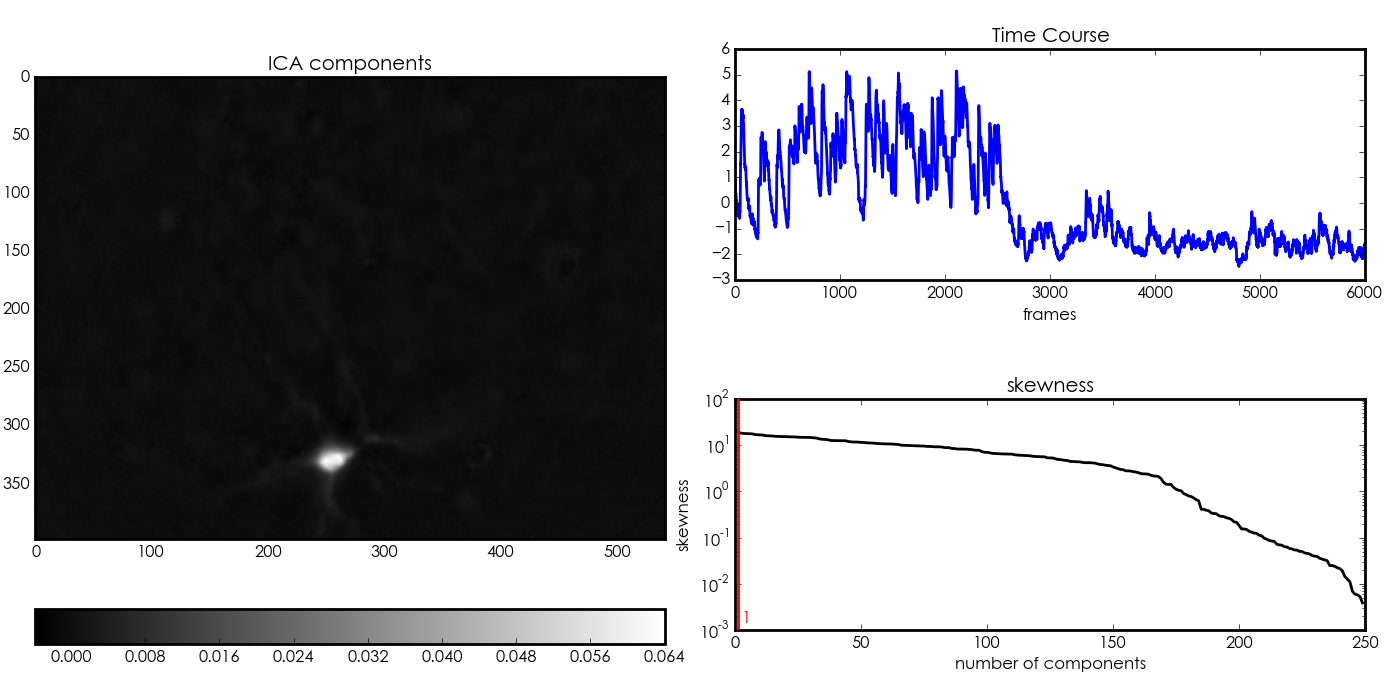
\includegraphics[width=\textwidth]{analysis1.png}
    \caption[Sample analysis data from a calcium imaging video.]{Example of an independent component of the video after analysis, showing both the extracted spatial location of the cell (left) and the un-normalized actvity (top right). \label{f.analysis}}
\end{figure}


\begin{figure}[h]
    \centering
    \input{../figs/miniscope/cells-bw-rainbow-all-final.pdf_tex}
    \caption[Cells identified in a single imaging session.]{More than 100 cells are identified in a single imaging session. The identified cells are randomly coloured. \label{f.ca1rainbow}}
\end{figure}


\begin{figure}[h]
    \begin{subfigure}[t]{.5\linewidth}
        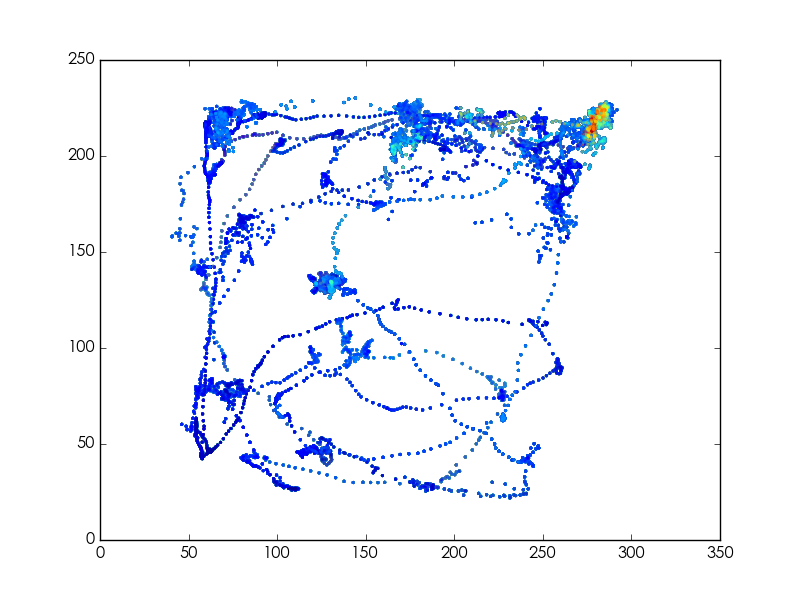
\includegraphics[width=\textwidth]{trace1.png}
    \end{subfigure}
    \begin{subfigure}[t]{.5\linewidth}
        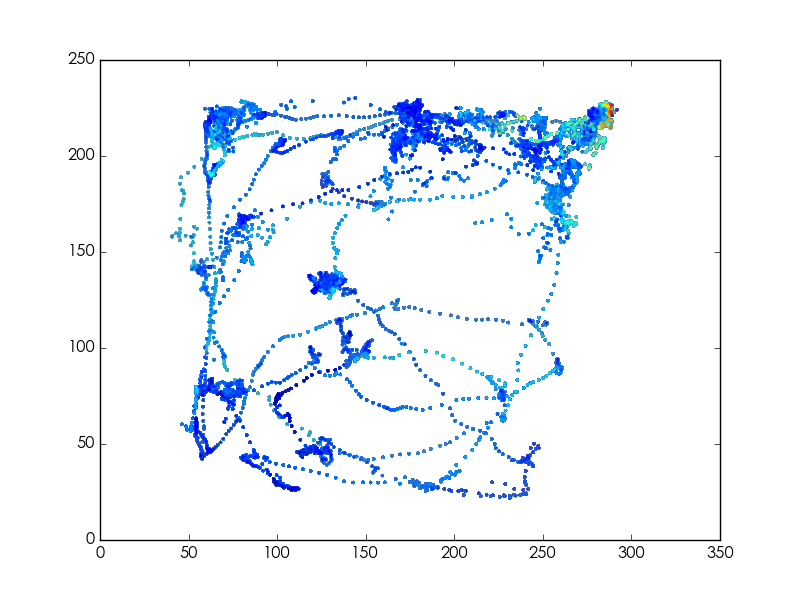
\includegraphics[width=\textwidth]{trace2.png}
    \end{subfigure}
    \begin{subfigure}[t]{.5\linewidth}
        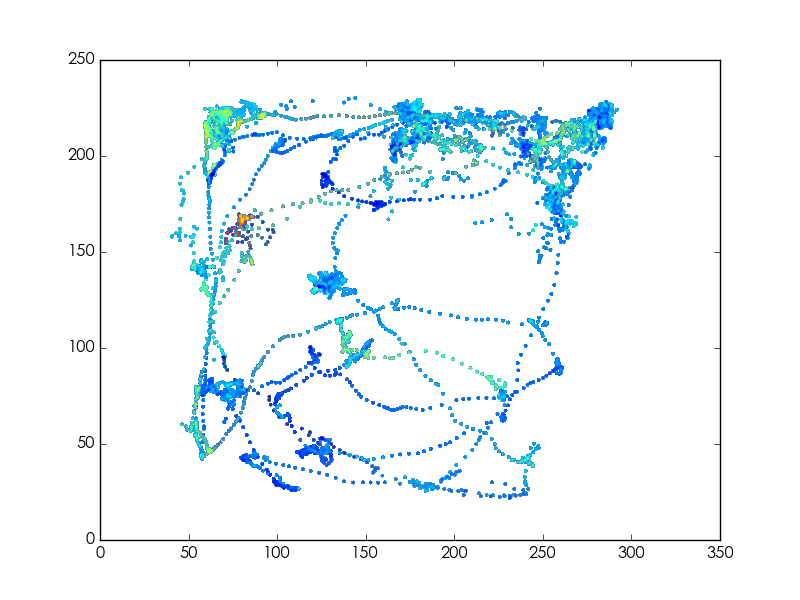
\includegraphics[width=\textwidth]{trace3.png}
    \end{subfigure}
    \begin{subfigure}[t]{.5\linewidth}
        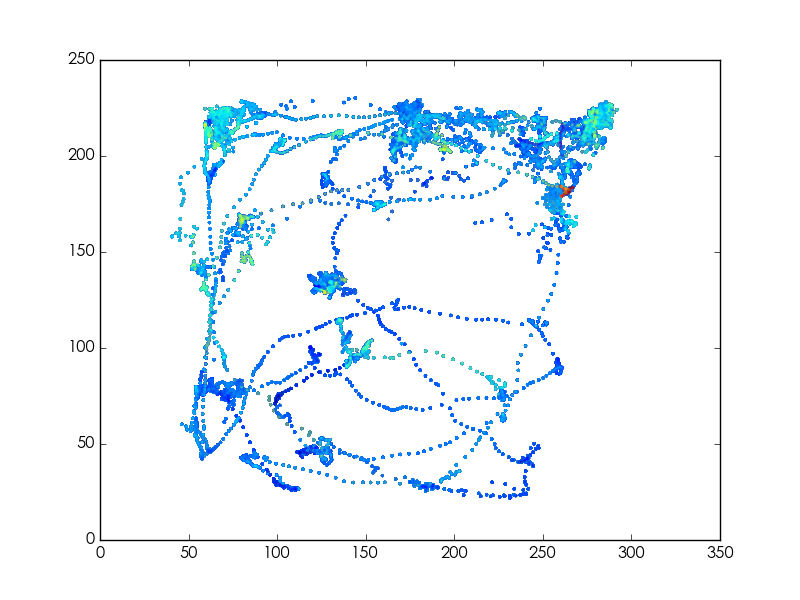
\includegraphics[width=\textwidth]{trace4.png}
    \end{subfigure}
    \caption[Detection of potential place cells in \gls{ca1} calcium imaging.]{Activity of 4 sample cells plotted against location of the mouse. The colour represents the \ce{Ca^2+} activity. The cellular activity is specific to the mouse's location in the environment. \label{f.traceplot}}
\end{figure}

\subsection{Video preprocessing}
\subsubsection{Illumination correction}
The size of the mini-microscope limits its illumination pathway, and as a result the illumination in the \gls{fov} is uneven. Uneven illumination not only affects the calcium signal and cell detection, but also adds difficulty to the motion correction step, since the uneven illumination pattern appears stable even when there is relative movement between the mini-microscope and the target. To correct this, a 2D Gaussian filter with large window (\SI{20x20}{\um}) was convolved with each frame to extract the lower frequency components of the image as the illumination pattern. The illumination pattern was then subtracted from the frame. Figure~\ref{f.illumination} shows the maximum projection of an \textit{in vivo} video recording of \gls{ca1} cells expressing gCaMP6f before and after illumination correction. Cells under intense illumination in the center can be clearly visualized after illumination correction.

\begin{figure}[h]
    \begin{subfigure}[t]{.5\textwidth}
        \centering
        \input{../figs/miniscope/illum-orig.pdf_tex}
        \caption{\label{illum.orig}}
    \end{subfigure}
    \begin{subfigure}[t]{.5\textwidth}
        \centering
        \input{../figs/miniscope/illum-corrected.pdf_tex}
        \caption{\label{illum.corrected}}
    \end{subfigure}
    \caption[Illumination correction.]{Illumination correction allows better detection of cells. This is a maximum projection of a video taken by the mini-microscope, before \subref{illum.orig} and after \subref{illum.corrected} illumination correction. Cells in the center of the \gls{fov} are clearly visible after illumination correction. \label{f.illumination}}
\end{figure}

\subsubsection{Motion correction}
After illumination correction, the video was then de-dusted and corrected for motion. Occasional dust speckles on the camera appear as stationary small dark objects in the video, and interfere with motion detection. To remove the dust speckles, pixels two standard deviation darker than mean intensity were labelled for each frame. The labelled pixels were morphologically eroded and dilated to remove labelling noise, and then inpainted using Navier-Stokes based methods \citep{bertalmio01}.

As camera motion is almost entirely translational, after dust removal we used phase correlation algorithm to achieved motion correction at sub-pixel level \citep{guizar08}. The reference frame was initialized to be the first frame. A moving average of 25 registered frames was generated, and the reference frame was updated by maximum projection of the moving average frame to the reference frame. To test the efficacy of the motion correction algorithm, we generated a recording with significant motion artifacts by loosing the connection of the mini-microscope to the baseplate during recording. As can be seen from the maximum projection of the original recording and stabilized recording (Figure~\ref{f.motion}),  we are able to obtain a stable image of cells significant motion artifacts in the original video.
\begin{figure}[h]
    \begin{subfigure}[t]{.5\textwidth}
        \centering
        \input{../figs/miniscope/shake-raw-mean.pdf_tex}
        \caption{\label{motion.orig}}
    \end{subfigure}
    \begin{subfigure}[t]{.5\textwidth}
        \centering
        \input{../figs/miniscope/shake-mean.pdf_tex}
        \caption{\label{motion.corrected}}
    \end{subfigure}
    \caption[Motion correction.]{Average video frame before and after motion correction. \label{f.motion}}
\end{figure}


\subsection{Between session stability}
To measure the stability of the imaging field between sessions, animals with gCaMP6 infused in \gls{ca1} underwent contextual fear conditioning, and \SI{24}{\hour} later, were placed back in the same context for testing. The mini-microscope was attached during both imaging sessions, and the recordings are aligned as shown in Figure \ref{f.cellalign}. In this mouse, we are able to detect 88 active cells from day 1 and 70 active cells from day 2. We were able to align videos from both sessions and found 57 cells active for both sessions. This result is similar to previously reported results \citep{ziv13}, and validates our method to map cells between sessions.

\begin{figure}[h]
    \centering
    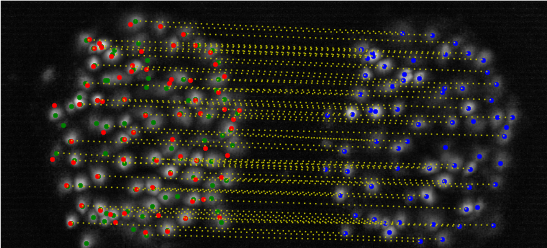
\includegraphics[width=\textwidth]{cell-align}
    \caption[Cell alignment between sessions.]{Recorded active cells in \gls{ca1} when the mouse is exposed to the same context between two days. Red and blue dots represent centroid of each recorded cell in day 1 and day 2, respectively. Yellow dotted lines shows mapping from a day 2 cell to its image in day 1 (represented with green dots). \label{f.cellalign}}
\end{figure}


\subsection{Deep brain imaging}
The original design of the miniature microscope incorporated an objective lens of \SI{1.8}{\mm} in diameter. This lens is both too thick and too short to reach deep brain structures such as \gls{la}. We modified the design and attached a \SI{4.8}{\mm} long \SI{0.5}{\mm} diameter relay \gls{grin} lens (ILW-050-P100, GoFoton) to the objective lens. Attaching the relay lens does not significantly alter the imaging ability of the mini-microscope, but allows the lens to reach deep brain regions without extensive damage. With this configuration, we were able to record neural activity form more than 40 cells in \gls{la} and track them over time (Figure~\ref{f.amygdala}).
\begin{figure}[h]
    \centering
    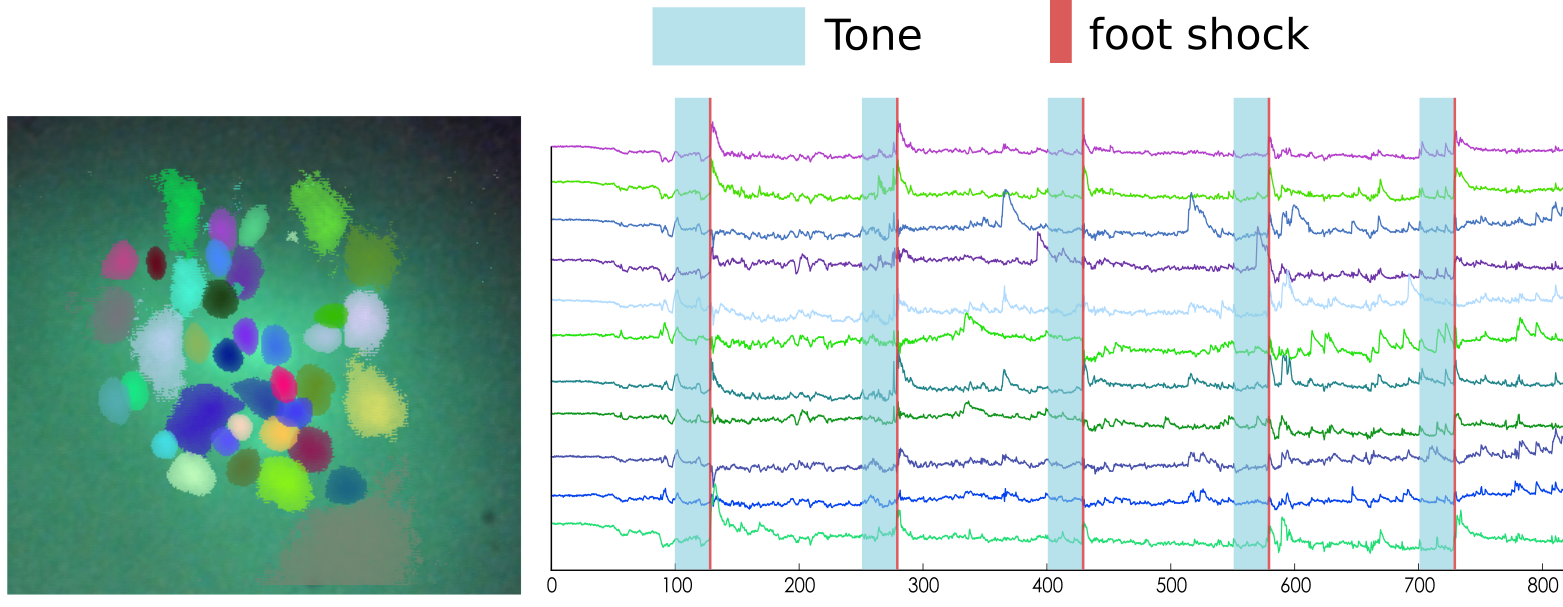
\includegraphics[width=\textwidth]{amygdala.png}
    \caption[Calcium imaging in \gls{la} during fear conditioning.]{Raw calcium signals of \gls{la} neurons during fear conditioning. Left: extracted map of neurons, randomly coloured. Right: Sample calcium signals over time.\label{f.amygdala}}

\end{figure}

\subsection{Two colour}
To test the two-colour version of the mini-microscope, we infused red retrobeads (Lumafluor) into the \gls{nac} bilaterally and gCaMP6-expressing \gls{aav} in \gls{la}. The retrobeads were trafficked retrogradely along axons, and labelled \gls{la} neurons that project to \gls{nac}. The images acquired from both the green and red channel are shown in Figure~\ref{f.twocolour.g.invivo} and \ref{f.twocolour.r.invivo}. Importantly, there is no interference between the two channels, suggesting that the two-colour mini-microscope is able to image two colour channels independently.  

\begin{figure}[h]
    \begin{subfigure}[t]{.5\linewidth}
        \input{../figs/miniscope/two-colour-g.pdf_tex}
        \caption{\label{f.twocolour.g}}
    \end{subfigure}
    \begin{subfigure}[t]{.5\linewidth}
        \input{../figs/miniscope/two-colour-r.pdf_tex}
        \caption{\label{f.twocolour.r}}
    \end{subfigure}
    \begin{subfigure}[t]{.5\linewidth}
        \input{../figs/miniscope/two-colour-green-in-vivo.pdf_tex}
        \caption{\label{f.twocolour.g.invivo}}
    \end{subfigure}
    \begin{subfigure}[t]{.5\linewidth}
        \input{../figs/miniscope/two-colour-red-in-vivo.pdf_tex}
        \caption{\label{f.twocolour.r.invivo}}
    \end{subfigure}

    \caption[Images under both green and red channel. ]{Images of cells with different fluorescent proteins using the two-colour mini-microscope prototype. \subref{f.twocolour.g} HSV-GFP in perfused brain. \subref{f.twocolour.r} HSV-tdTomato in perfused brain. \subref{f.twocolour.g.invivo} Red retrobeads \textit{in vivo} in green channel. \subref{f.twocolour.r.invivo} Red retrobeads \textit{in vivo} in red channel. \label{f.twocolour}}
\end{figure}

\section{Discussion}

In the current project, we developed a miniature integrated microscope for calcium imaging in freely behaving mice. The mini-microscope weighs less than \SI{3}{\gram}, and can be implanted on a mouse's head without altering the mouse's natural behaviour. We successfully used this microscope to record calcium transients both from \gls{ca1} in dorsal hippocampus and \gls{la}. Moreover, we added an additional red colour channel for subpopulation identification. With the additional colour channel, we have shown that it is possible to identify cells with specific projection targets by retrograde tracing using fluorescent retrobeads. 

Compared to previously designed mini-microscopes, our design is simple to build and cost efficient. All optical and electronic parts are commercially available, and the casing can be 3D-printed. The mini-microscope is designed to be easily assembled with minimal tools. Our design allows biology researchers with minimal engineering experience to build the mini-microscope and use it for biological research. Moreover, the full cost a single mini-microscope is between \$\,300 and \$\,1000, and will not represent a significant expense to most biology laboratories.

Here we used PCA--ICA for sorting the cells from videos. It is worth noting that although this method can extract cells and traces reliably, it is not optimal: the PCA--ICA method can only catch statistical regularities in the cell activity, but any spatial information is ignored. As a result, if the statistical distribution of cell activity is similar between some cells, for example if the duration of the video is relatively short or there are cells fire in synchrony, the PCA--ICA is unable to extract individual cells correctly. In addition, the results of PCA--ICA may include negative values in cell activity, which should be limited to only positive values. Recently, \citet{pnevmatikakis16} used a \gls{cnmf} approach for cell sorting from calcium imaging videos. This method took into consideration of the spatial information of each cell, as well as the activity signature of the calcium indicators, and has been shown to be more accurate than PCA--ICA in videos acquired from two-photon microscopes.  It is promising that a similar \gls{cnmf} approach can be applied to the mini-microscope dataset for cell sorting. 

Comparing to \textit{in vivo} two-photon calcium imaging, our mini-microscope lacks the advantage of focusing deeper from the \gls{grin} lens surface, as well as providing an optical slicing of the volume. The latter generates a challenge especially in cell sorting, as overlapping cells in the mini-microscope image may not be separated easily. While the \gls{pca}--\gls{ica} methods is able to resolve and distinguish partially overlapped cells \citet{mukamel09}, it is unable to distinguish two completely overlapped cells. 

Again, this limitation is can be largely resolved by \citet{pnevmatikakis16}'s \gls{cnmf} approach. They have shown that with their approach, they are able to correctly segregate and recover two overlapping cells \citep{pnevmatikakis16}. Moreover, \citet{yang16} showed that they are able to recover calcium activity recorded from simultaneous multi-plane two-photon imaging, where the cells from different z-planes are mixed together. The ability to separate overlapping cells make the \gls{cnmf} especially attractive for the mini-microscope recordings, especially in brain regions where cell density is high, and a significant portion of recorded cells overlap with each other.

In the two-colour version of the mini-microscope, colour aberration still exists, such that the alignment of the red and green channels is not perfect. However, the colour aberration is not significant, and will only result in a theoretical shift of \SI{2}{\um} in the field of view. Given that the diameter of a neuron is usually more than \SI{10}{\um}, this misalignment will not significantly affect the identification of neural subpopulations in the red channel. The colour aberration is primarily introduced by the \gls{grin} lens, and can be corrected by using a \gls{grin} lens with an optimal radial refractory index profile. However although technically possible, such \gls{grin} lens is not currently available commercially. 


\chapter{Memory formation in Alzheimer's Disease}
\section{Introduction}

\section{Material and Methods}\todo{edit methods}

\subsection{Animals and vectors}
All animals were housed in groups of 4 or 5, with a 12-hour light/dark cycle. Food and water are provided \textit{ad libitum} to all animals. Experiments were performed during the light phase of the circadian cycle. Mice were at least 8 weeks old at the beginning of all experiments. All experiments were in accordance to the Hospital for Sick Children Animal Care and Use Committee.

\subsubsection{TgCRND8 mice}
TgCRND8 mice were developed at the Center of Research for Neurodegenerative Diseases (CRND) and carry a human APP695 transgene with the Swedish (K670N-M671L) and Indiana (V717F) FAD mutations under the regulation of the Syrian hamster prion promoter \citep{chishti01}. TgCRND8 was back-crossed with C57BL/6, \gls{tg} and \gls{wt} littermates of F1 generation were used in the experiments.


\subsubsection{GP5.17 mice}
GP5.17 mice transgenically express the flourescence calcium indicator GCaMP6f under the Thy1 promoter \citep{dana14}. TgCRND8 was crossed with GP5.17. Animals that that are GCaMP6f\textsuperscript{+} and \gls{app}\textsuperscript{-}, or GCaMP6f\textsuperscript{+} and \gls{app}\textsuperscript{+} are used in the experiments. 

\subsubsection{Viral vectors}
In the TgCRND8 mice, GCaMP6f expression is delivered through \gls{aav}. GCaMP6f expression is controlled by \gls{hsyn} promoter. AAV--DJ--syn--GCaMP6f virus was purchased from Stanford University Gene and Viral Vector Core. The virus is used undiluted. 

\subsubsection{\tglu peptide}
To deliever \glu construct (YKEGYNVYG) to target, we attached it to the protein transduction domain of the \gls{hiv} \textit{tat} gene (TAT peptide). The TAT peptide is able to transport across cell membrane and \gls{bbb} through an unknown mechanism \todo{cite TAT}. The \tglu was synthesized from the sequence YGRKKRRQRRRYKEGYNVYG and desolved in saline. 


\subsection{Viral Infusion}

Each animal received \gls{ip} injection of atropine (\SI{0.1}{\mg\per\kg}) and chlorohydrate (\SI{400}{\mg\per\kg}) before being secured on a stereotaxic frame. An incision was made on the scalp and the skin was pulled to the side to reveal the skull. Holes were drilled above \gls{la} on the skull for micropipette injection. Virus was loaded into a glass micropipette and gradually lowered to target coordinate. \SI{1.5}{\ul} of virus were injected on each side at a rate of \SI{0.12}{\ul\per\min}, aiming at \gls{la} (\gls{a/p} \SI{-1.4}{\mm}, \gls{m/l} $\pm$\SI{3.5}{\mm}, \gls{d/v} \SI{5.0}{\mm} from Bregma). The micropipette was left in the brain for an extra \SI{10}{\min} before slowly retracted. The incision was sutured and treated with antibiotics. Each animal then received subcutaneous injection of analgesic (ketoprofen, \SI{5}{\mg\per\kg}) before returned to a partially heated clean cage for recovery.

\subsection{Histology}
Placement of implants and extent of viral infections was determined by \gls{gfp} expression. After all experiments, animals were transcardially perfused with first \gls{pbs} then 4\% \gls{pfa}. The brains were disected and kept in 4\% \gls{pfa} overnight, and washed with \gls{pbs}. The brains were then sliced coronally on a vibrotome (\todo{vibrotome info}) to \SI{50}{\um} thickness. Slices containing \gls{la} were then mounted on gelatin-coated glass slices with a hardening mounting media (Permaflour\todo{permaflour info}) and assessed under an epi-flourescence microscope(Nikon\todo{Nikon info}).

\subsection{Contextual fear conditioning}
Fear conditioning chambers (\SI{31 x 24 x 21}{\cm}; MED Associates, St. Albans, VT), consisted of 2 stainless steel and 2 clear acrylic walls, with a stainless steel shock-grid floor (bars \SI{3.2}{\mm} diameter, spaced \SI{7.9}{\mm} apart). A plastic drop-pan containing a 70\% ethanol solution was placed below the grid floor. A fan provided low-level white- noise during training and testing in the context. Behavior was monitored by overhead cameras, which digitized video images at \SI{15}{\Hz}. 

Animals underwent contextual fear conditioning three weeks after mini-microscope baseplate implantation. One hour before training, animals received either TAT-GluA2 peptide (i.p., \SI{15}{\mmol\per\kg}) or vehicle injection. A mini-microscope is attached to the animal to record calcium activities during both training and testing of contextual fear conditioning. During training, animals were confined in the chamber for \SI{5}{\minute}. A footshock of \SI{0.5}{\mA} was delivered at \SI{4}{\minute} time point. During testing session \SI{24}{\hour} later, animals were placed back in the training environment for \SI{10}{\minute}. 

\subsection{Animal tracing}
\todo{Animal tracing method}
Videos of animal behaviours were encoded as grey-scale images. Due to a dark background, overlaying mini-microscope wire and commutators and changing shadows, no simple feature is able to reliably identify the animal from the background. Instead, we used multiple features, calculate the distribution of the features in tracked animals, and use all the features together to estimate the position of the animal for each frame. During model fitting, distribution of every feature was estimated with a gaussian kernel \todo{kernel size}.

\subsubsection{Features}

\paragraph{Pixel intensity.} Intensity of pixel at animal's position. This feature tries to capture the animal's fur colour.

\paragraph{Normed pixel intensity.} Pixel intensity of animal's position, when the frame is normalized to zero mean and unit standard deviation. This feature tries to capture animal's fur colour with minor variations in illumination.

\paragraph{Forground pixel intensity.} Pixel intensity differenece between foreground and background images at the animal's position. The background image of the environment was generated by taking the mean pixel density across time. This feature tries to separate animals to any pixels with similar colour in the background.

\paragraph{Difference to low pass intensity.} Pixel intensity difference between foreground image and low-pass filtered foreground image (\todo{window size}) at animals position. This feature tries to capture the fact that the animal's colour is close to uniform, therefore eliminates noise pixels with similar colour.

\paragraph{Speed.} Distance between animal's positions in two consecutive frames. 

\paragraph{Change in intensity.} Difference of pixel intensity at animal's positions in two consecutive frames. This feature captures the fact that animal's colour is relative consistent between frames.

\paragraph{Chaneg in intensity (blurred).} Similar to change in intensity, but using gaussian blurred images to remove effect of random noise.

\paragraph{Magnitude of accelaration.} Magnitude of accelaration vector, which calculated as the vector difference of two consecutive velocity calculations. 

\paragraph{Segmentation area.} Edges in the frame is detected (Canny, \todo{threshold size}). The edges are then morphologically closed (\todo{iterations}) to remove sporatic edges. The area enclosing the position of the animal is then calculated. This feature tries to capture the size of the animal.


\subsubsection{Tracking}
\todo{particle filter}

For a single pixel, we calculate its score as the summation of likelihood for all the features\todo{formula}. The pixel with the highest score is the most likely position of the animal. However, calculating score for every pixel is computationally intensive. Instead, we took advantage of particle filters to estimate the distribution of score over pixels. \todo{cite particle filters, formula, detailed description}.

While improvement can still be made to this method, with the current implementation the algorithm is able to correctly track animals with minimal human intervention. \todo{ref code}


\subsection{Analysis}

\subsubsection{Cell activity}

All traces were normalized to have zero median and unit noise standard deviation. The noise standard deviation was estimated from median absolute deviation of the trace. The signal to noise ratio (SNR) were calculated as the ratio of maximum signal intensity and noise standard deviation. Only traces with more than 10 SNR and animals with more than 20 cells are included in the analysis. The average activity of a cell was calculated by the area under the calcium trace above 3 standard deviation of the noise divided by duration.

\subsubsection{Mutual information}

Freezing information and spatial information (below) were calculated according to \citet{skaggs93}. The information measurement represents how much cell activity at a single time can predict about freezing or location of the animal.  It was calculated using the following formula:

$Information = \displaystyle\sum_{i}^{}P_i  \frac{R_i}{R} log_2 \frac{R_i}{R}$

where $P_i$ represents the probability of the animal being in state $i$,  $R_i$ represents the average cell activity when the animal is in state $i$, and $R$ is the average cell activity during the session. For freezing, the states are freezing and not freezing. For spatial information, environment is divided in \num{12 x 9} grids, and the states are when animal is in one of the grids.

\subsubsection{Machine learning}

\todo{naive bayes and gSVM}

\subsubsection{Statistics}

Influence of genotype (\gls{tg}, \gls{wt}) and drug condition (vehicle, \tglu) was evaluated with two-way \gls{anova}. Covariables are controlled in a \gls{glm}. Comparisons between levels are contrasted with t-test and Bonferroni correction for multiple conparisons. Comparisons between distributions are performed using \gls{kstest}. All statistics are performed using \texttt{statsmodels} package in python.


\section{Results}


\subsection{Freezing Behaviour}
The experimental paradigm is summarized in Figure~\ref{f.ad.paradigm}. Mini-microscope baseplates were surgically implanted in \gls{ca1} hippocampus in gCaMP6f expressing \gls{wt} and \gls{tg} animals. To transiently increase surface GluA2 density, we used a short interference peptide (\tglu) to block GluA2-containing \gls{ampar} endocytosis. The animals received either vehicle (Veh) or \tglu{} (Glu) peptide one hour before training. Twenty-four hours later, the animals were tested in the training chamber. Calcium transients were recorded during both training and testing session of contextual fear conditioning. Figure~\ref{f.ad.trace} shows cells recorded from a single animal and a sample of calcium traces. 
\begin{figure}[h]
    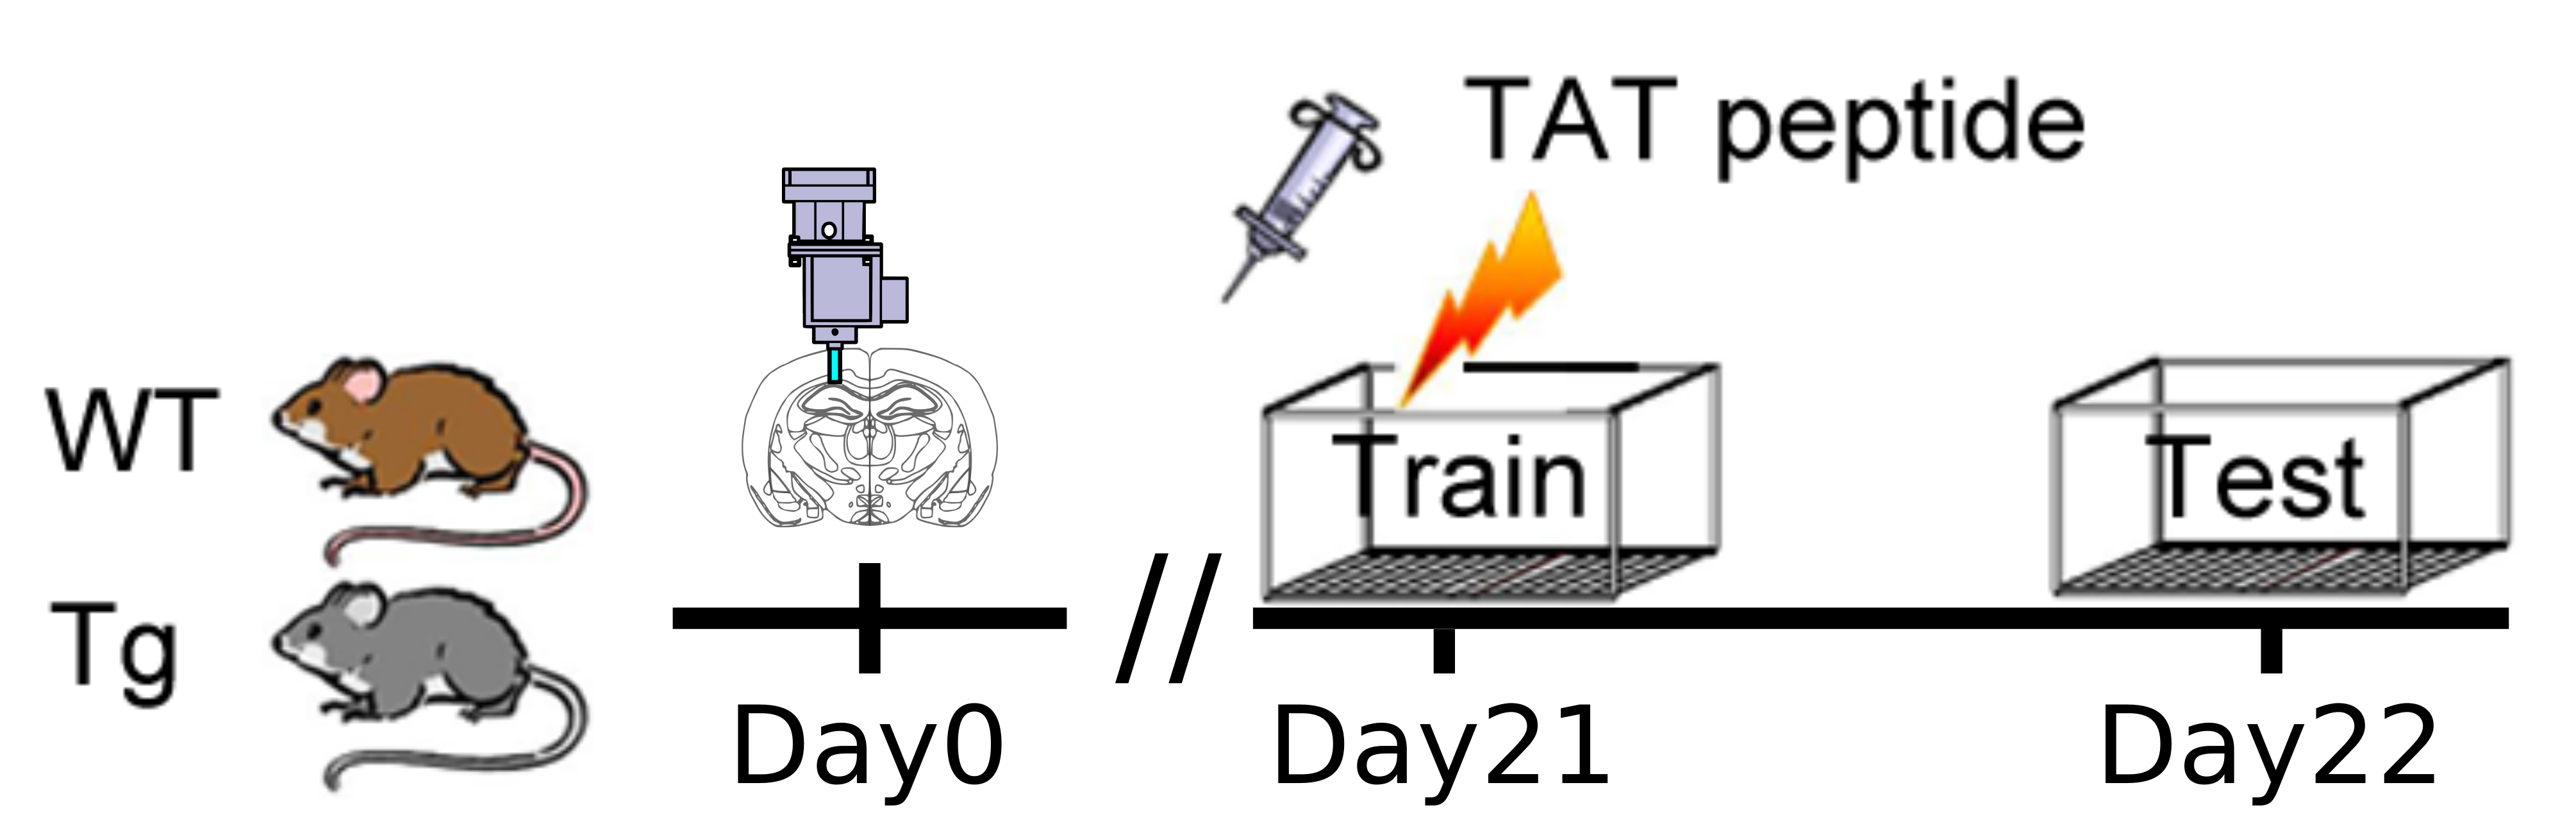
\includegraphics[width=\textwidth]{paradigm.png}
    \caption{Experimental paradigm. Adult \gls{wt} and \gls{tg} animals (with gCaMP6f expression) were implanted with a mini-microscope baseplate targeting CA1 hippocampus on day 0. The cells were visible three weeks later. Animals received \tglu peptide (i.p.) \SI{1}{\hour} before contextual fear conditioning. Animals were tested \SI{24}{\hour} later for freezing behaviour. Calcium activity were recorded for both training and testing session. \label{f.ad.paradigm}}
\end{figure}

\begin{figure}[h]
    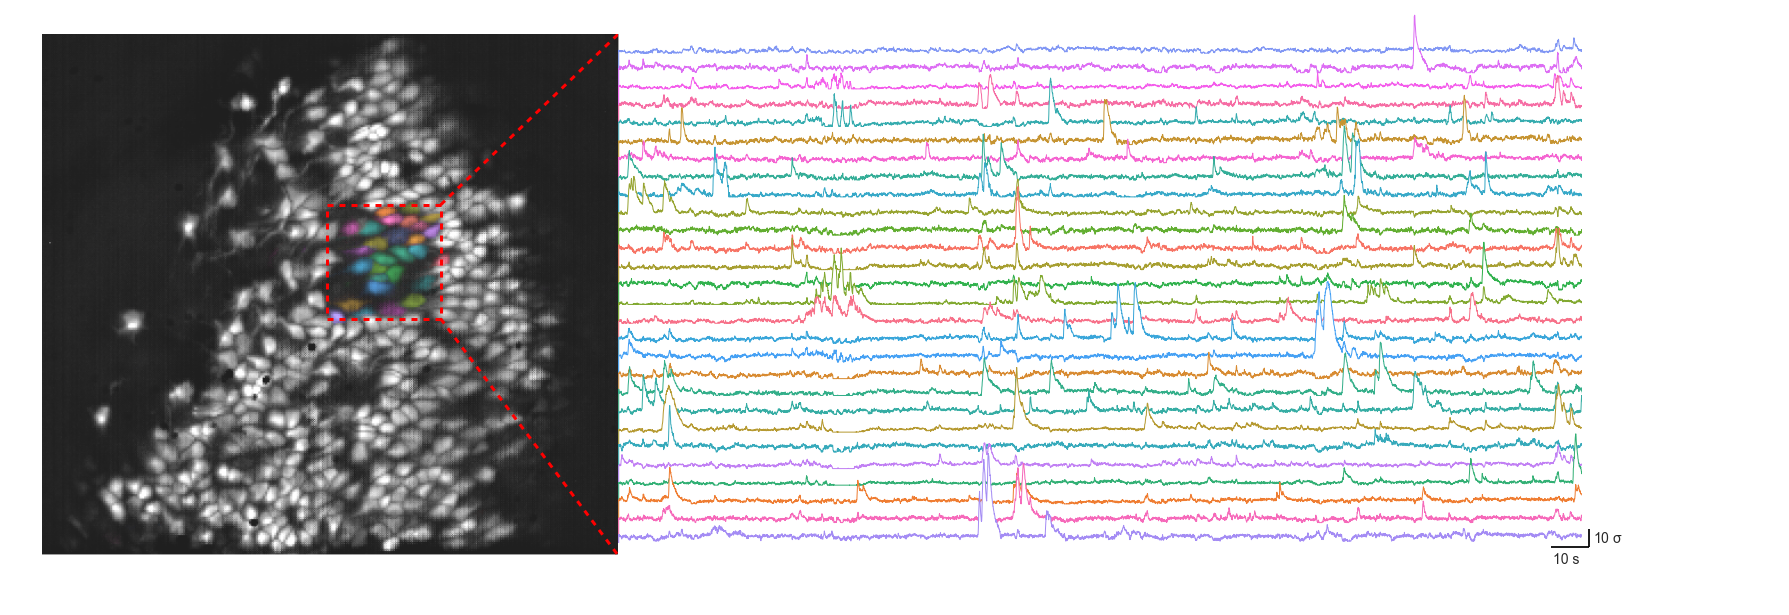
\includegraphics[width=\textwidth]{trace.png}
    \caption{Sample cell image and traces. Traces are random coloured and correspond to cells of the same colour. \label{f.ad.trace}}
\end{figure}

Figure~\ref{f.ad.freezing} shows the percent of freezing during testing. Two-way \gls{anova} has revealed significant main effect in genotype (F\tsb{1,27}=12.79, p=0.001) as well as a significant interaction between genotype and treatment (F\tsb{1,27}=5.45, p=0.027). Posthoc tests show that \gls{tg} animals have significant lower freezing (\gls{wt}-Veh vs \gls{tg}-Veh, T=4.21, p<0.001), and this effect is fully rescued by \tglu treatment (\gls{tg}-\tglu vs \gls{tg}-Veh, T=2.85, p=0.008; \gls{wt}-Veh vs \gls{tg}-\tglu, T=1.12, P=0.27). \tglu has no significant effect on \gls{wt} animals (\gls{wt}-Veh vs \gls{wt}-\tglu, T=0.355, p=0.72). This result is consistent with our hypothesis, Tg animals showed decreased freezing, and this was rescued by \tglu treatment. 

\todo{freezing}
\begin{figure}[h]
    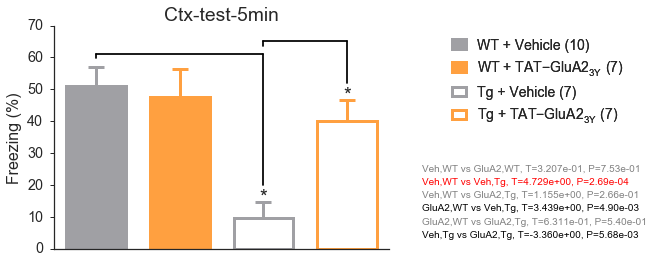
\includegraphics[width=\textwidth]{freezing.png}
    \caption{Percent of freezing during testing. \Gls{tg} animals have significant lower freezing, and \tglu treatment returns the freezing to wildtype level. \label{f.ad.freezing}}
\end{figure}



\subsection{\tglu rescues hyperactivity in \gls{tg} cells}

Figure~\ref{f.ad.acttrain} shows average cell activity during training session before footshock is delivered. During training, two-way \gls{anova} reveals significant major effects of genotype (F\tsb{1,3033}=6.2, p=0.01) and treatment (F\tsb{1,3033}=5.1, p=0.02) as well as a significant interaction between genotype and treament (F\tsb{1,3033}=7.7, p=0.006). Posthoc tests shows that \gls{tg}-Veh has significantly higher cell activity (WT-Veh vs Tg-Veh, T=-3.72, p<0.001), and \tglu treatment is able to restore average cell activity to \gls{wt} level. (Tg-\tglu vs Tg-Veh, T=-3.58, p<0.001; WT-Veh vs Tg-\tglu, T=0.14, p=0.89). \tglu does not have any effect on \gls{wt} animals (WT-Veh vs WT-\tglu, T=-0.137, p=0.89) This result is consistent with previous reports in the literature \citep{verret12}, showing cells in Tg animals have increase overall cell activity. Interestingly, while \tglu treatment restores the the mean cell activity during training, the distribution of cell activity is significantly different from \gls{wt} (WT-Veh vs Tg-\tglu, K=0.16, P<0.001). As is shown in the cumulative distribution plot, Tg-\tglu still have a over-proportion of highly active cells. 
\todo{Discuss: \tglu is not able to rescue cells with very high activity}

Similar effect were found during testing (Figure~\ref{f.ad.acttest}). Two-way \gls{anova} revealled significant major effect of genotype (F\tsb{1,3029}=32.7, p<0.001) and treatment (F\tsb{1,3029}=27.4, p<0.001), as well as their interaction (F\tsb{1,3029}=78.4, p<0.001). Post-hoc tests show significant increase of cell activity in Tg-Veh group (WT-Veh vs Tg-Veh, T=-10.1, p<0.001), and this effect is corrected by \tglu treament (WT-Veh vs Tg-\tglu, T=0.73, p=0.47; Tg-\tglu vs Tg-Veh, T=-9.97, p<0.001). There is also a trend of increase in cell activity after \tglu treatment in \gls{wt} group, however the p-value is close to threshold after correction of multiple comparison (WT-Veh vs WT-\tglu, T=-2.53, p=0.012, threshold = 0.013). Interestingly during testing, \tglu is able to fully rescue the hyper-activity in \gls{tg} group (\gls{kstest}: Veh-WT vs Tg-\tglu, K=0.06, p=0.07; Tg-Veh vs Tg-\tglu, K=2.29, p<0.001). These results suggest that the rescuing effect of \tglu in \gls{tg} animals is slow and long-lasting.

\begin{figure}[h]
    \begin{subfigure}[h]{\textwidth}
        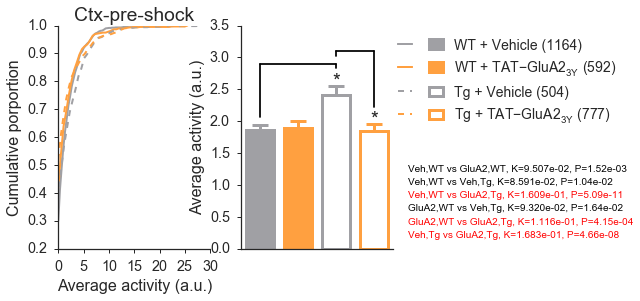
\includegraphics[width=\textwidth]{activity_train.png}
        \caption{\label{f.ad.acttrain}}
    \end{subfigure}
    \begin{subfigure}[h]{\textwidth}
        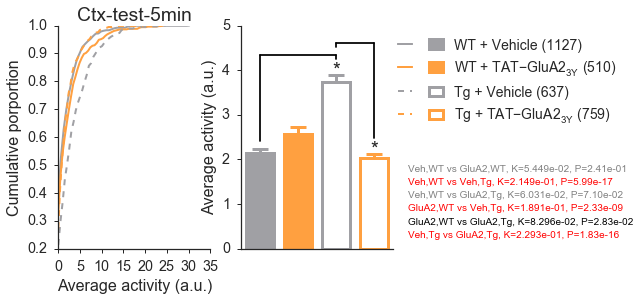
\includegraphics[width=\textwidth]{activity_test.png}
        \caption{\label{f.ad.acttest}}
    \end{subfigure}
    \caption{Distribution and mean of average cell activity during \subref{f.ad.acttrain} training and \subref{f.ad.acttest} testing. Cells in the Tg animals are significantly more active, and this is rescued by \tglu treatment. \label{f.ad.activity}}
\end{figure}

\subsection{\tglu rescues freezing encoding deficit in \gls{tg} cells}

We then investigated that how \gls{wt} and \gls{tg} cells encodes freezing. First we looked at cells individually, and calculated the mutual information between cell firing and freezing \citep{skaggs93}. This measurement reflects how much prediction power a cell has for freezing in a period of time. The group differences in freezing information is then compared using two-way \gls{anova}. There is significant main effect in both genotype (F\tsb{1,4380}=114.8, p<0.001) and treatment (F\tsb{1,4380}=7.3, p=0.007), and a significant interaction between the two factors (F\tsb{1,4380}=33.8, p<0.001). Posthoc tests show Tg-Veh group has significantly less freezing information (WT-Veh vs Tg-Veh, T=11.8, p<0.001), and this deficit is partially rescued by \tglu treatment (Tg-\tglu vs Tg-Veh, T=6.05, p<0.001), as there is a trend that Tg-\tglu group has less freezing information than WT-Veh group (WT-Veh vs Tg-\tglu, T=2.12, p=0.03, threshold=0.0125; Figure~\ref{f.ad.freeze_info}). This result suggests in the \gls{tg} group, the cell activity in hippocampus \gls{ca1} does not predict the animal's behaviour well, however this is improved with \tglu treatment but not fully rescued. 
\begin{figure}[h]
    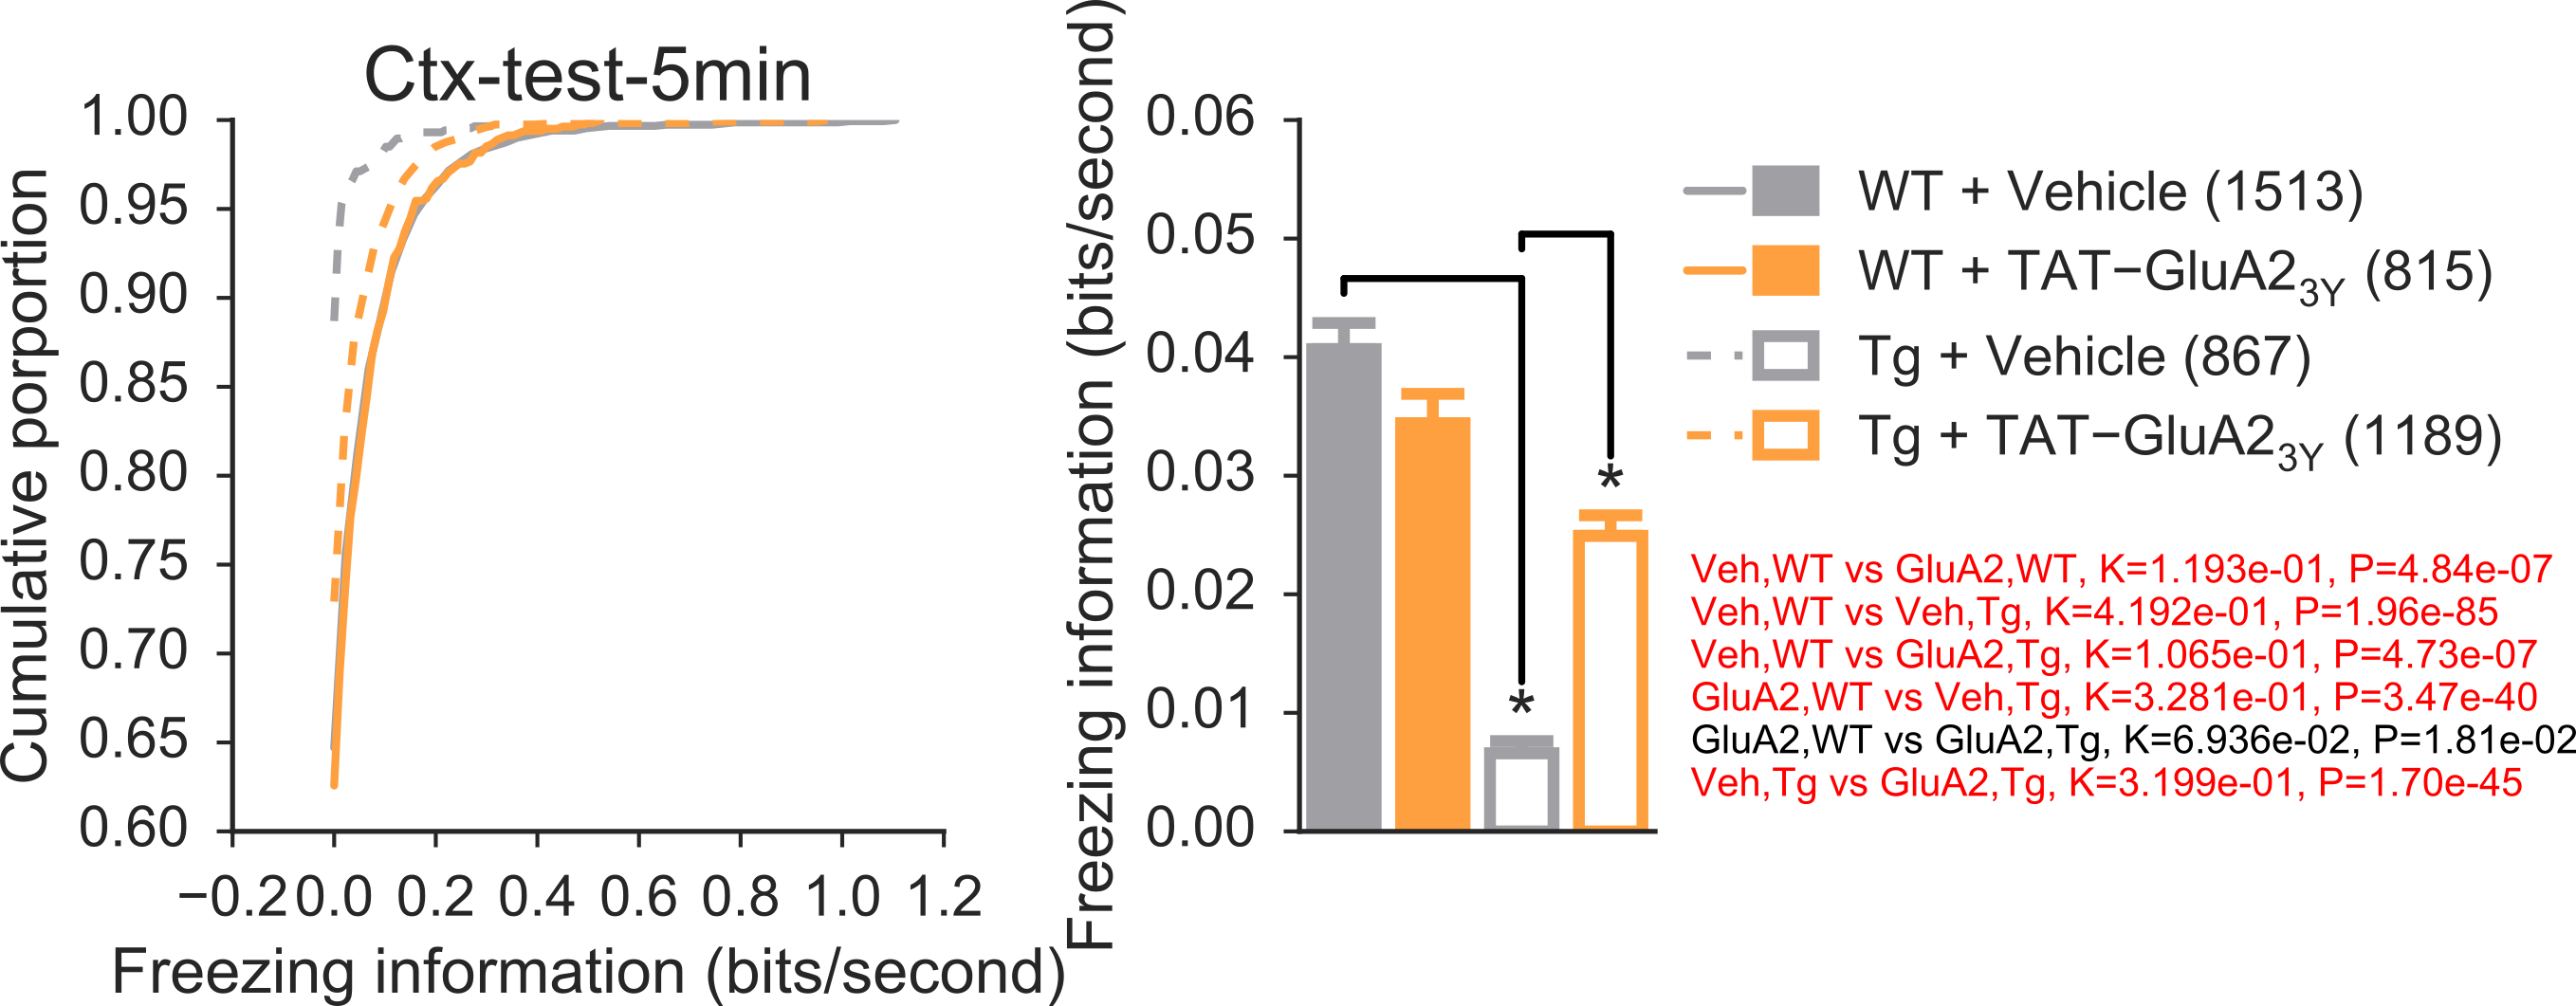
\includegraphics[width=\textwidth]{freeze_info.png}
    \caption{Freezing information during testing. This measurement represent how much information a cell have in a period of time about whether the animal is freezing. Cells in \gls{tg} animals encode significantly less freezing than the \gls{wt} groups, and \tglu treatment can only partially rescue the effect. \label{f.ad.freeze_info}}
\end{figure}
    

Then using machine learning methods, we investigated how freezing is encoded at a network level by training general classifiers to predict animals' behaviour from recorded cell activity. Both approach suggest that Tg animals have consistent worse freezing encoding both at a cellular level but also at a network level. 

While all the measurements we have performed considers each cell individually, are the cells independent of each other, or is part of the information encoded in the coordination between them? To answer this question, we have build two classifiers: a \gls{nbc} which models the cells independent of each other, and a \gls{gsvm}, which also uses the dependency between cells for prediction. The result is shown in Figure~\ref{f.ad.classifier}. 

A three-way \gls{anova} of genotype * treatment * classifier was carried out. There are significant main effect of genotype (F\tsb{1,50}=17.2, p<0.001) and classifier (F\tsb{1,50}=14.4, p<0.001),
The \gls{gsvm} significantly outperforms the \gls{nbc} classifier, suggesting that the network encodes more information than the cells individually. Moreover, both classifiers perform significantly worse in the Tg group, further supports our hypothesis that Tg animals have inferior fear memory encoding.
\begin{figure}[h]
    \begin{subfigure}[h]{\textwidth}
        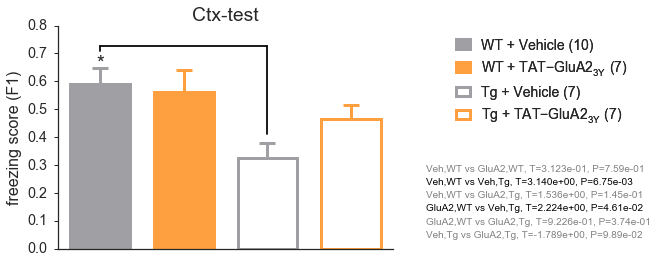
\includegraphics[width=\textwidth]{nb.png}
        \caption{\label{f.ad.nb}}
    \end{subfigure}
    \begin{subfigure}[h]{\textwidth}
        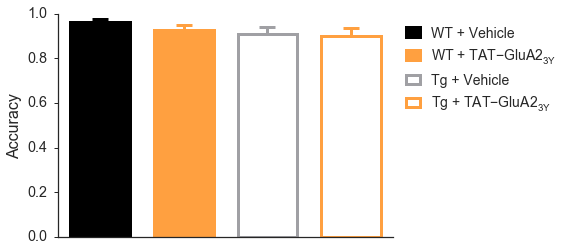
\includegraphics[width=\textwidth]{svm.png}
        \caption{\label{f.ad.svm}}
    \end{subfigure}
    \caption{Performance of \subref{f.ad.nb} \gls{nbc} and \subref{f.ad.svm} \gls{gsvm} in predicting freezing from cell activity. Results are measured as F1 score. Both classifiers showed inferior performance in \gls{tg} group, further supports the hypothesis that \gls{tg} animals have sub-optimal freezing encoding. Interestingly, since \gls{nbc} assumes the cells are independent and \gls{gsvm} is more general, the performance difference between the two suggest a portion of freezing information is encoded in the coordination between the activity of the cells. \label{f.ad.classifier}}
\end{figure}




\subsection{Difference of encoding in \gls{tg} animals is not a result of animal's behaviour}

However, given that the Tg animals also show behavioural difference, we then try to answer the question: is the difference in neural coding inherit of the Alzheimer animal, or a result of the different behaviour? Given that CA1 cells are known to represent place, we have calculated the freezing information marginalized over all animal positions, therefore eliminating it's effect in the calculation of freezing information. The result is similar and shown in Figure~\ref{f.ad.freeze_ctrl}.  
\begin{figure}[h]
    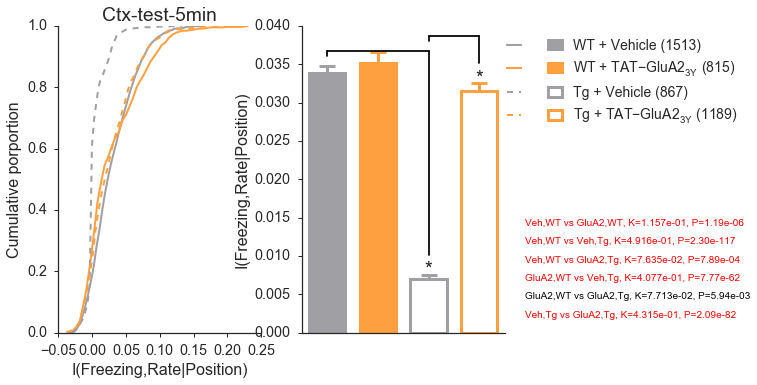
\includegraphics[width=\textwidth]{freeze_position.png}
    \caption{Freezing information conditioned on animal's position. This measurement removes the effect of position from freezing information measurement. Two-way \gls{anova} shows significant main effects in genotype (F\tsb{1,4380}=112.8, p<0.001) and treatment (F\tsb{1,4380}=30.4, p<0.001), as well as significant interaction between the two factors (F\tsb{1,4380}=48.6, p<0.001). Posthoc tests show that Tg-Veh has significant lower freezing information with position controlled (WT-Veh vs Tg-Veh, T=12.5, p<0.001), and partially rescued by \tglu (Tg-\tglu vs Tg-Veh, t=8.85, p<0.001; WT-Veh vs Tg-\tglu, t=3.56, p<0.001). This result is similar to Figure~\ref{f.ad.freeze_info}. This suggest that the position of the animal is not a confounding factor for freezing information measurement. \label{f.ad.freeze_ctrl}}
\end{figure}


In addition, we also checked whether the freezing information coding is a result of different freezing or uneven spatial coverage of the behavioural chamber, which are represented by freezing entropy and spatial entropy respectively. To check these two factors, we have pooled the groups with similar behaviour (\gls{wt}, \gls{wt}-\tglu, \gls{tg}-\tglu), and correlated percent freezing, freezing entropy, total distance and spatial entropy against freezing information within the pooled groups. If the behavioural measurement have no influence in the freezing information, we would expect no correlation. Indeed, that is what we have found in Figure~\ref{f.ad.corrs}. These control measurements have shown that the reduction of freezing encoding in the Tg animals is not affected by the difference in the animals' behaviour.
\begin{figure}[h]
    \begin{subfigure}[t]{.5\textwidth}
        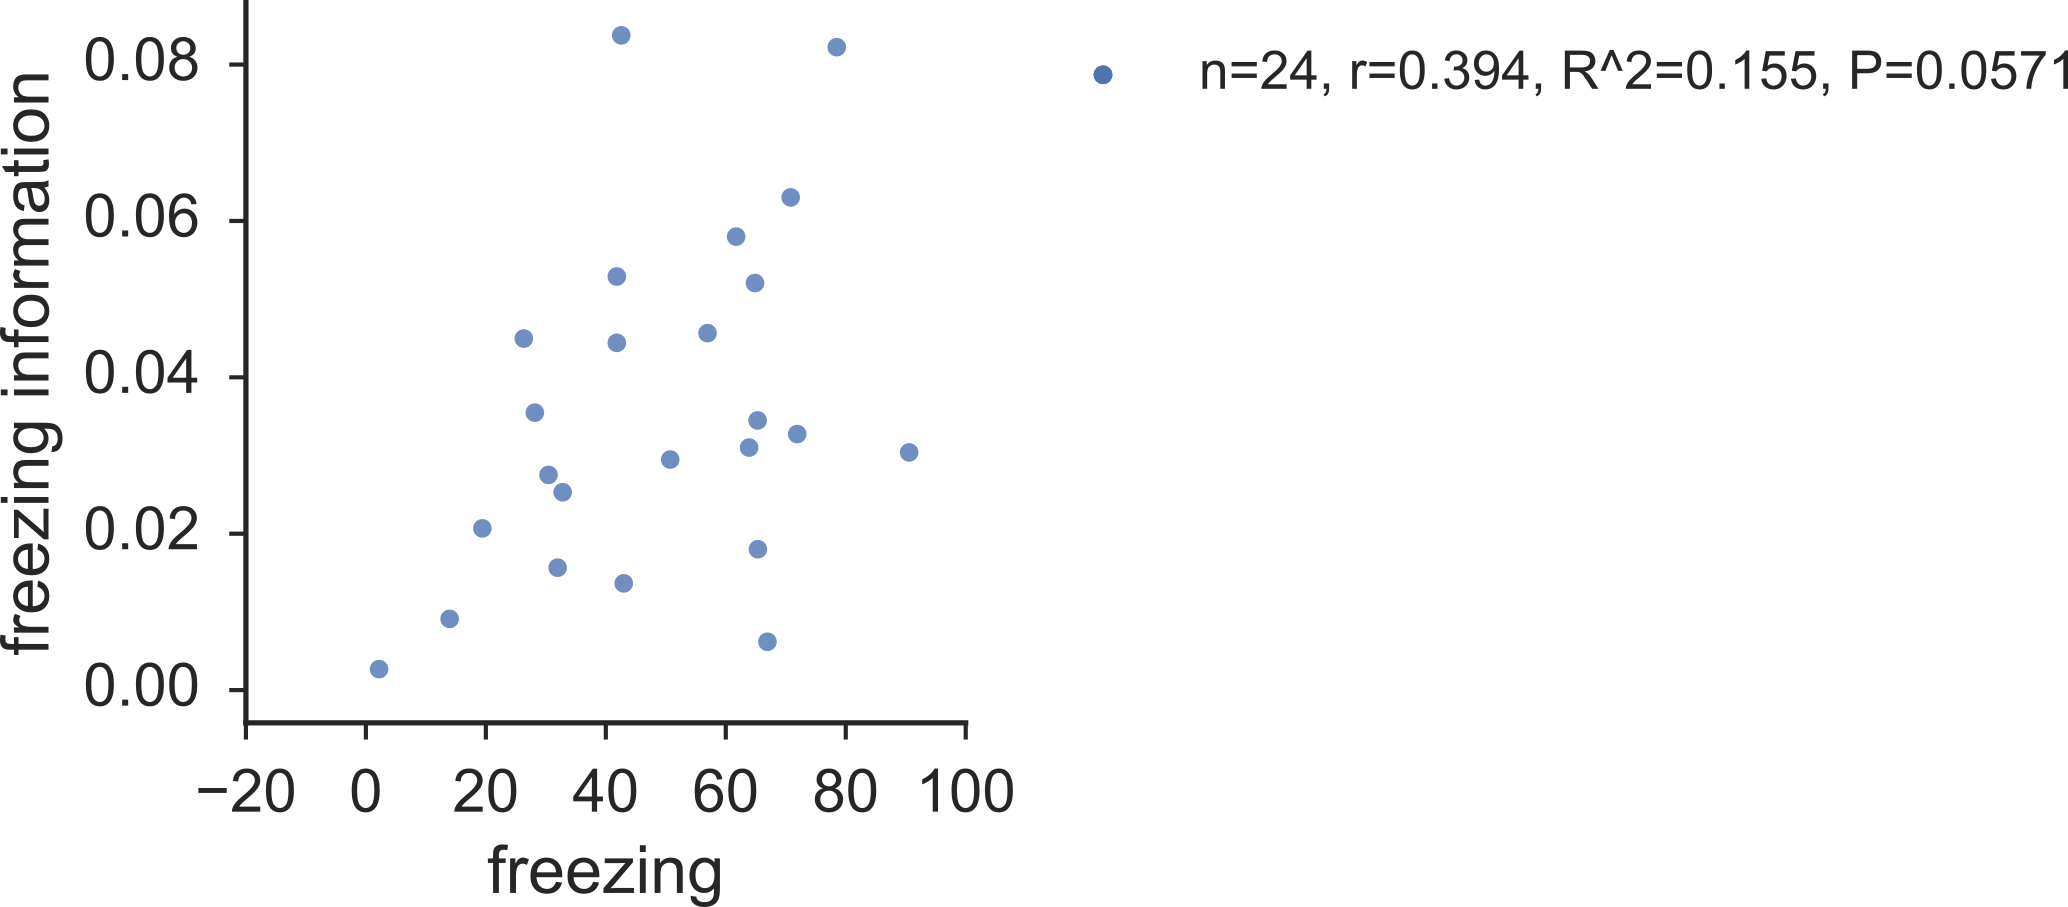
\includegraphics[width=\textwidth]{corr1.png}
        \caption{}
    \end{subfigure}
    \begin{subfigure}[t]{.5\textwidth}
        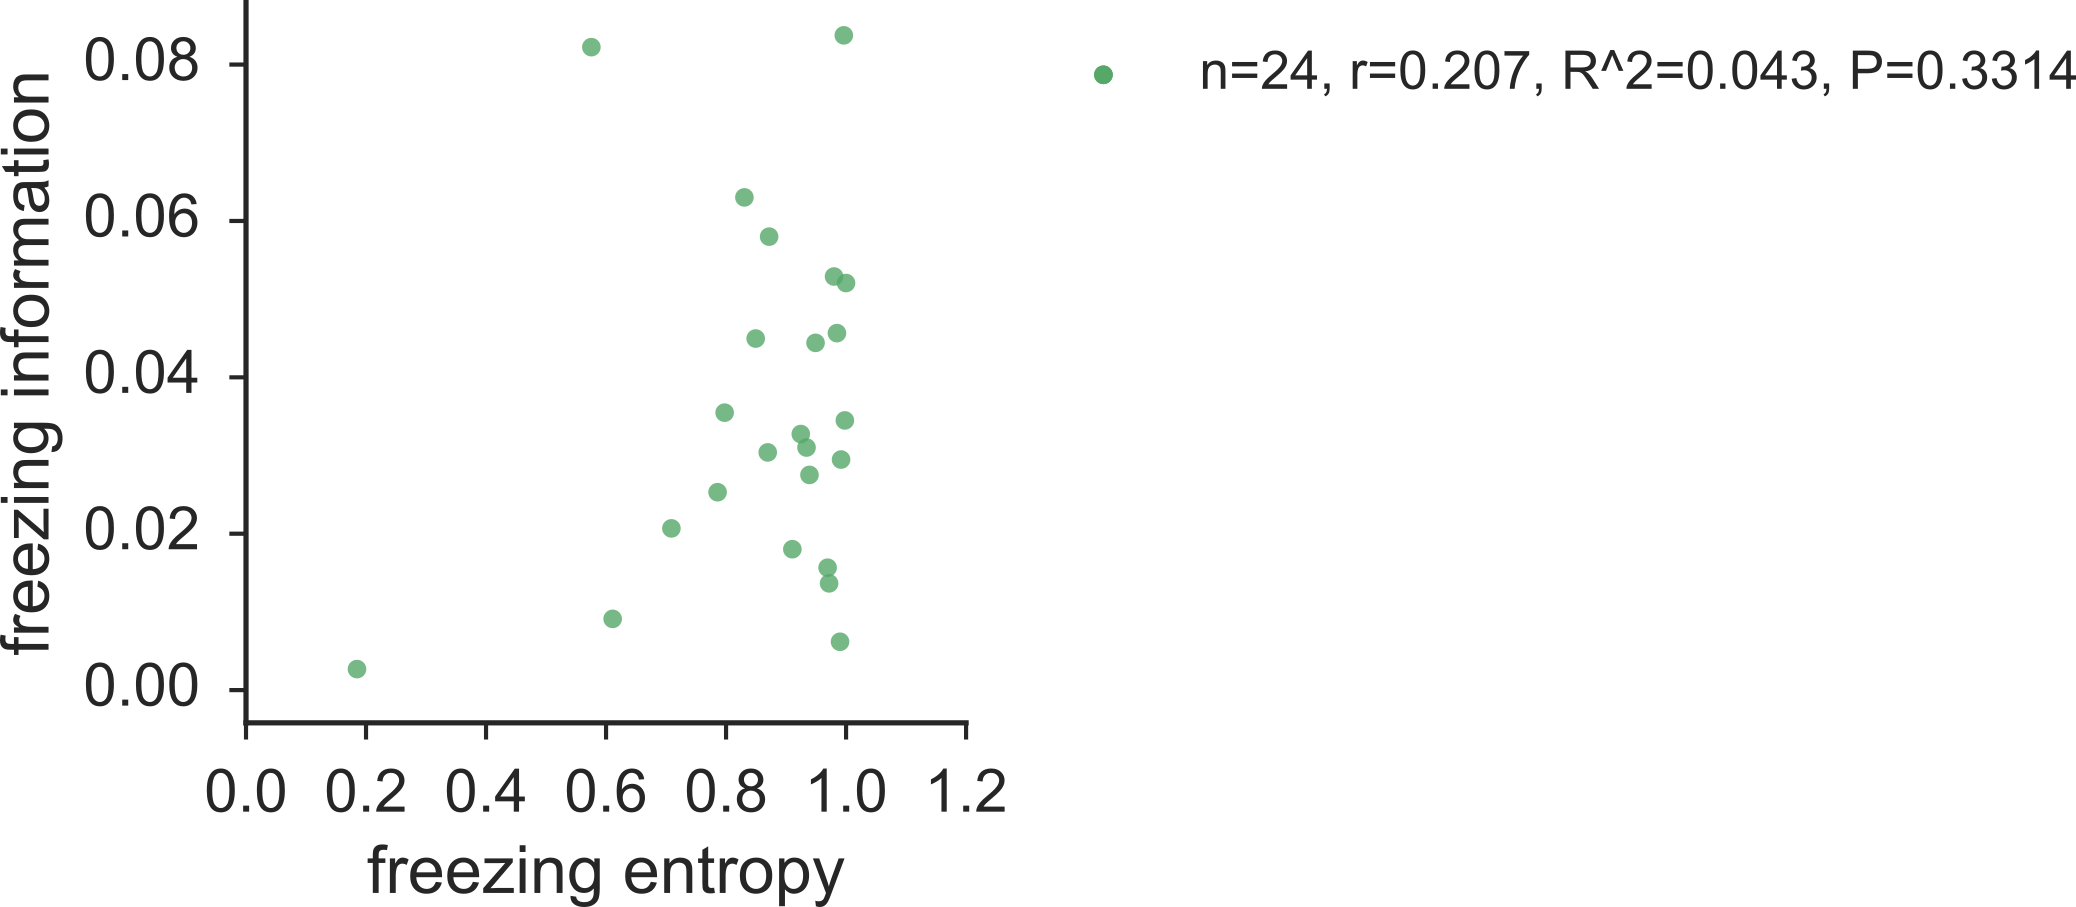
\includegraphics[width=\textwidth]{corr2.png}
        \caption{}
    \end{subfigure}
    \begin{subfigure}[t]{.5\textwidth}
        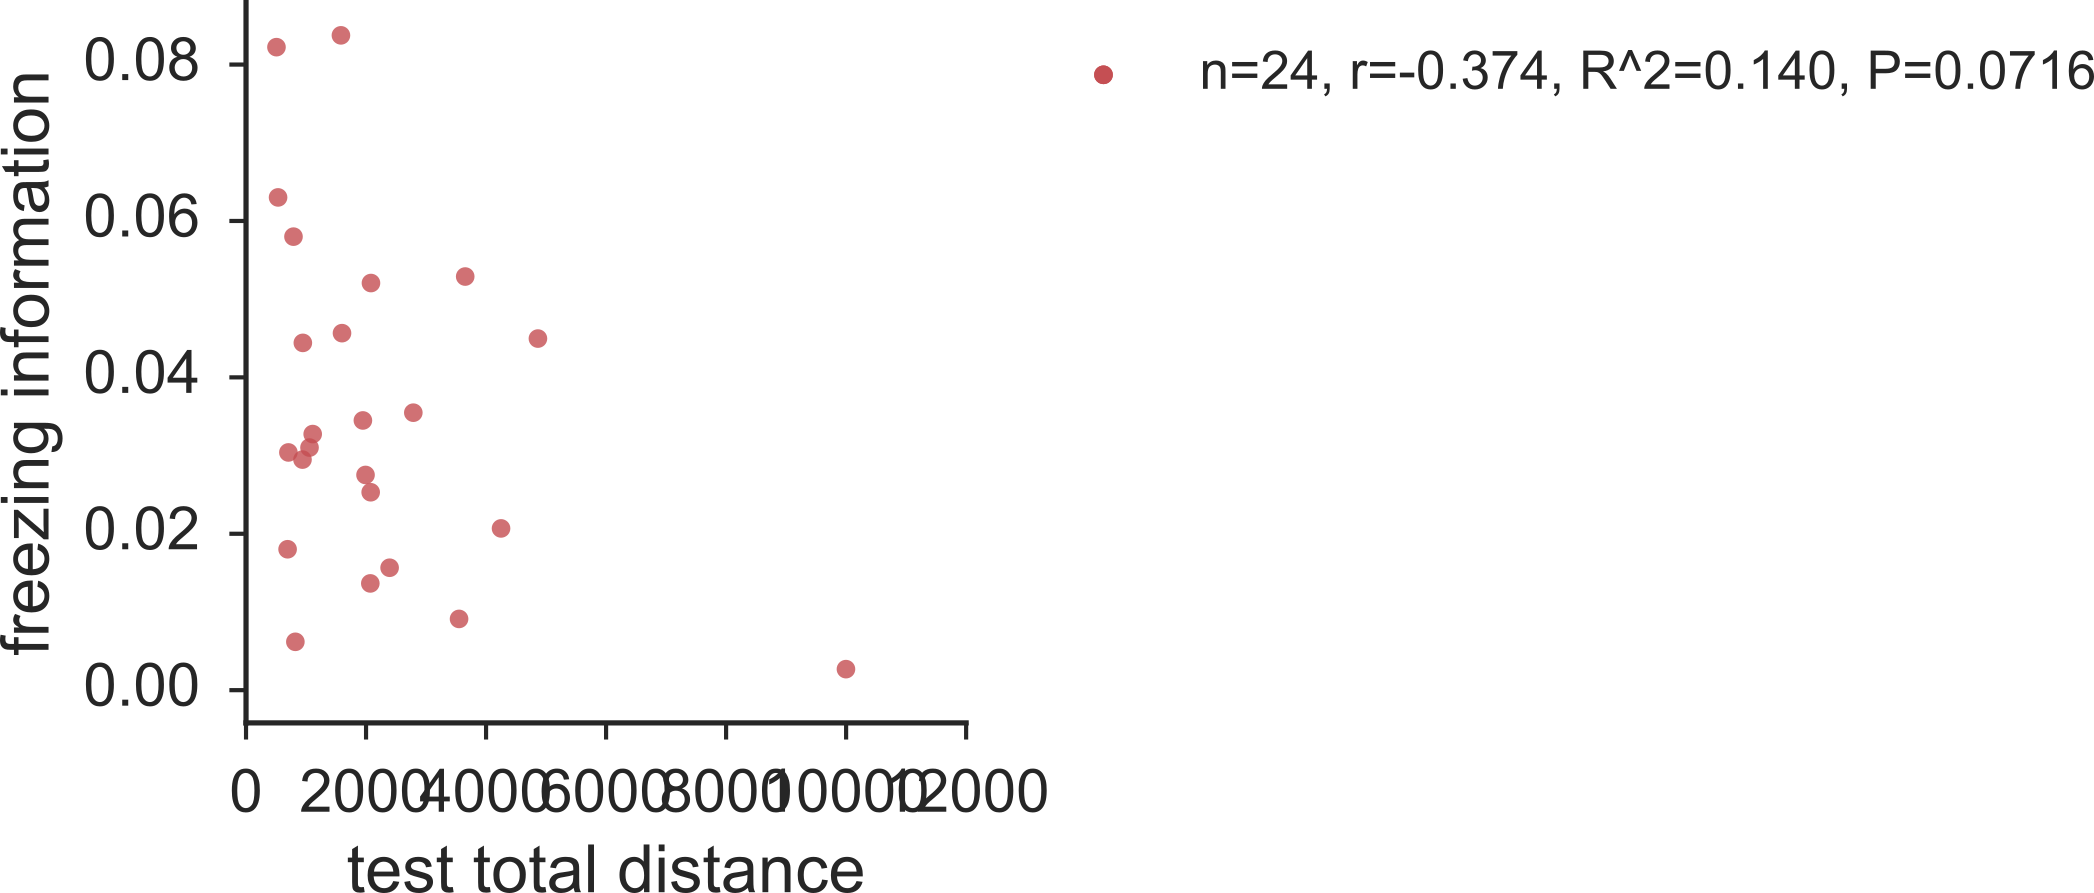
\includegraphics[width=\textwidth]{corr3.png}
        \caption{}
    \end{subfigure}
    \begin{subfigure}[t]{.5\textwidth}
        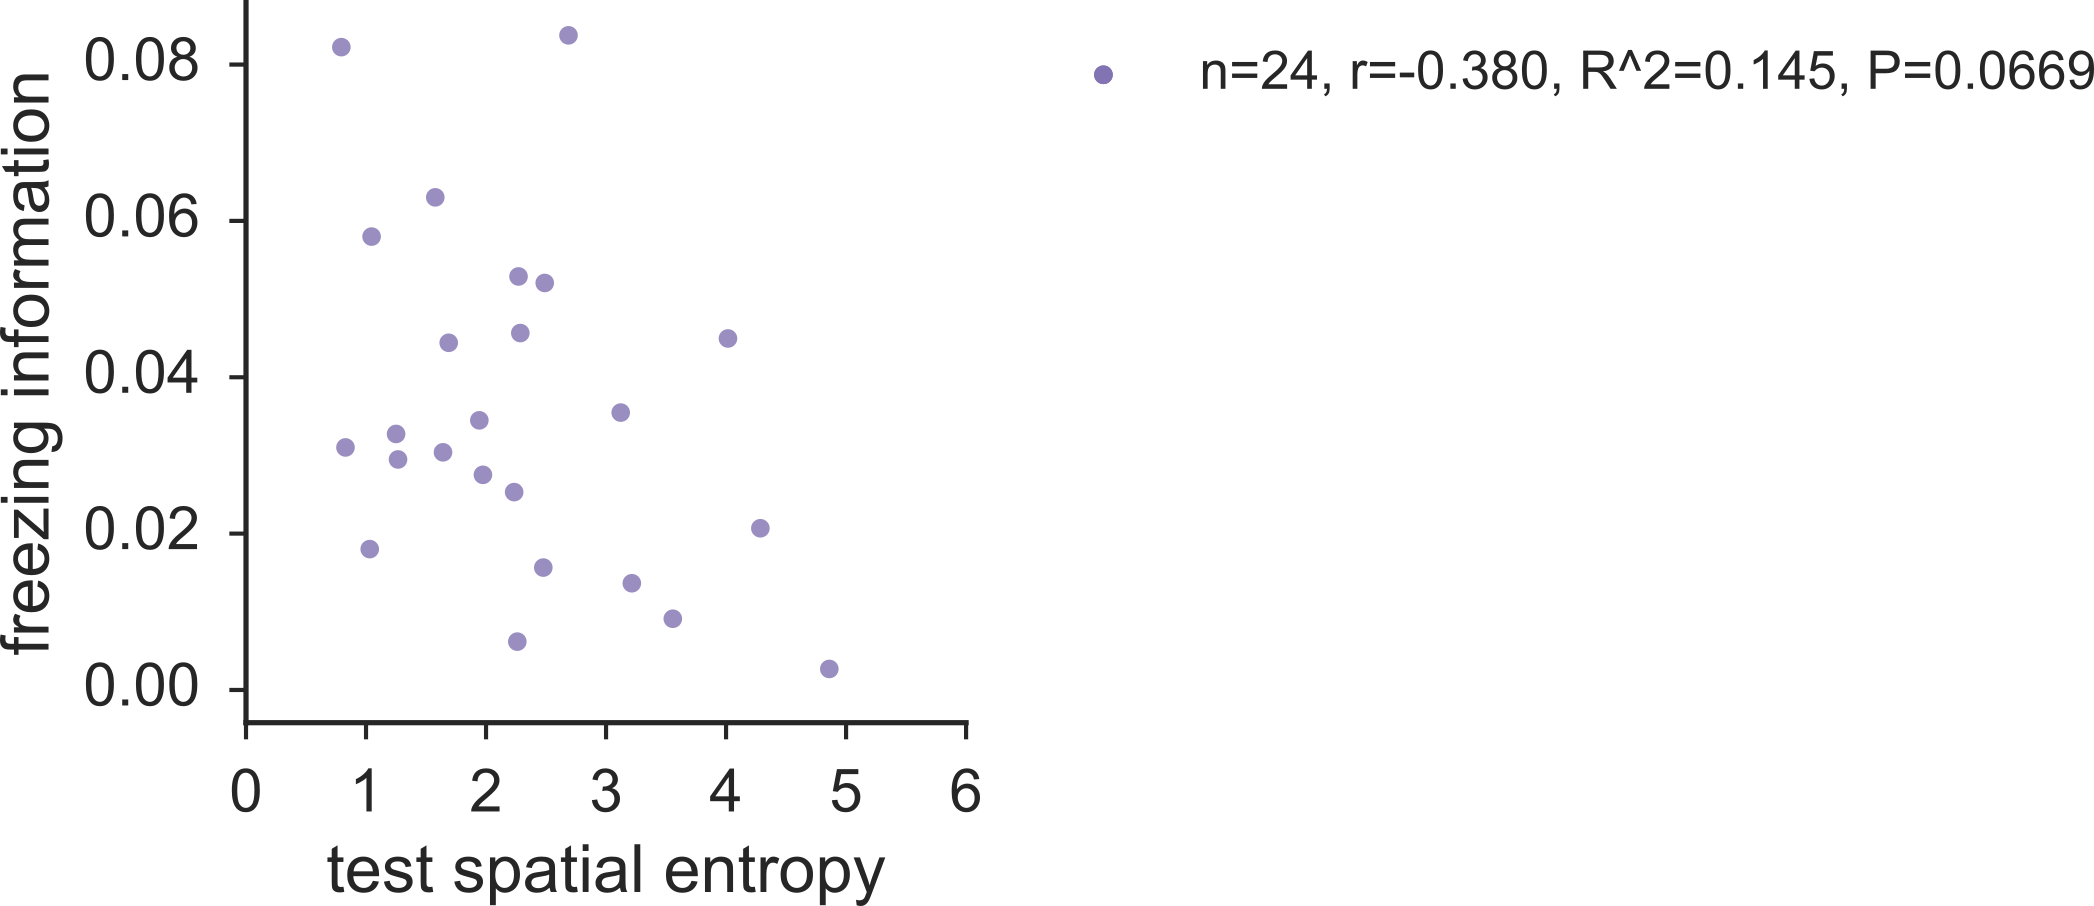
\includegraphics[width=\textwidth]{corr4.png}
        \caption{}
    \end{subfigure}
    \caption{Scatter plots of varies behaviour measurement against freezing information, in pooled \gls{wt}, \gls{wt}-\glu and \gls{tg}-\glu. Given there is no group difference between the three groups, if any of the behaviour factor is confounding, the it will contribute to within-group difference and correlate with freezing information. We have found no significant correlations. However the near significance of percent freezing and spatial entropy correlations will need further investigation. \label{f.ad.corrs}}
\end{figure}


\subsection{\tglu rescues recall by decreasing activity}

The next question we investigated is, if the cells are encoding freezing, how do they encode? In figure~\ref{f.ad.ch_activity} we selected all the cells that have more than 0.01 bits/second (which amounts to ~40\% in the normal groups and 10\% of the cells in the Tg group), and plotted the difference of average activity when the animal is freezing and not freezing. Interestingly, most of the cells encode freezing by decreasing their activity. This can also be seen representatively in the sample trace (Figure~\ref{f.ad.sample_trace}).
\begin{figure}[h]
    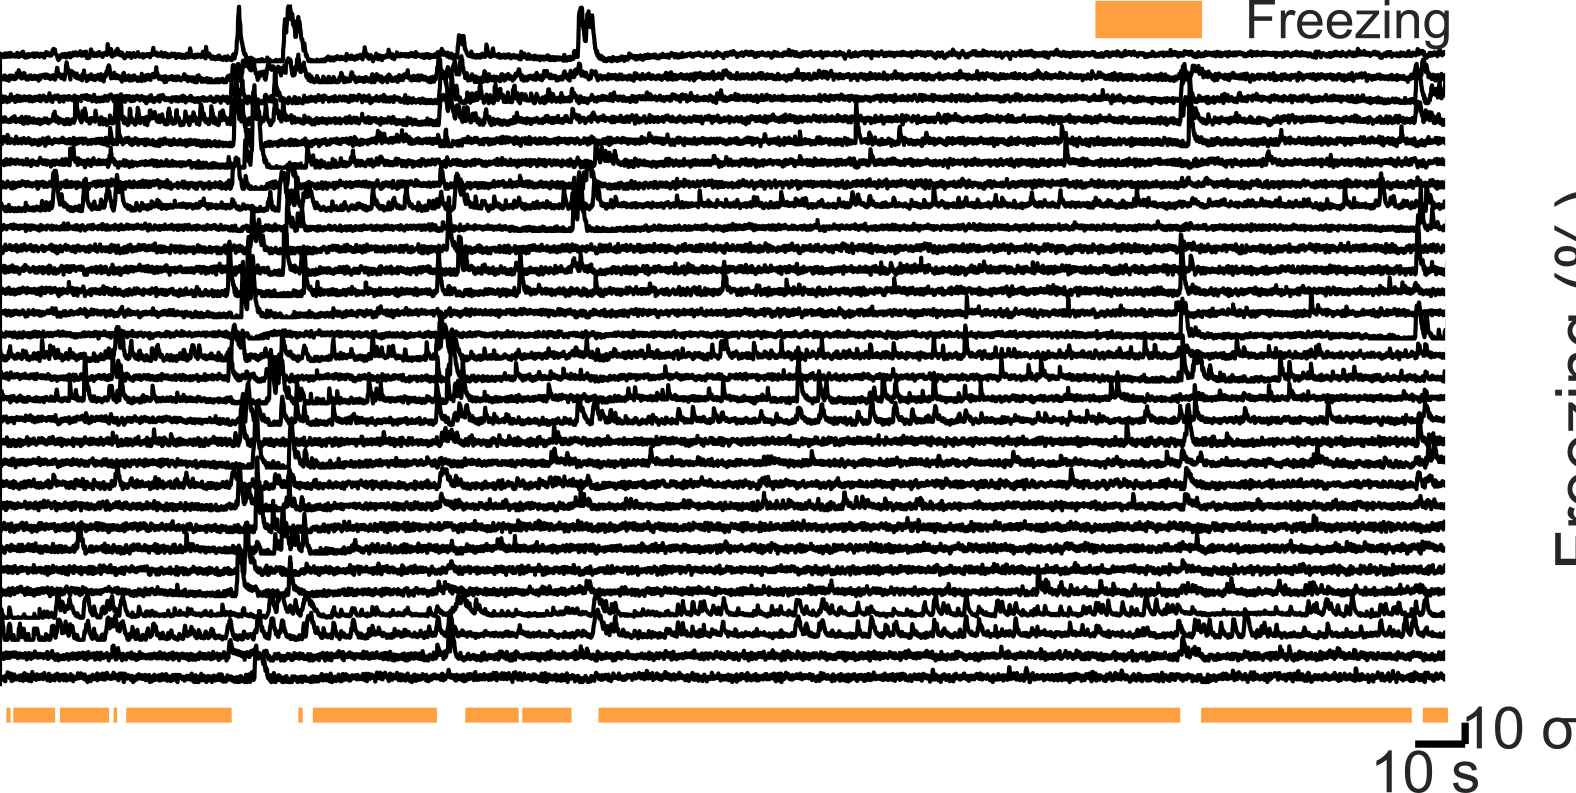
\includegraphics[width=\textwidth]{sample_trace.png}
    \caption{Sample traces from cells with highest freezing information in an animal. It appears that cells encode freezing by decreasing their activity. \label{f.ad.sample_trace}}
\end{figure}
\begin{figure}[h]
    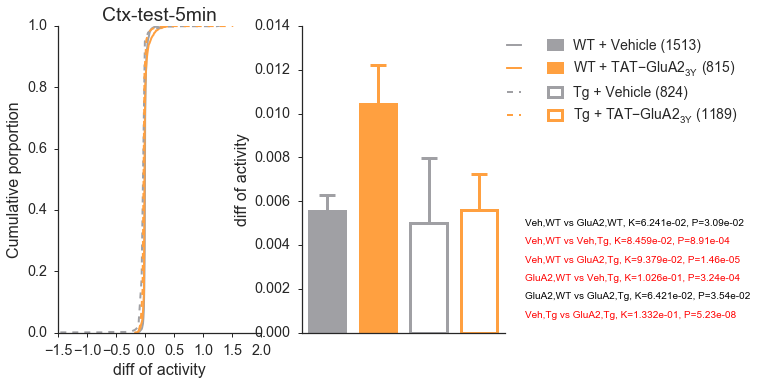
\includegraphics[width=\textwidth]{ch_activity.png}
    \caption{Distribution and mean of activity difference between freezing and none-freezing, in cell with freezing information more than 0.01. This confirms the intuition from Figure~\ref{f.ad.sample_trace} that most of the cells encode freezing by decreasing activity. \label{f.ad.ch_activity}}
\end{figure}

Given the cells tend to have decreased activity during freezing, we also examined the average cell activity when the animal is freezing, and activity when the animal is not (Figure~\ref{f.ad.activity_freezing}). Consistent with the freezing information result, the Tg animals have higher activity when the animal is freezing, and this is rescued by the \tglu. Interestingly, the rescue group also shows significantly decreased activity when the animal is not freezing. These results suggest the \tglu{} may rescue the Tg phenotype by globally decrease background cell activity.
\begin{figure}[h]
    \begin{subfigure}[h]{\textwidth}
        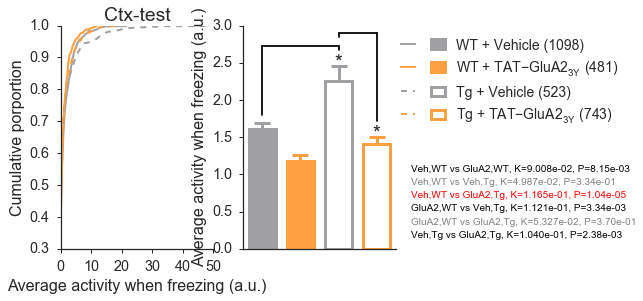
\includegraphics[width=\textwidth]{activity_freezing.png}
        \caption{\label{f.ad.actf}}
    \end{subfigure}
    \begin{subfigure}[h]{\textwidth}
        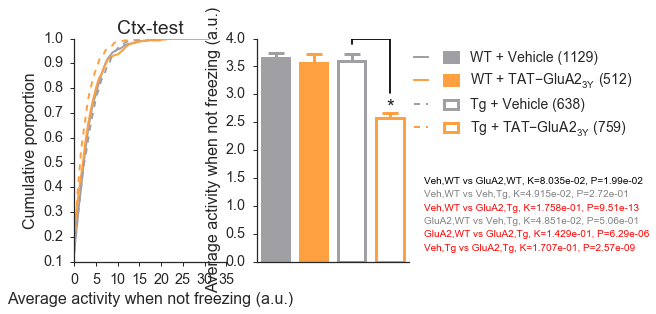
\includegraphics[width=\textwidth]{activity_moving.png}
        \caption{\label{f.ad.actnf}}
    \end{subfigure}
    \caption{Average cell activity during \subref{f.ad.actf} freezing and \subref{f.ad.actnf} not freezing. Cells in \gls{tg} animals have significantly higher activity during freezing, suggesting a sub-optimal encoding of freezing. Interestingly, \tglu also showed a decreased activity when the animal is not freezing, suggesting that the effect of \tglu maybe a global decrease of cell activity. \label{f.ad.activity_freezing}}
\end{figure}



\subsection{\Gls{tg} animals can initiate freezing}



\subsection{\Gls{tg} animals have deficits recall freezing memory}
\begin{figure}[h]
    \begin{subfigure}[h]{\textwidth}
        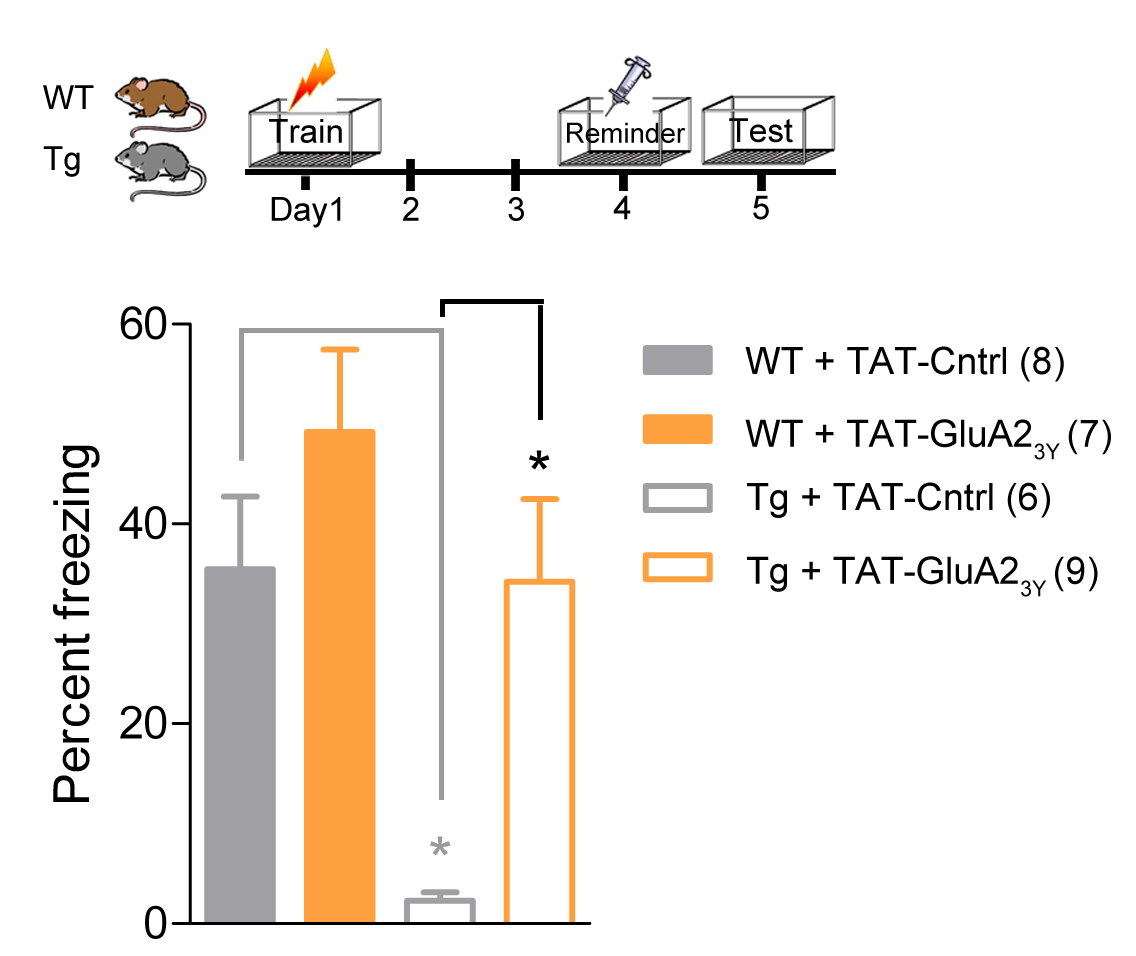
\includegraphics[width=\textwidth]{reminder1.png}
        \caption{\label{f.ad.actf}}
    \end{subfigure}
    \caption{ \label{f.ad.reminder1}}
\end{figure}

\section{Discussion}
\todo{Summary of result}
\todo{Hyperactivity}
\todo{Freezing encoding: not behavioural}
\todo{Direction of causation}
\todo{\tglu rescue - how?}

\chapter{General Discussion}
\section{Construction of the mini-microscope}
\subsection{Advantages of the current mini-microscope}
In the current project, we have constructed a miniature microscope which weighs less than \SI{3}{\gram}. The light weight of the mini-microscope allows for its implantation on mice without causing significant alterations to natural behaviour.  This miniature microscope is able to image green fluorescence at a resolution of at less \SI{2}{\um}. Using a tail vein injection of the fluorescent dye dextran-fluorescein, we are able to resolve individual red blood cells in capillary blood vessels, and measure the flow rate of the blood in the capillaries. 

Moreover, we have shown that the mini-microscope is able to record calcium transients from GCaMP-expressing neurons. Using the mini-microscope, we are able to image more than \num{200} \gls{ca1} neurons simultaneously, and identify potential place cells from the recording. Furthermore, with the addition of a thin relay \gls{grin} lens, we are able to extend the imaging capability of the mini-microscope to deep brain regions with minimal damage to the tissue. Here we have demonstrated simultaneous recording of more than \num{40} neurons in \gls{la} while an animal undergoes auditory fear conditioning. 

In this project, we recorded calcium transients at a rate of \num{20} frames per second, but this does not represent a limit in the frame rate. With the XIMEA camera (MU9PM), the recoding rate can reach up to \num{200} frames per second at a cost of exposure and spatial resolution. A higher frame rate will allow identification of fast brain oscillations such as the \SIrange{7}{11}{\hertz} theta oscillation and potentially the fast \SIrange{40}{100}{\hertz} gamma oscillation, both of which have been shown to be important in learning and memory. Calcium imaging is especially suited for detection of brain oscillations, as these oscillation may not lead to action potentials, but create sub-threshold changes of membrane potential which would be reflected by a fluctuation of internal calcium concentrations. The ability to simultaneously image a dense ensemble of neurons allows brain oscillations to be measured in each cell, and the \gls{snr} in detecting these oscillations can be increased by averaging signals from all cells and even background fluorescence. The brain oscillation signal can then be related to neural activities to study how local neural circuits respond to the brain oscillation. 

In the current project, we have also demonstrated the ability of the mini-microscope to image in both red and green channels. The extra colour channel can be used for the identification of neural subpopulations or for gathering extra information from the brain. In our prototype we used blue light to stimulate red retrobeads and the fluorescent protein tdTomato, both of which have a broad excitation spectrum. However, this requirement is usually not necessary. If the red channel is static, it can be captured by a separate mini-microscope with an efficient excitation \gls{led} and corresponding filters just for the red fluorophore. The resulting image can be later aligned with recording of calcium transients for cell identification. 

Our design of mini-microscope costs \$\,300--\$\,1000 for each unit, which will not represent a significant expense in most neuroscience laboratories. Moreover, all components of the mini-microscope are commercially available and can be assembled with minimal tools, providing access to neuroscientists with no requirement of engineering experience. The microscope casing is 3D printable. We will make both the 3D models and relevant analysis code freely available in order to open this work to the neuroscience community.

\subsection{Advantages of using the mini-microscope to study \gls{ad}}

As a test of the usefulness of the miniature microscope, we used it to image \gls{ca1} neurons in a transgenic mouse model of \gls{ad}, TgCRND8, while the mice encoded and recalled a contextual fear memory. On average, we were able to image more than \num{100} neurons simultaneously for each mouse, and this data enabled us to investigate hippocampal circuitry mechanisms in \gls{ad}.

The importance of the mini-microscope in understanding neural circuitry mechanisms is particularly reflected in the classifier prediction results. We have found that the \gls{nbc}, which predicts mouse behaviour by considering individual neurons, is unable to reveal the pattern completion deficit in TgCRND8 mice. This result suggests that a significant amount of information the neurons are encoding is contained in the synergy between activity of neurons. This information cannot be revealed using traditional methods such as \textit{in vivo} electrophysiological recording, where only a handful neurons can be recorded at the same time. To compensate for the scarcity of simultaneously recorded neurons, electrophysiological recordings often require experimenters to repeat the same behaviour trial many times, which may lead to changes in the animal's behaviour and a potential confound in the interpretation of the data. However in the current study, the mini-microscope has given us the freedom to choose an experimental paradigm which is well-established in the field of behavioural neuroscience. This freedom allowed us to connect the findings from the neural activity recordings to the rich findings of behavioural neuroscience. This stands in contrast to \textit{in vivo} 2-photon imaging, where due to the requirement of head fixation, only specifically designed behavioural paradigms are compatible, whose neural mechanisms are less well understood. 


\section{Examining circuitry deficits in a mouse model of \gls{ad}}

\subsection{\gls{ca1} hyperexcitability}
We found that in TgCRND8 mice, \gls{ca1} neurons are more active than those in \gls{wt} mice, both during context exposure and during contextual memory recall. \tglu{} treatment during training is able to reduce the overall cell activity to \gls{wt} level. Moreover, to control for the behavioural state of the mice, we investigated cell activity when the mice were both freezing and active. We found the TgCRND8 genotype has a significant effect on increasing cell activity during freezing, and \tglu{} treatment reduces cell activity in both \gls{wt} and TgCRND8 mice. When mice were not freezing during the memory test, only TgCRND8 mice treated with \tglu{} has a significant decrease in cell activity compared to the other three groups. 

Our results confirm previous findings that \gls{ca1} cells in \gls{ad} are hyperactive \citep{palop16}. We have also found that while during memory test, the average cell activity in \gls{wt} mice is at the same level as it is during contextual exposure, cell activity in the TgCRND8 mice increases during memory testing compared to the memory encoding session (Figure~\ref{f.ad.actdiff}). This result suggests that in addition to the hyperactivity introduced by \gls{ad} pathology, the TgCRND8 mice show additional activity in response to the memory recall task. This finding parallels evidence from human patients with early \gls{ad}, where \gls{fmri} studies have found hyperactivity in the hippocampus only during memory recall, and that this negatively correlates with memory performance \citep{sperling09, reiman12, kunz15}. It has been hypothesized that this task-dependent increase of hippocampal cell activity may be a compensatory mechanism in response of degraded hippocampal function in \gls{ad} \citep{kunz15}.

While hyperexcitability in \gls{ad} mice is present when the mouse is freezing, cell activity when the mouse is not freezing does not differ between groups. Considering that the majority of \gls{ca1} cells lower their activity during freezing, it is possible that the hyperactivity of \gls{ca1} neurons is caused by an inability to keep silent. This is congruent with the \gls{nmdar} pathology seen in \gls{ad}, where \glspl{nmdar} are found to spontaneously activate in \gls{ad}, and cause excitation in the neuron \citep{danysz12}. This result is also hinted at by \citet{cheng13}, who investigated spatial encoding in another mouse model of \gls{ad}. In their study, when a mouse was in the receptive field of a place cell, the cell was normally active. However when the mouse was outside the receptive field of the place cell, the cell was unable to stop firing, leading to enlarged place fields \citep{cheng13}. 

It is somewhat counter-intuitive that the \tglu{} treatment, which increases synaptic \gls{ampar} density and therefore strengthens excitatory synapses, results in a decrease of overall neural activity in \gls{ca1}. However, considering that the hyperexcitability in \gls{ad} is hypothesized to be the result of increased \gls{ltd} and decreased \gls{ltp} in the synapse (discussed in Section~\ref{ad.synaptic}), and \tglu{} has been shown to block \gls{ltd}, it is possible that \tglu{} treatment rescues excitability by reversing the \gls{ltp}--\gls{ltd} imbalance. It is still unclear how an \gls{ltp}--\gls{ltd} imbalance leads to hyperexcitability. Computational models of \gls{ad} neurons suggest this may be caused by a loss of synaptic spines in hippocampal neurons. This morphological change of neuronal dendrites in \gls{ad} creates less hindrance for the transmission of incoming \glspl{epsp}, therefore allowing the neurons to be more excitable \citep{siskova14}. It is possible that \tglu{} rescues hyperexcitability by restoring the morphology of the neurons. There is a close correlation between synaptic \gls{ampar} density and spine size, and endocytosis of GluA2-containing \glspl{ampar} can trigger changes in dendritic spine size \citep{hanley08}. Indeed, in unpublished data from this project, we have found \tglu{} treatment protects from spine density decreases in both \gls{ca1} and \gls{dg} after an acute expression of \gls{app}, supporting the possibility that \tglu{} rescues hyperexcitability by restoring normal neuronal morphology in \gls{ad}. 

The \tglu{} treatment was applied to TgCRND8 mice only \SI{1}{\hour} before contextual fear training, however the effect of \tglu{} was present both during contextual fear training and during memory testing. This suggests that \tglu{} starts to affect cell excitability within \SI{1}{\hour}, and has long-term effects. A closer investigation of cell activity during training shows that, while \tglu{} is able to correct average cell activity in TgCRND8 mice to \gls{wt} level, the distribution of cell activity between Tg-\tglu{} and WT-Veh is still significantly different. From the cumulative plot (Figure~\ref{f.ad.acttrain}), the distribution of the lower \SI{90}{\percent} of cell activity in Tg-\tglu{} is similar to WT-Veh, however activity of the most active \SI{10}{\percent} of cells are similar to Tg-Veh. This difference is not present \SI{24}{\hour} later during memory testing. This suggests that the rescuing effect of \tglu{} is a gradual process which take hours to complete. Cells that are less hyperactive are first rescued, and cells with very high activity require longer time for the effect of \tglu{} to appear. Given that cells close to amyloid plaques are more excitable \citep{busche12}, it is possible these cells with very high activity are located near amyloid plaques, have more damage from the \gls{ad} pathology, and require longer time for the pathological process to reverse. 


\subsection{Contextual fear memory}

In this project, we subjected \gls{wt} and TgCRND8 mice to contextual fear conditioning, and found that while the TgCRND8 mice show inferior memory during testing, this memory deficit can be rescued by \tglu{} treatment either during training, or during exposure to a brief reminder. This result suggests that TgCRND8 mice are still able to encode the memory during training, however have deficits in recalling the memory during testing. Similar results have been reported previously. In another mouse model of early \gls{ad}, APP/PS1, \citet{roy16} tagged cells activated during contextual fear conditioning, and optically activated these cells during memory recall. They found that while the APP/PS1 mice showed a memory deficit during memory recall, light stimulation of the contextual fear memory trace was able to induce memory expression. 

In order to distinguish whether the memory recall deficit is due to initiation or maintenance of memory expression, we have also analyzed the number of freezing bouts and duration of freezing bouts in TgCRND8 and \gls{wt} mice. We found that while the TgCRND8 mice do not show a significant difference in number of freezing bouts during memory test, the duration of these freezing bouts are significantly shorter than those of the \gls{wt} mice. This result suggests that the TgCRND8 mice are still able initiate the memory recall, however are unable to maintain it. 

\subsection{Encoding}

In the current study, we have found that cell activity in TgCRND8 mice is not as predictive of fear memory expression as that in \gls{wt} mice. On the other hand, this deficit is not reflected in the prediction accuracy of the machine learning classifiers: both \gls{nbc} and \gls{gsvm} are able to predict freezing from cell activity in TgCRND8 mice as well as in \gls{wt} mice. This discrepancy of the prediction power suggests that the hippocampal neural circuit is highly redundant, such that even when the prediction power of individual neurons is negatively affected by \gls{ad}, there is no significant information loss if multiple neurons are combined to make a prediction. Similar results are found in place encoding, where while individual neurons in a \gls{ad} mouse model have degraded spatial encoding \citep{cacucci08,cheng13,mably17}, the ensemble is still able to accurately represent the mouse's position \citep{cheng13}.  

In this study, we only recorded close to one hundred cells in \gls{ca1} for each mouse on average, and the information in the activity of these neurons is enough for an accurate prediction of the mouse's fear memory recall. There are more than \num{1e4} neurons in \gls{ca1}: therefore even if under \gls{ad} pathology where individual cells' firing patterns are degraded, any downstream brain structure should still able to decode the information. This then suggests that the degradation of individual cell activity in \gls{ad} is secondary to the cognitive deficit, since to an efficient downstream brain structure, redundancy in the brain can protect information loss due to the degradation of cell activity. 

This conclusion also explains why in the preclinical population, significant \gls{ad} pathology often does not impact cognitive performance (Discussed in Section~\ref{preclinical}). Another important implication of this conclusion is that treatment of the \gls{ad} pathology alone, without any restoration of the neural network structure, will not result in a significant improvement in cognitive symptoms. This may explain the failure of recent attempts at treating \gls{ad} with \abeta{} clearance: it is possible that even with the successful \abeta{} removal, additional intervention is still required to restore the neural network at a circuitry level.

The importance of neural network structure is also reflected in the difference of \gls{gsvm} and \gls{nbc} performance. The significantly improved performance of the \gls{gsvm} suggests that the network encodes more information than individual cells. This may be a universal phenomenon across the brain, as it has also recently been found in other brain regions such as \gls{bla} during auditory fear conditioning \citep{grewe17}. Moreover, we find the accuracy of the \gls{gsvm}, which predicts freezing based on the cell assemble as whole, is again similar to \gls{wt} mice. This suggest that when a mouse is freezing, the information contained in the activity of the neural network in \gls{ad} mice is unaffected. 

\subsection{Pattern completion}

Given that the neural network contains can accurately predict freezing in \gls{ad} mice, it is intriguing how the AD mice have a memory deficit at all. During memory expression, the information content for the cell ensemble in \gls{ad} is not different from that of the \gls{wt} mice, and it is therefore possible the memory deficit can be detected outside of the duration where the memory is expressed. Given that the memory deficit in \gls{ad} is a deficit in memory recall, and that the process of pattern completion in hippocampus is theorized to be important in memory recall, we investigated whether this process is affected in the TgCRND8 mice.

To detect the pattern completion process, we aligned classifier prediction accuracy to the time point when the mice show behavioural change (Figure~\ref{f.ad.into_f}). We found a significant drop of prediction accuracy just prior to freezing, both in the \gls{nbc} and \gls{gsvm}. Since the drop in accuracy happens at a time where mice are predominantly not freezing, the accuracy drop suggests that the classifiers are (inaccurately) predicting freezing, before mice start to freeze. 

Since the classifiers are trained on each time point shuffled, they are agnostic to the temporal dynamics of cell activity. Therefore, the significant change of prediction accuracy before freezing must reflect changes in the pattern of neural activity itself. Moreover, the fact that the change of neural activity in \gls{ca1} is present before behaviour onset is very important in interpreting findings of the this study. Given that nature of the study is correlational, the causal relationship between neural activity and behaviour is unclear. However, the temporal precedence of \gls{ca1} activity suggests that the neural activity pattern is not a result of the mouse's behaviour,  but likely involved in initiating the behaviour. This confirms that the neural activity difference we have found between treatment and genotype groups is a result of circuitry deficit, instead of a consequence of different behaviour between mice. 

We have found in \gls{nbc} prediction, the temporal signature of freezing behaviour in \gls{wt} mice precedes the other three groups. Given that the \gls{nbc} considers each cell individually, this result suggests that the activity of individual cells start to form a ``cellular signal'' for freezing, which is a measurement of the contextual fear memory recall. The findings that all groups in \gls{nbc} predict freezing before behaviour, and that they have similar temporal precedence over behaviour suggest that in \gls{tg} mice, the ``cellular signal'' for contextual fear memory recall is unaffected. 

On the other hand, we found that the \gls{gsvm} prediction precedes freezing in \gls{wt} mice, however this is not present in the vehicle-treated \gls{ad} mice. Again, given that the \gls{gsvm} detects a network pattern of cell activity, this result suggests that in \gls{wt} mice, a ``network signal'' of freezing appears in the \gls{ca1} network, however this signal is missing from the \gls{ad} mice before freezing. 

As the \gls{gsvm} can accurate classify the behavioural state of mice based on their neural activity, we can use the \gls{gsvm} to approximate the neural activity pattern of recalling a contextual fear memory (considering each freezing bout as an episode of memory recall). The gradual rise of freezing prediction before the freezing behaviour therefore represents the process of pattern completion: where an incomplete freezing pattern first appears in the network and confuses the classifier's attempt to predict freezing. Over time, the pattern gets more complete, which leads to increased classifier prediction of freezing. 

\begin{comment}
It is worth noting that while computational studies often model pattern completion using a stationary pattern \citep{rolls13}, our data suggest that the neural correlate of the contextual fear memory recall cannot be explained by a stationary attractor state. In a stationary attractor state, 

The prediction accuracy of the \gls{nbc} and \gls{gsvm}

the difference in prediction accuracy between \gls{nbc} and \gls{gsvm}, as well as the different temporal dynamics of the prediction precedence suggest that the neural correlates of a contextual fear memory recall is not a stationary state, since otherwise the performance of \gls{nbc} and \gls{gsvm} should be very similar, and have similar temporal dynamics in pattern completion. \todo{This is a pretty long sentence!  You should try and break it up} Therefore, our result suggests that even in an apparently ``simple'' memory such as the contextual fear memory, the neural correlates are dynamic: the state of neural activity during memory recall can move between multiple states.
\end{comment}

We found that the ``cellular signal'', as detected by the \gls{nbc}, appears significantly earlier than the ``network signal'' from the \gls{gsvm}. This result reveals some details about the pattern completion process. The pattern completion process starts with individual cells changing their firing rate to that representing their activity distribution during memory expression, potentially guided by feed-forward input. However, as the memory pattern is a collection of patterns, at any single point each cell may have the activity from different patterns. Therefore at this time point, \gls{nbc}, which only classifies by examining whether the activity of individual neurons represents \textit{any} single contextual fear memory pattern, is able to detect a pattern for fear memory recall. However as the cell activities are not synchronized, no significant global pattern can be detected by \gls{gsvm}. 

However, as the ``cellular signal'' grows stronger, some cell activities become synchronized, and form a partial global pattern. This global pattern then, potentially through recurrent connections, recruits more cells to join the pattern. At this time, the partial global pattern can be detected by the \gls{gsvm}, and this positive feedback loop continues until the pattern is complete. This pattern then forms an attractor of brain states, which maintains itself despite small fluctuation in the feed-forward input, and only disappears when there is a large shift of the feed-forward input which significantly deviates the neural activity pattern from the contextual memory pattern \citep{rolls13}. 

It is easy to fit the specific deficit of \gls{ad} mice within this interpretation. \gls{ad} mice show normal dynamic of ``cellular signal'', however they are missing the ``network signal''. It is therefore possible that the \gls{ad} mice have a deficit in pattern completion: that the positive feedback force of converting an asynchronous ``cellular signal'' to a ``network signal'' is degraded. The lack of a gradual network signal suggest that the ``network signal'' in the \gls{ad} mice is likely formed by chance, that at some point, a global pattern appears from the asynchronous activity of individual cells. 

%This interpretation has several predictions. First, it predicts that the synchronization of cell activity in the \gls{ad} mice is degraded. To test this hypothesis, we calculated correlation of the neural activity of each pair of neurons, and compared the distribution between \gls{wt} and \gls{tg} mice. And indeed, we have found that cells in the \gls{tg} mice have less correlation with each other \todo{ref correlation figure}. 

This result is also supported by reports of neural oscillation deficits in \gls{ad}. In hippocampus, the \SIrange{3}{12}{\hertz} theta oscillation and the faster \SIrange{25}{120}{\hertz} gamma oscillation are considered important for learning and memory, and are critically dependent on the integrity of hippocampal neural networks \citep{buzsaki02, colgin09}. However, both theta and gamma oscillation has been shown to be altered in rodent models of \gls{ad}. It has been reported that the progression of plaque deposition is correlated with a decrease of theta power and frequency in both mouse models of \gls{ad},and acute \abeta{} treatment in rat \citep{scott12, villette10}. Decreased oscillation power is also found in the gamma frequency, and removal of \abeta{} plaques is able to block the deficit \citep{driver07, kurudenkandy14}. The coupling of theta and gamma oscillations has also been reported to be affected in \gls{ad} \citep{goutagny13}. 

Similar oscillation deficits are also found in the human patients. \Gls{eeg} recordings in early \gls{ad} patients have shown a decreased coupling between parietal alpha and prefrontal theta oscillations, and event-related delta, theta and alpha coherences are also significantly decreased \citep{guntekin08, montez09}. Moreover, the prefrontal theta coherence increases in \gls{ad} patients treated with \gls{ache} inhibitors \citep{yener07}, suggesting a close relationship between brain oscillations and \gls{ad}. More recent studies have aimed to enhance brain oscillations in \gls{ad}, and have suggested a causal relationship between the two. It has been found that deep brain stimulation at gamma frequency, both in rodent models and \gls{ad} patients, is able to improve cognitive function \citep{suthana14}. A recent study also showed that in a mouse model of early \gls{ad}, induction of gamma oscillation also reverses \abeta{} deposition \citep{iaccarino16}. 

These results suggest that the pattern completion deficit in \gls{ad} may be closely related to the brain oscillation deficit reported in the literature. However in the current study the cell activity is recorded at \SI{20}{\hertz}. The sampling frequency is unfortunately too slow to allow detection of any brain oscillations above \SI{10}{\hertz}. How a deficit in brain oscillation affects the pattern completion process in \gls{ad} is an important topic for future research. 

Secondly, this interpretation suggests that \gls{ad} mice may still be able to initiate freezing, however due to degraded attractor functions, they are unable to maintain the state of memory recall. This is supported by our findings that the \gls{tg} mice have similar number of freezing bouts, however a significantly shortened bout duration, showing a deficit in maintaining the expression of the memory but not initiating the memory. 

Moreover, the instability of the memory state in \gls{ad} can be inferred from the distance to the boundary of memory states. We measured the signed distance to the \gls{gsvm} classification boundary when the mouse's behaviour transitioned into freezing (Figure~\ref{f.ad.cls-distance}). We have found that while \gls{wt} mice show an acceleration over and away from the boundary, the \gls{tg} mice only barely cross the boundary, and stay close to it during freezing. Therefore, a small perturbation in the brain state is more likely to shift the \gls{tg} mice out of freezing. The freezing state in the \gls{wt} mice, on the other hand, is more robust to small perturbations.  

While the current study is the first to suggest that neural attractor states for memory recall are unstable in \gls{ad}, evidence from human behavioural studies suggest that similar dynamics may exist in \gls{ad} patients for other cognitive functions. Attention has long been considered computationally as a result of neural attractor states, and the strength of the attractor is important for maintaining attention \citep{desimone95, rolls08a, rolls13a}. Interestingly, early \gls{ad} patients have no deficits in focusing the attention, however, their attention is more likely to be disrupted by distractors, and less likely to be maintained over time \citep{perry99}. This result is similar to the memory recall deficit we have found in the current study, suggesting that it is possible that the deficit in attractor state in early \gls{ad} is global, affecting many brain areas' cognitive functions. 

The fragility of the memory attractor in \gls{ad} may also implicate another curious deficit of \gls{ad} called subjective memory impairment \citep{jahn13}. Subjective memory impairment is defined as a sense of memory deterioration with no objective impairment in cognitive test. Subjective memory impairment is correlated with hyperactivation of the \gls{mtl} during memory tasks, and predictive of hippocampal atrophy as well as later development of cognitive impairment and \gls{ad} \citep{jahn13}. It is possible the subjective memory impairment arises from our finding that during memory recall, the network state in \gls{ad} tends to stay close to the boundary of the attractor state. This close distance can be detected by other brain regions, and reduce the confidence of those brain regions in predicting the patient's behaviour, creating a sense of unsureness without a degradation of performance.  

The deterioration of the attractor state in \gls{ad} can be caused by several factors. First, we have shown that the deficit in \gls{ad} mice can be rescued by \tglu{} treatment with a reminder. From this we conclude that the \gls{ad} mice have encoded the contextual fear memory during training, but that this memory may not be encoded in the same way as in \gls{wt} mice. Therefore, the attractor state deficit can be a result of the formation of a weak attractor for the memory. Given that the neurons in \gls{ad} have impaired \gls{ltp}, and the normal memory encoding process may be interfered with by hyperactive neurons, it is unlikely that the memory encoding process is completely spared. 

Secondly, it is also possible that interference exists during the memory recall. The hyperactivity observed in the \gls{ad} mice may generate noise in the network state, so even with a functional memory attractor, the network state is more likely to spontaneously shift out of the attractor field due to noise. In addition, it is also possible that in \gls{ad}, other attractor states exist, and these sporadic attractors may actively pull the network state toward their own center of attraction, and away from that of the memory recall. This is hinted at both by animal and human studies. In a mouse model of taupathy, \citet{cheng13} have found that the \gls{ca1} place cells displayed rigid firing, such that the firing pattern of a familiar environment lingers even when the mice is placed in a novel environment. In humans, \gls{mci} and early \gls{ad} patients have deficits in shifting attention, and often maintain focus on an initial item even when it is no longer relevant \citep{perry99}. These studies suggest that if the memory recall deficit is a result of competing attractor fields, it is possible that the competing attractor represents a strong, familiar memory formed previously. This hypothesis can be tested by artificially creating a strong attractor state, for example, using repeated optical activation of a selected neural ensemble \citep{carrillo-reid16}, before contextual fear conditioning. The hypothesis will be supported if a future experiment shows the similar pattern reappeared during contextual fear memory recall in \gls{ad} and correlates with the memory deficit. 

\subsection{\tglu{} treatment is able to rescue circuitry deficits in \gls{ad}}

In the current project, we gave TgCRND8 mice an acute treatment of \tglu{} during memory formation. This treatment is able to rescue information content in \gls{ca1} neural activity as well as the presence of a network pattern just before memory recall, and rescues the pattern completion deficit in the TgCRND8 mice. Interestingly, while behaviourally \tglu{} had no effect on \gls{wt} mice, \tglu-treated \gls{wt} mice showed an earlier presence of network pattern before memory recall compared to vehicle-treated \gls{wt} mice. 

These results suggest that \tglu{} treatment during memory formation has a long-lasting effect. Moreover, given that the effect of \tglu{} treatment is present only when the memory is activated, either during formation or a reminder, these results suggest that the \tglu{} treatment potentially affects memory by strengthening the underlying neural representation. A robustly-connected memory trace allows it to be reactivated with a degraded pattern, so that a small number of neurons showing the activity of a memory are able to synchronize the network. In fact this is what we have found: at the same level of cellular memory signalling, \tglu{} treatment, both in \gls{wt} and \gls{tg} mice, forms a network pattern with a smaller cellular signal. This suggests that on a circuit level, the \tglu{} treatment results in an enhanced pattern completion process.

Our finding that \tglu{} treatment strengthens the memory network is congruent with the literature, where \tglu{} treatment has been shown to make the memory more resilient. For example, chronic \tglu{} treatment prevents forgetting of contextual fear memory, conditioned place preference, and novel object recognition \citep{dong15, migues16}. Treatment of \tglu{} also protects memory recall from protein synthesis inhibitors in auditory fear memory \citep{lopez15}. 

Our results, together with many other previous studies, found that in \gls{wt} mice, \tglu{} treatment does not affect the magnitude of the memory \citep{dias12, dong15, migues16}.  This suggests that the magnitude of memory, especially several days after memory formation, is not encoded in the strength of functional connections within an engram.

Given that the \tglu{} blocks synaptic \gls{ampar} endocytosis and therefore prevents \gls{ltd} \citep{ahmadian04}, it is likely that the rescuing effect of \tglu{} is mediated through synaptic plasticity. \citet{dong15} showed that \tglu{} treatment prevented \gls{ltp} from delay, and was able to rescue memory deficits in the APP23/PS45 mouse model of \gls{ad}. Moreover, it has been shown that \gls{ltp} may be sufficient to rescue memory recall. \citet{roy16} also found while the optogenetic reactivation of contextual fear memory does not have long-term effect, a train of fast, \gls{ltp}-inducing stimulations of the memory trace is able to rescue the memory deficit in APP/PS1 mice. Our findings that the effect of \tglu{} requires a reminder of the original memory is consistent with these results: in the short-term, the activity of the original memory trace needs to be reactivated by the reminder in order for the associations to be strengthened, and without activation of the original memory, our no-reminder controls did not benefit from the \tglu{}-mediated rescuing of memory recall.

The long term effect of \tglu{} is in accordance with the idea that \gls{ad} pathology forms a positive feedback loop, that the effect of \gls{ad} pathology including synaptic degeneration and aberrant neural activity in turn accelerates the signature pathology. In the current study, we show that an acute \tglu{} treatment is able to have lasting effects at least \SI{24}{\hour} later when the \tglu{} is not longer present. This result suggests that in TgCRND8 mice, correcting the synaptic pathology is not only able to rescue cognitive ability, but may also prevent feedback loop of \gls{ad} pathology in the short term. Previous reports of chronic \tglu{} treatment in a mouse model of \gls{ad} showed a reduction of neuritic plaques, supporting the hypothesis that rescuing circuit function in \gls{ad} can protect neurons from the \gls{ad} pathology \citep{dong15}. While more research is required to investigate long-term effect and outcome of \tglu{} treatment in \gls{ad}, our result and previous studies \citep{roy16, migues16, dong15} suggest that interventions that restore network circuit functions in \gls{ad} can enhance cognitive function and potentially protect neurons from \gls{ad} pathology. 

\chapter{Conclusions and Future Directions}

\section{Conclusion}

In the current project, we sought to explore the circuit mechanisms of hippocampal function, and how deficits in this functioning contribute to the cognitive symptoms of \gls{ad}. To investigate neural circuitry functions, we first designed and built a miniature fluorescent microscope for recording of neural activity in freely behaving mice. The mini-microscope is implantable on a mouse's head, and combined with the expression of a calcium indicator such as gCaMP6f, we have shown that the mini-microscope is able to record hundreds of neurons in \gls{ca1}, and tens of neurons in \gls{la} simultaneously in freely behaving mice. In addition, we have extended the ability of mini-microscope to include a second colour channel, which can be potentially used to identify neural subpopulations and other brain structures concurrently with neural activity recording.

In the second part of this project, we used our mini-microscope to investigate circuitry deficits in a mouse model of early \gls{ad}, TgCRND8. We recorded from \gls{ca1} as mice learned and recalled a contextual fear memory. We have found that TgCRND8 mice have a significant memory deficit, showing less freezing during contextual memory test. This deficit is the result of significantly shorter freezing bouts, but not a reduced number of freezing bouts, suggesting the memory deficit may be the result of an inability to maintain the expression of a fear memory.

From the calcium recordings, we have found that \gls{ca1} neurons in TgCRND8 mice are hyperactive, and the cell activity of TgCRND8 mice contains less information about the behavioural state of mice during memory recall.  This effect is independent of spatial location of the mice, suggesting that the deficit reflects impaired recall of the fear memory. 

Next, we took advantage of machine learning methods to investigate how memory information is recalled in the \gls{ca1} circuitry. We differentiated the cellular signal, where individual neurons were independently considered, and a network signal, where the activity of all neurons was considered using a \gls{nbc} and \gls{gsvm}, respectively. The two classifiers were trained on the ensemble neural activity to predict the behaviour of the mice at each time point. We have found that even though individual neurons in \gls{ca1} contain less information about the behavioural state of the mice, the ensemble of neurons is still able to create an accurate prediction of when the mice were freezing. Moreover, we have found that the \gls{gsvm} shows significantly better performance than the \gls{nbc}, suggesting that a significant amount of information is encoded in the synergy between activity of single neurons.

The performance of \gls{nbc} and \gls{gsvm} suggest that these classifiers are able to recognize a neural activity pattern for fear memory recall. We then investigated how this pattern emerges at the beginning of memory recall. We aligned the classifier predictions to the time when the mice started to freeze, and found a gradual decrease of prediction accuracy before the mice froze, where the classifiers start to falsely predict freezing before the behaviour occurs. This result shows that the fear memory pattern emerges gradually before the behavioural change. This process corresponds to the pattern completion process in hippocampus. We found that in the \gls{nbc}, all groups show similar timing in the pattern completion, suggesting that in the TgCRND8 mice, the cellular signal for pattern completion is not impaired. However in \gls{gsvm}, TgCRND8 mice show no pattern completion, suggesting that in TgCRND8 mice, even though individual cells show activity patterns of freezing, these activity are not synchronized, and cannot form a pattern across the network. 

In addition, we found in TgCRND8 mice that the network state tends to linger at the classification boundary during freezing, while the other groups are able to dip into the freezing attractor state. This result suggests that in TgCRND8 mice, the attractor state for the expression of the memory is not robust, and is susceptible to interruption from minor deviation. This result explains the behavioural findings that the TgCRND8 mice are unable to maintain freezing, and more likely to be distracted. 

\Gls{ad} is characterized by significant synaptic loss, and a bias away from \gls{ltp} toward \gls{ltd}. Here we investigated whether rescuing synaptic function in \gls{ad} is able to restore hippocampal circuit function and consequently behaviour. We used the well-characterized peptide \tglu{}: \tglu{} blocks \gls{ampar} endocytosis, therefore increases synaptic strength, and shifts synaptic plasticity towards \gls{ltp}. We have found that \tglu{} treatment before contextual fear memory training is able to rescue the hyperactivity phenotype found in TgCRND8 mice. Moreover, this rescuing effect is long lasting: during memory testing the treated TgCRND8 mice show normal cell activity levels, better information content for behaviour, and also a pattern completion processes similar to \gls{wt} animals. Interestingly, we have found that \tglu{} treated \gls{wt} mice show an earlier pattern completion process, suggesting that effect of \tglu{} may promote \gls{ltp}, and this leads to a strengthening of the memory network, allowing the network pattern to be retrieved with a smaller cellular signal. 

We then investigated whether the memory deficit in TgCRND8 mice is due to forgetting. We trained mice with contextual fear conditioning, gave the mice a brief reminder with \tglu{} treatment 3 days later, then tested their fear memory on the following day. We have found \tglu{} treatment during a brief reminder is able to rescue the fear memory in TgCRND8 mice, while vehicle treated TgCRND8 mice still show the memory deficit. This result suggests that the contextual fear memory is at least encoded one day after training, and the memory deficit is not caused by forgetting. Moreover, we have found that a memory reminder is necessary for the rescuing effect of \tglu{}. This supports our calcium imaging result that \tglu{} rescues memory recall by strengthening the active memory trace. 

In conclusion, in this project we have developed a miniature fluorescent microscope for calcium imaging in freely behaving mice, and used it to image \gls{ca1} neural activity in \gls{wt} and \gls{ad} model TgCRND8 mice. We have found TgCRND8 mice to have contextual fear memory deficits, hyperactive \gls{ca1} neurons, and less information content about behaviour. We found the memory recalled by TgCRND8 mice is unstable, both at the neural circuit level and behavioural level. \tglu{} treatment which potentially enhances \gls{ltp} can rescue both circuitry dysfunction and behaviour in TgCRND8 mice, suggesting the importance of restoring circuitry function as a potential treatment in restoring cognitive functions in \gls{ad}.

\section{Future directions for mini-microscope development}
\subsection{Technical improvement for the mini-microscope}

The focus mechanism in the mini-microscope can be improved in the future. In the current project, the focus of our mini-microscope is manually adjusted and fixed during the whole imaging session. This only allows us to image a \SI{400x400x50}{\um} rectangular box \SIrange{50}{150}{\um} below the lens. If the focus can be adjust fast enough during recording, it may be possible to provide a scan across the z-axis, and allow recording of more neurons in a 3D volume. In addition, in cases where neurons are heterogeneous across the z-axis such as cortex, a fine-adjustment of focal plane can give the experimenter more control to image specific subpopulations.

One way to improve the focus mechanism is to, instead of manually turning the camera up and down, control movement using a miniature motor. While this can provide an easy auto-focus mechanism, it will not be fast enough to give z-scan during recording. Moreover, the addition of an extra motor on the mini-microscope can add significant weight, making it too heavy for small rodents such as mice. 

Alternatively, a liquid lens can be used to replace the barrel lens we currently use to focus light to the camera. A liquid lens contains two immiscible liquids, and the curved interface between the two liquids provides the function of a lens. The focus of a liquid lens can be changed by applying voltage across the two liquids, which will bend the meniscus of the two liquids accordingly \citep{kuiper04}. A liquid lens allows focus change in several milliseconds, and is fast enough to provide a real time z-scan with the mini-microscope. However, current commercially available liquid lenses are still too large to be implemented on a mini-microscope. Future miniaturized liquid lens can be a great improvement for the mini-microscope.

In the current project, the mini-microscope is connected to a computer through a cable. Although the mini-microscope is compatible with the majority of behavioural paradigms, a connection cable can make some paradigms hard to perform, especially in environments with overhead structures, or during long-term recording sessions. Efforts can be made to create a wireless version of the mini-microscope. Again, the size and weight of the transmitting circuit and battery could be prohibitive on small rodents. However, recent developments have shown that in a resonant cavity, electrical power can be delivered wirelessly using radio frequency and a minimal implant weighing \SI{20}{\mg} \citep{montgomery15}. This could potentially provide the means for a wireless power source, and if combined with minimal transmission circuitry, it would be possible to allow wireless long-term calcium imaging in freely behaving animals. This would be very useful for investigating neural circuitry for slower neural circuitry process such as consolidation and circadian rhythms. 

\subsection{Combining mini-microscope with other techniques for investigating circuitry function}

One important future improvement for the construction of the mini-microscope is to combine it with other methods for investigating neural circuitry mechanisms. This will allow cross-referencing the neural activity to other physiological, anatomical and molecular information to provide a whole picture of the function of neural circuits under investigation. 

First, efforts can be made to allow \textit{post mortem} identification of the field of view from the mini-microscope. This would allow the mini-microscope data to be enriched with information from \gls{ihc} or \gls{fish}, which could potentially provide detailed molecular and cellular information about neurons, and offer an explanation of how subpopulations of neurons with different molecular markers coordinate circuitry behaviour. 

However in order to reach this goal, the optical properties of the mini-microscope will have to be accurately characterized. Efforts will need to be made in quantification of the curvature, range, and depth of the field of view. Measurement of these parameters allows mapping the cells identified in the mini-microscope to their original x--y plane, and also give constrains to the position of z-axis. The next step is to construct a 3D image of the \textit{post mortem} tissue, potentially using tissue clearing techniques such as \gls{clarity}. The reconstructed calcium imaging cells can then be mapped to the 3D image of the \textit{post mortem} tissue, allowing further molecular characterization of the recorded neurons. 

Secondly, it is also possible to combine mini-microscope recording with \gls{lfp} measurement for concurrent identification of brain oscillations. This addition does not pose any theoretical challenge, as \gls{lfp} measurements only require several extracellular metal electrodes, and \gls{lfp} recording techniques are well established. However to shield potential interference from the camera chip, the \gls{lfp} signals may need to be amplified and digitized on the headset before the signal is transmitted. This may require extra electronic circuitry, and may be challenging in small rodents such as mice, where both the weight and size of the implant are restricted. 

Our investigation of pattern completion in \gls{ad} can greatly benefit from a potential combination of \gls{lfp} and mini-microscope. Since we have found that the network signal, not individual cellular signals, are important in mediating the memory recall deficit, it suggests that the neurons in \gls{ad} are not synchronized to form a pattern. In the hippocampus, oscillations in theta and gamma frequency has been implicated in learning and memory, and are hypothesized to provide a reference frame to which neurons can align their activity. Given previous reports that in other mouse models of \gls{ad}, both theta and gamma oscillation are degraded \citep{driver07, villette10, scott12, goutagny13}, it is possible that the pattern completion deficit is a consequence of degraded oscillation. And if so, artificially restoring the oscillation by stimulation of the neurons, either electrically or optogenetically, could potentially restore the pattern completion process in \gls{ad} mice. 


\section{Effect of \tglu{} in strengthening memory trace}

We hypothesized that \tglu{} rescues the circuitry deficits in \gls{ad} by strengthening of the memory trace, however direct evidence is still required to show that the connection of neurons involved in the contextual fear memory are strengthened after \tglu{} treatment. This hypothesis can be directly tested by combining the mini-microscope recording with two-photon imaging. \citet{carrillo-reid16} have shown that a strong, optogenetically imprinted neural ensembles can be recalled by reactivated by stimulating a single neuron in the ensemble. A similar experiment can be conducted for evaluation of the fear memory ensemble. First, an excitatory opsin can be introduced to the cells of interest. After mini-microscope recording of contextual fear conditioning, the mice can be head-fixed on the stage of two-photon microscope, where the same cells can be imaged through the \gls{grin} lens, and neurons involved in the memory trace can be identified. Part of the memory trace can then be optically stimulated, and if the connections between neurons of the fear memory ensemble are strong, a partial activation of the ensemble should be able to activate the rest of the ensemble. Therefore we predict in \tglu{}-treated mice, activation of a smaller part of the ensemble should be able to reactivate the whole memory trace. 

\section{Pattern completion and pattern separation}

In the current project, we recorded from \gls{ca1}, which is considered an output of the hippocampus circuit, after both pattern separation process in \gls{dg} and pattern completion process in \gls{ca3} \citep{rolls13}. We have only tested contextual fear memory using the same context, which would primarily involve the pattern completion process. However, it would also be interesting to see, whether the \tglu{} treatment also improves the pattern-separation process. 

If the pattern completion process is enhanced by the \tglu{} treatment without affecting the pattern separation process, it follows that the patterns are likely able to complete with a smaller partial activation. This suggests that the memory strengthened by \tglu{} treatment is more generalized: since a similar environment may activate part of the trace, and this leads to completion of the fear memory pattern and generates corresponding behaviour. However, this hypothesis is not supported by previous studies. \citet{migues16} gave chronic \tglu{}-treatment in dorsal hippocampus after mice were trained with object recognition, conditioned place preference, or contextual fear conditioning. Interestingly, the authors found \tglu{} treatment not only prevents generalization, but in fact allows the mice to distinguish different memory testing environment more than the vehicle treated group \citep{migues16}. 

\citet{migues16}'s result may not be surprising, given that \tglu{} treatment improves \gls{ltp}, which has also been shown to be important for the pattern separation process in \gls{dg} \citep{rolls13}. However, neither \citet{migues16} nor our current experiment distinguished \gls{ca3} and \gls{dg} in \tglu{} treatment, and therefore are unable to tease out the effects of \tglu{} on pattern separation and pattern completion separately. A future experiment could limit the effect of \tglu{} to either \gls{ca3} or \gls{dg}, and observe both the \gls{ca1} activity and the mouse's behaviour. We hypothesize that \tglu{} treatment in \gls{ca3} will result in an enhancement of pattern completion as well as behavioural generalization, and treatment in \gls{dg} will result in an enhancement pattern separation and behavioural discrimination. 

A more direct way, but technically more difficult approach is to investigate the involvement of the pattern separation process using the mini-microscope to image \gls{ca3} and \gls{dg} simultaneously, and observe the pattern completion and pattern separation process directly. This potentially could be done using a doublet \gls{grin} lens, where a small, thin relay \gls{grin} lens is glued to a large \gls{grin} lens. With proper placement, it allows imaging \gls{ca3} using the rest of the surface of the large \gls{grin} lens, and the thin \gls{grin} lens could be inserted above \gls{dg} to relay an image to the large \gls{grin} lens. If combined with connectivity studies, data from this approach could allow direct validation of the computational model of hippocampus. Furthermore, in a disease model having information from both \gls{dg} and \gls{ca3} cell activity as well as their connectivity could enable researchers to pinpoint the functional impairment in the hippocampus circuitry.

\section{Effect of \tglu{} in correcting \gls{ad} pathology}

In the current project, we have shown that \tglu{} treatment is not only able to rescue the behavioural deficits seen in TgCRND8 mice, but is also able to rescue circuitry function in these mice. Given that the aberrant circuitry activity in \gls{ad} promotes \gls{ad} pathology, it is worth investigating whether \tglu{}, and its target of \gls{ampar} endocytosis, can be targeted to alleviate \gls{ad} pathology. Results from \citet{dong15} show that chronically \tglu{}-treated \gls{ad} mice have fewer amyloid plaques compared to vehicle treated mice after memory training. However, it is still unknown whether \tglu{} treatment can lead to a reversal of \gls{ad} pathology. Instead of comparing to vehicle-treated controls, chronically treated \gls{ad} mice can be longitudinally compared to mice before treatment to characterize the effect of \tglu{} on \gls{ad} progression.

In addition with the mini-microscope, it may be possible to chronically image both the neural activity changes during the chronic treatment of \tglu{}, as well as simultaneous imaging of amyloid plaques \citep{zhang15}. Data from such experiments can provide details on how plaque deposition affects circuit activity, as well as conversely, how circuit activity can affect \gls{ad} progression. Moreover, \tglu{}, being an interference peptide, is not a good candidate for drug treatment because of its chemical instability, short half life, and inability to be administered orally \citep{fosgerau15}. Future studies can also focus on small molecules which have similar circuitry effects as \tglu{} with better pharmacological properties.

In conclusion, the aims the current project have been two-fold: 
\begin{enumerate*}[label={\alph*)}, font={\bfseries}]
    \item improve the current tools available for neuroscientists to investigate neural circuitry mechanisms, and
    \item contribute to the understanding of circuitry mechanisms underlying the cognitive deficits in \gls{ad}.
\end{enumerate*}
In the end, I hope through this thesis, I help to provide a potential link between studies at cellular level and behavioural level, and contribute to the understanding, and potential treatment of \gls{ad}. In the future, I predict advances in neural recording technology will reveal detailed mechanisms of neural circuitry, and inspire novel treatments for neurological disorders such as \gls{ad}. 



\addcontentsline{toc}{chapter}{Bibliography}
\bibliographystyle{apa}
\bibliography{ad,hippocampus,glua2,hcad,tech,ref}

%\appendix
%\chapter{Appendix}
\section{Code}
\subsection{Microscope recording}
\subsection{Trace extraction}
\subsection{Behaviour tracking}
\subsection{Analysis}



\end{document}
